\chapter{Results and Discussion} \label{cha:3}

\section{Doping Characterization}

After dynamic spin-coating of p(g3T2-T) and F$_{4}$TCNQ dopant on top, followed by a subsequent baking step, a visible effect is demonstrated in Figure \ref{fig:color}, where the reflection hue shifts towards more yellowish tones, as also reported in reference \cite{tanTuningOrganicElectrochemical2022}. 

\begin{figure}[ht]
  \centering
  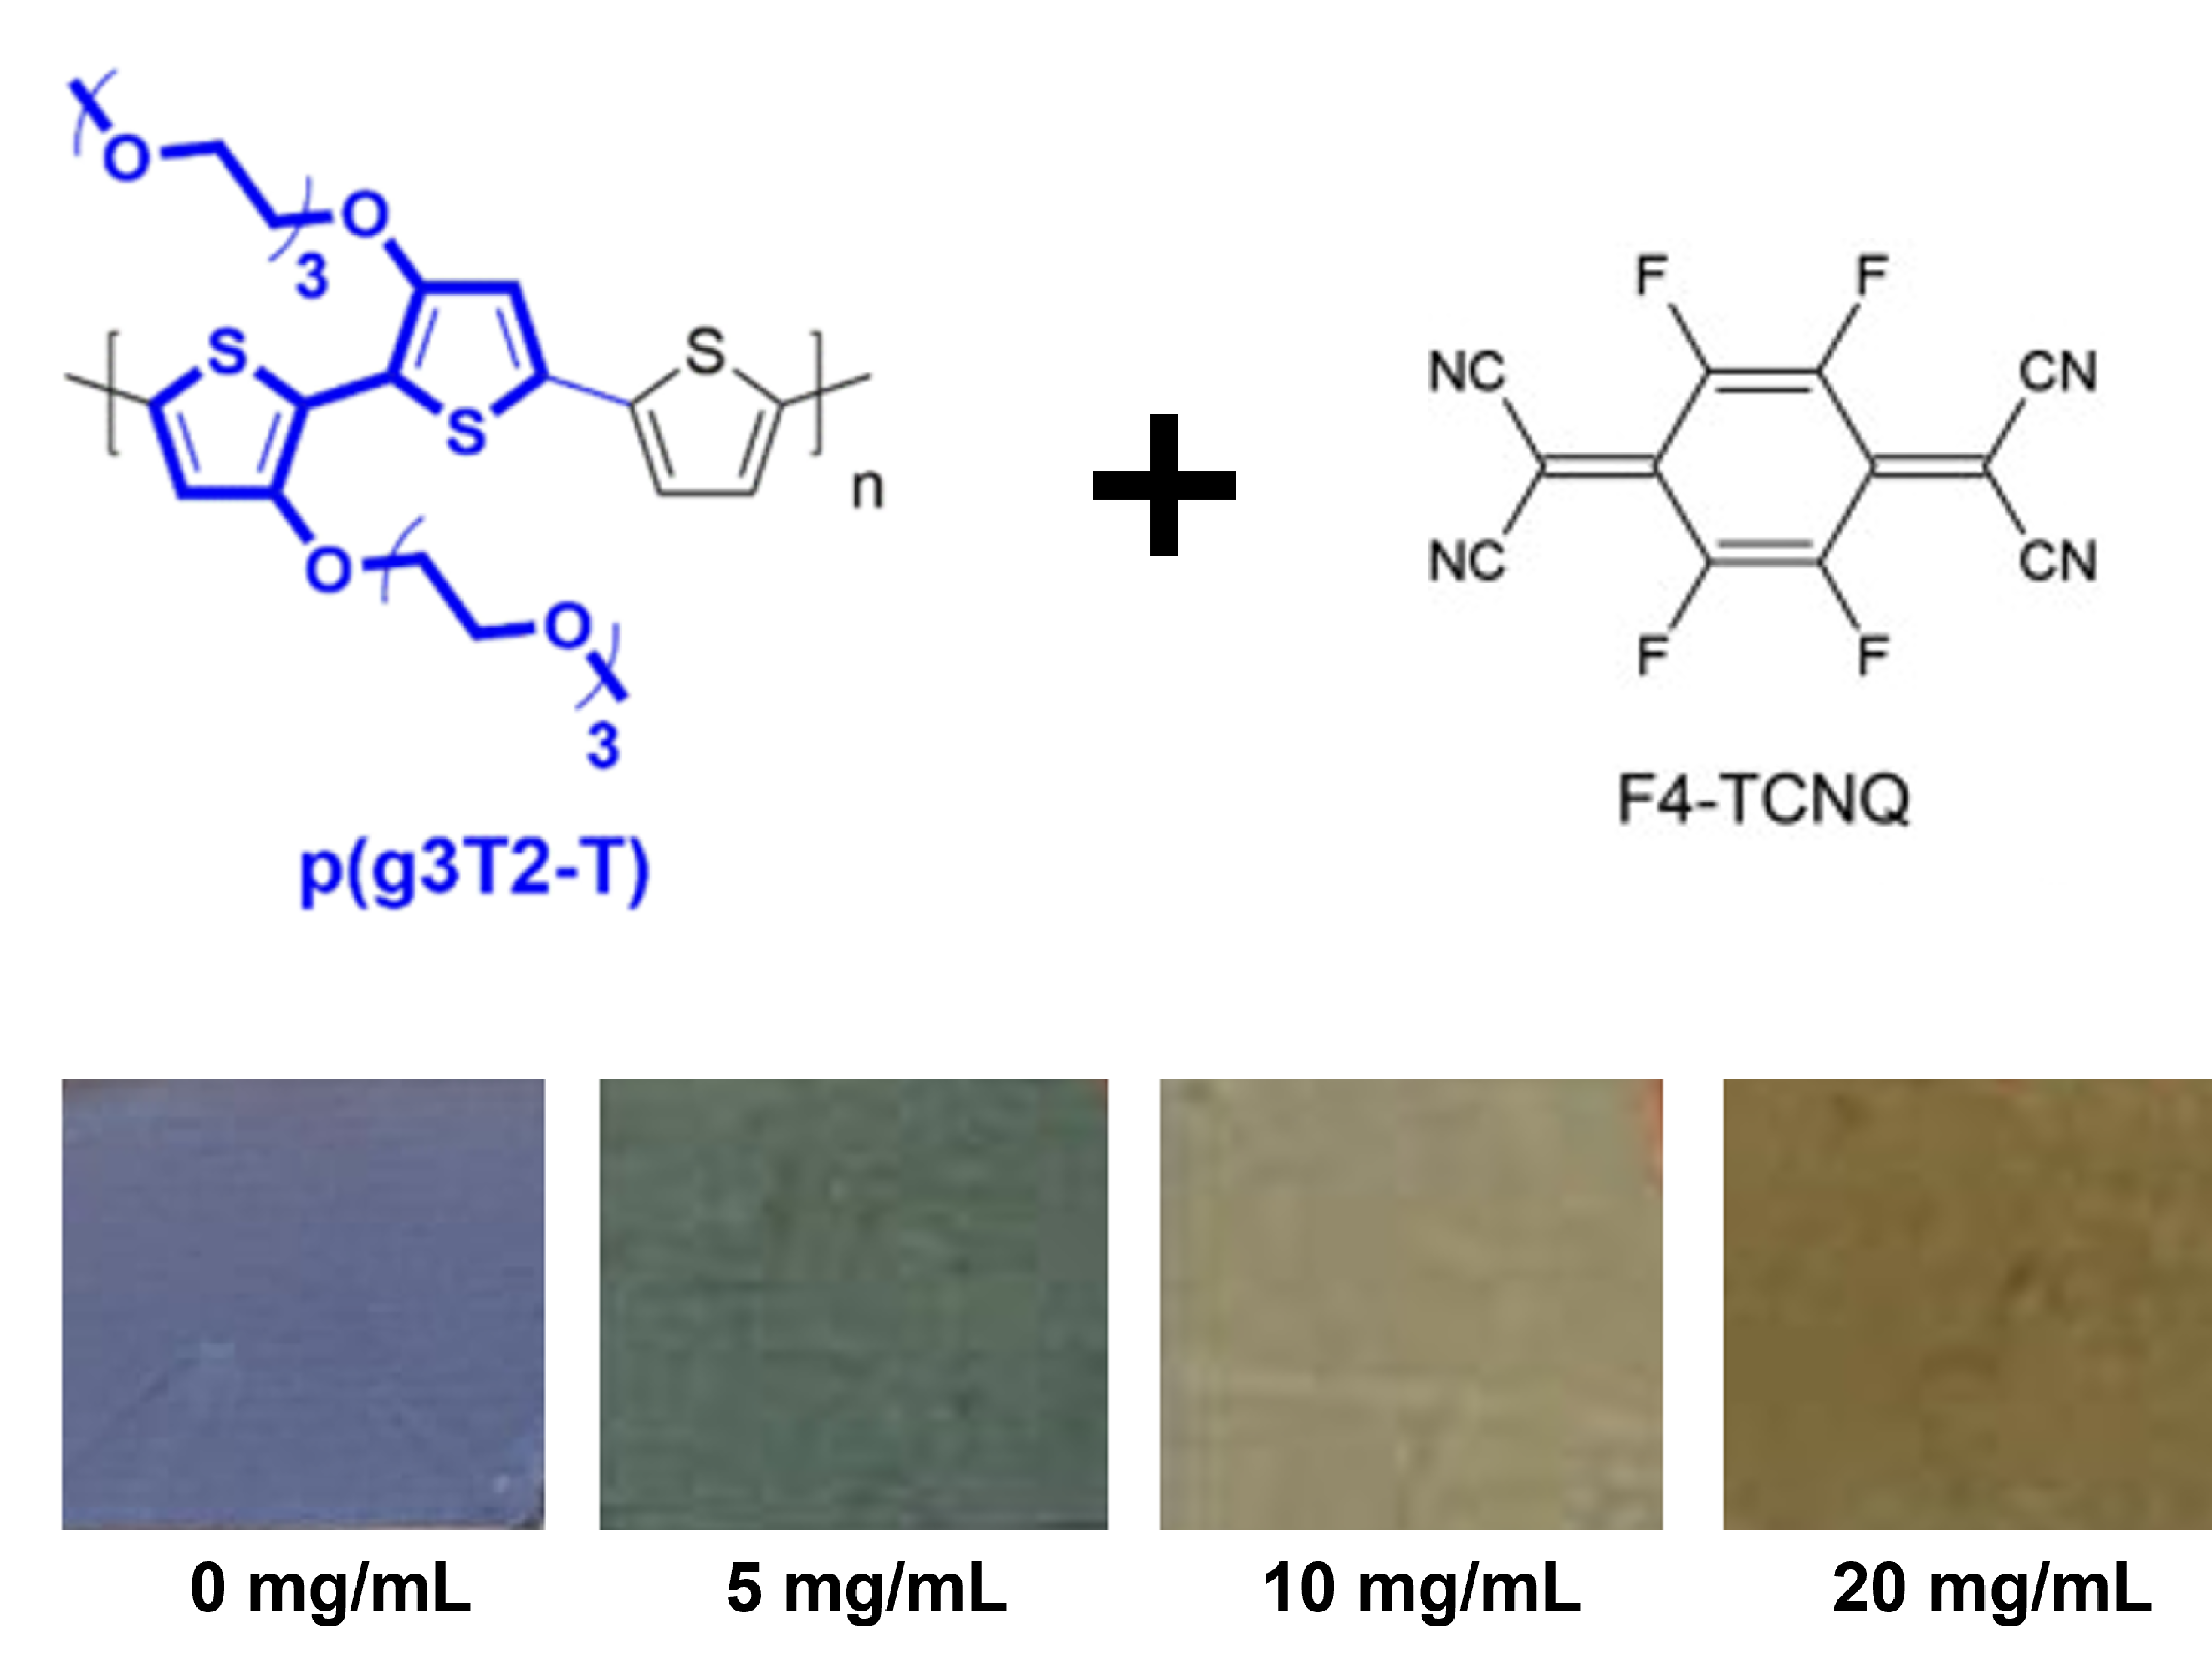
\includegraphics[width=9.5cm]{Images/pdf/doping_color.pdf}
  \caption[Color shift upon doping level increase]{Color change upon increasing dopant concentration from 0 to 20 mg/mL.
  \label{fig:color}}
\end{figure}

This color shift is expected as the optical properties of any material change upon doping. The spectra are discussed in more detailed later in this section.

\subsection{Thickness, Sheet Resistance, and Resistivity}

The film thickness was determined through profilometer measurements, resulting in an approximate thickness of 70 nm. Sheet resistance and resistivity were calculated using a four-point probe and the Van Der Pauw method, as shown in Table \ref{tab:res}. These calculations were performed using equations \ref{eq:rs} and \ref{eq:resist}, respectively, as described in the previous chapter. 

\begin{table}[ht]
\centering
\caption{Sheet resistance and resistivity values for undoped and doped films of p(g3T2-T) with F$_{4}$TCNQ.}
\begin{tabular}{l|c|c|c|c}
& Undoped & 5 mg/mL & 10 mg/mL & 20 mg/mL \\\hline
R$_{S}$ ($\Omega$/sq) & 6.3M & 104.6k & 70.7k & 49.4k\\
$\rho$ ($\Omega$cm) & 44.1 & 0.73 & 0.49 & 0.35\\\hline
\end{tabular}
\label{tab:res}
\end{table}

Upon doping, a substantial decrease is observed in both sheet resistance and resistivity. However, this decrease is not as pronounced when higher dopant levels are introduced, as depicted in Figure \ref{fig:rho}. %Nevertheless, when comparing the decrease among doped samples, a quasi-linear relationship becomes apparent with increasing the dopant concentration. 

\begin{figure}[ht]
  \centering
  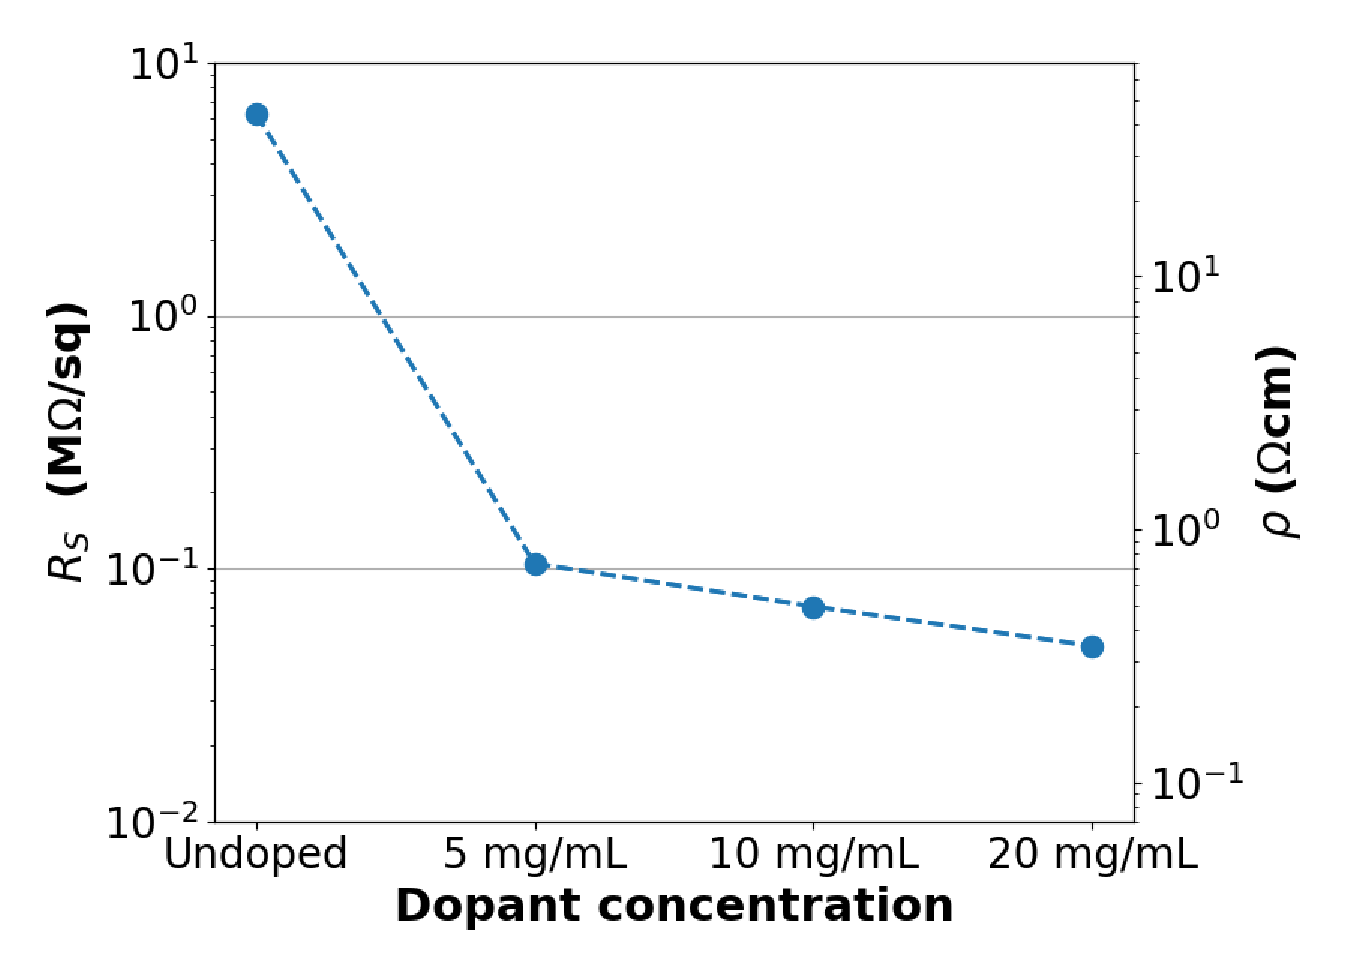
\includegraphics[width=8cm]{Images/pdf/resist.pdf}
  \caption[Sheet resistance and resistivity drop upon doping]{Sheet resistance and resistivity drop upon doping of p(g3T2-T) with F$_{4}$TCNQ. %Inset represents the quasi-linear drop of parameters as between doped samples.
  }
  \label{fig:rho}
\end{figure}

\subsection{Absorbance measurements}
The visible color hue shift can be quasi-quantitatively described by examining the absorbance spectra of the samples, as illustrated in Figure \ref{fig:abs}. In the case of undoped p(g3T2-T), there is a prominent absorption peak at 588 nm, which diminishes with increasing doping concentration, indicative of oxidation. Notably, new absorption peaks emerge at around 860 nm, a consequence of polaron generation, leading to new optical transitions, as explained in Section \ref{subsec:moldop}. 

\begin{figure}[ht]
  \centering
  %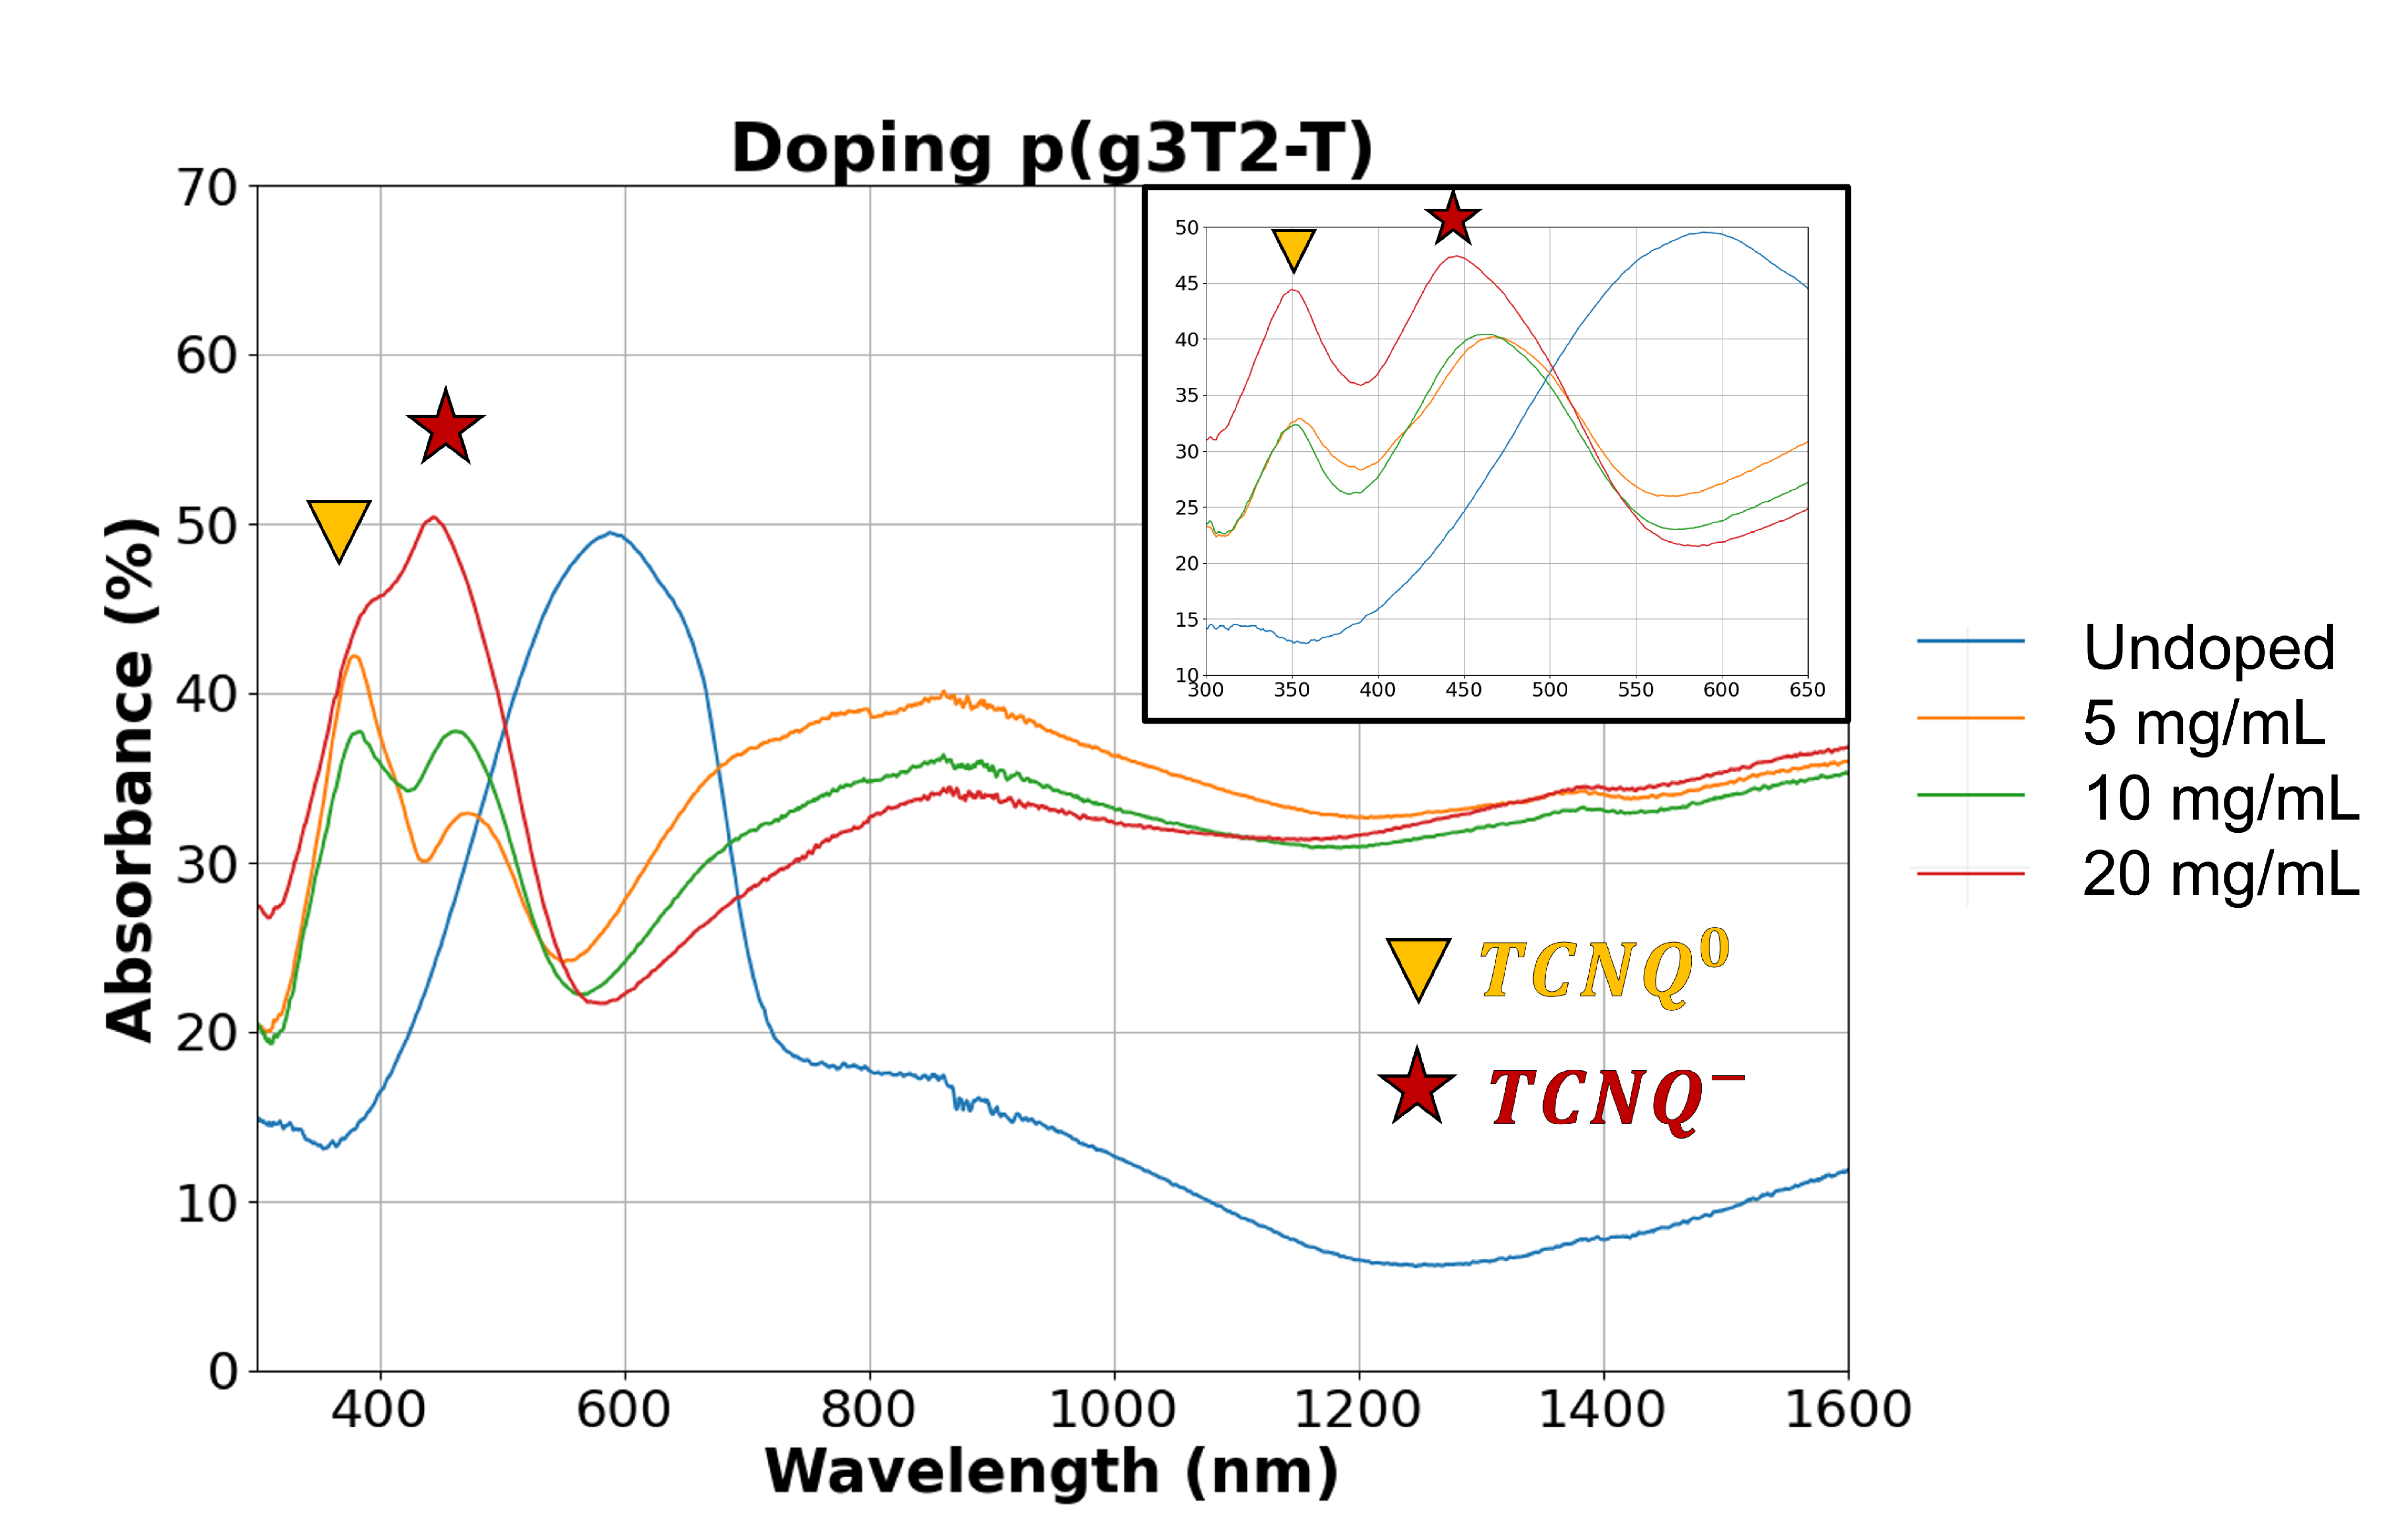
\includegraphics[width=11.5cm]{Images/pdf/abs+inlet.pdf}
  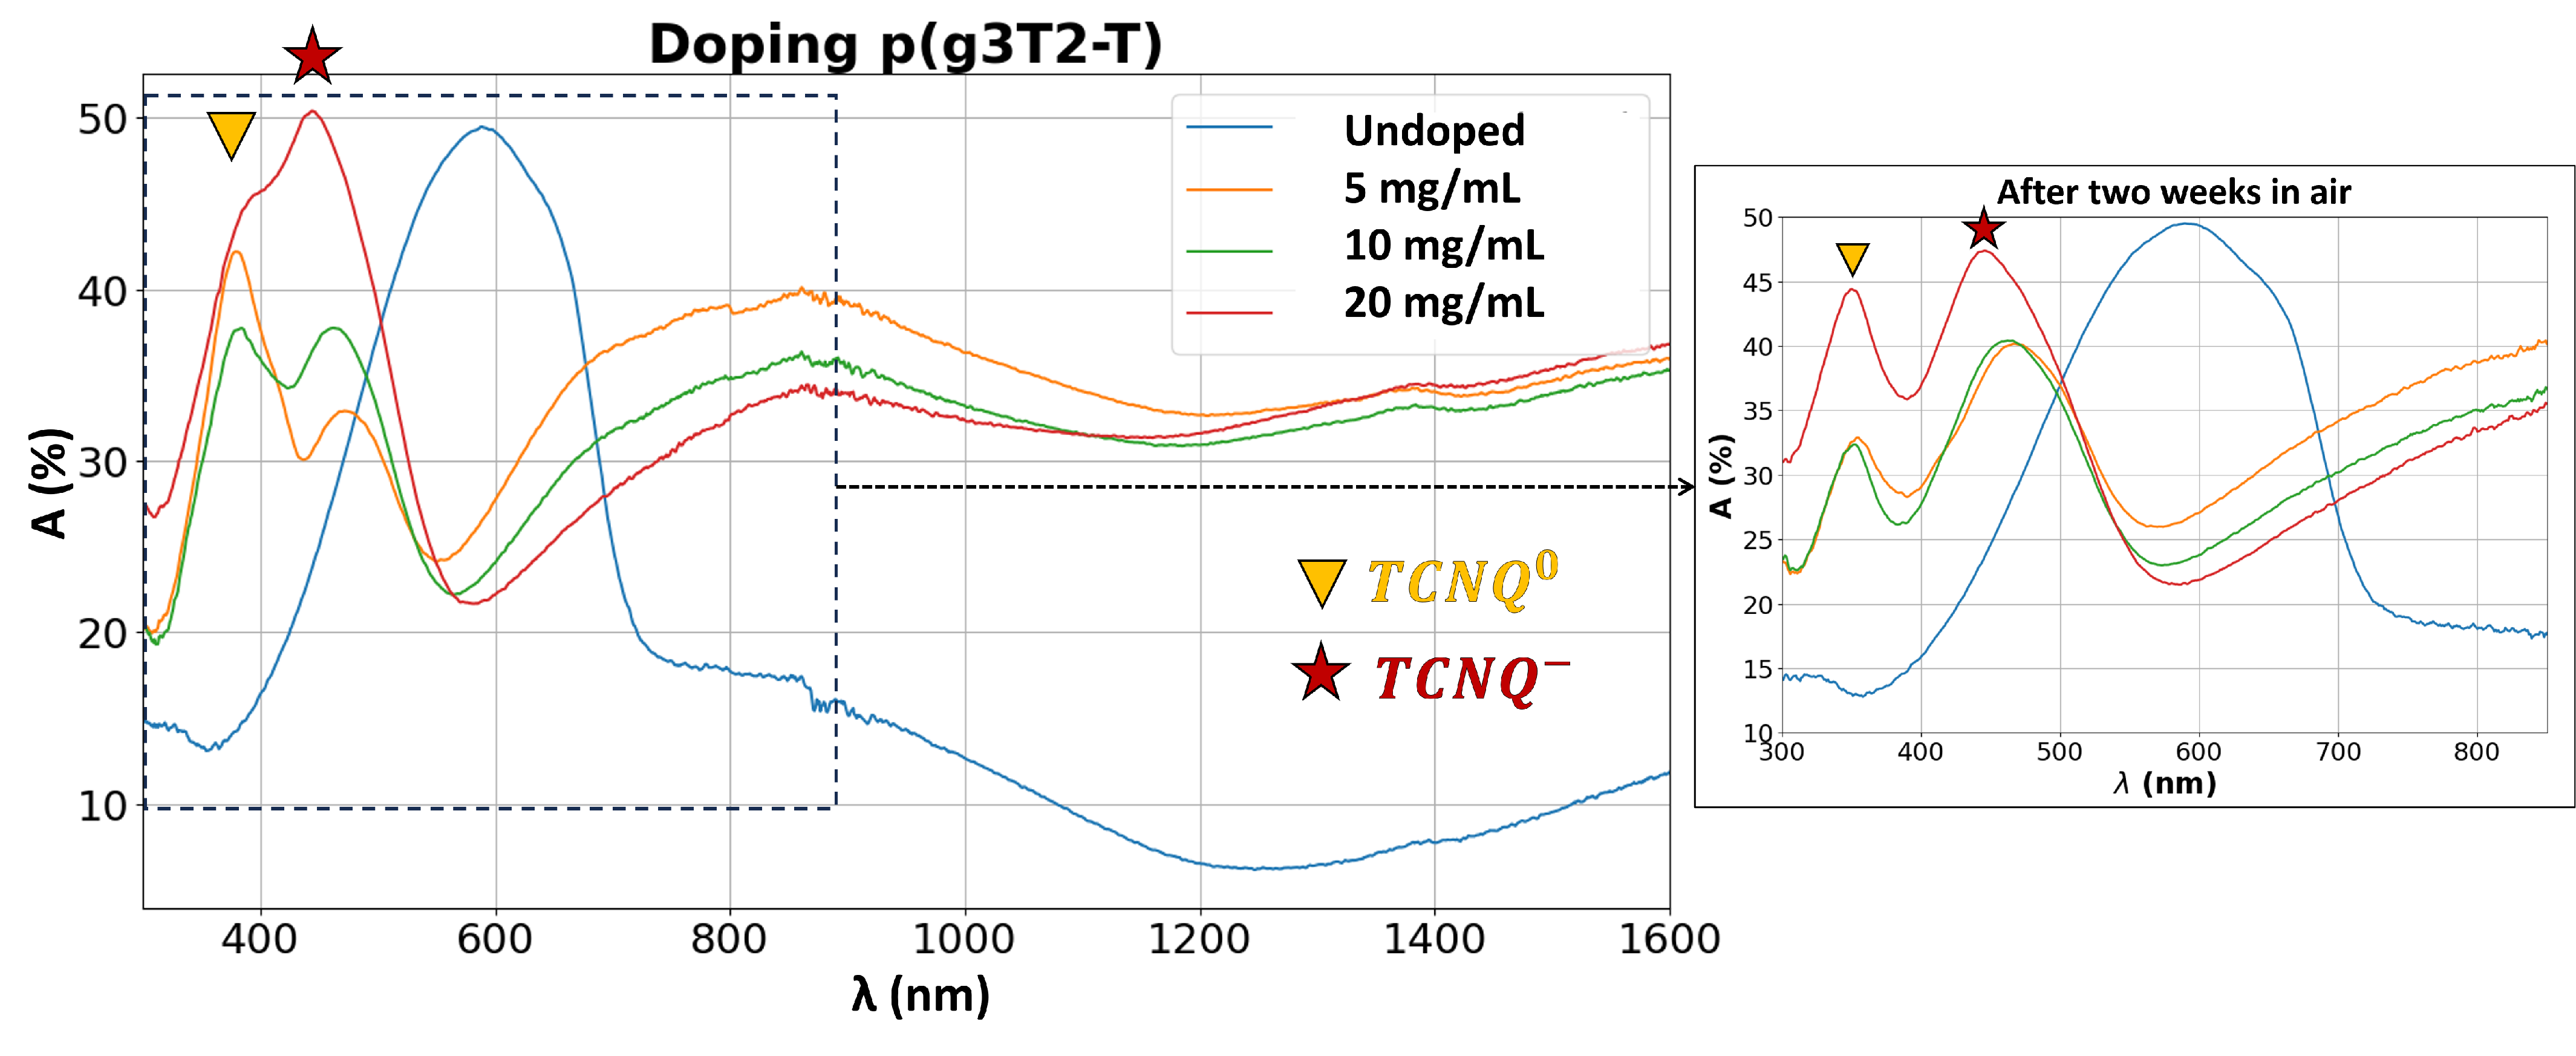
\includegraphics[width=\textwidth]{Images/pdf/abs_v2.pdf}  
  \caption[Absorbance spectra of different doping levels of p(g3T2-T)]{Spectra of undoped and doped p(g3T2-T) at different doping levels, corresponding to samples on Figure \ref{fig:color}. Figure at the right represents absorbance after two weeks of storage in ambient conditions.}
  \label{fig:abs}
\end{figure}

Tan et al. documented the appearance of new absorption peaks within the 300 to 600 nm range. The higher energy (lower wavelength) peak is generated by unreacted neutral dopant species (TCNQ$^{0}$), while the second is attributed to the new dopant anions (TCNQ$^{-}$), which induce charges in our polymer \cite{tanTuningOrganicElectrochemical2022}. Additionally, it is worth noting that, after several days of storage, the initially dominant peak of unreacted neutral dopants diminishes in intensity relative to the peak attributed to anions. This observation could be attributed to the ongoing diffusion of dopants through the polymer over time. Another contributing factor could be changes in the morphology. Further measurements are needed to confirm precise dopant concentration in polymer. 

Absorbance values are correlated with the density of states of these new optical transitions \cite{bredasPolaronsBipolaronsSolitons1985}. In our spectra, the absorbance value at 860 nm of the p(g3T2-T) sample with 5 mg/mL dopant concentration is relatively higher (around 40\%) compared to higher dopant levels. This finding might initially appear counterintuitive. However, as the doping concentration increases, the formation of bipolarons and bipolaron bands becomes energetically more favorable \cite{enenglDopinginducedAbsorptionBands2016}. This phenomenon aligns with observations in the higher wavelengths, such as at 1600 nm, where absorbance increases in the more highly doped p(g3T2-T) sample.

Moreover, Tan et al. reported the formation of bipolarons in this specific context, evidenced by a shift to lower energies in the broad absorbance spectrum within the mid-IR region (wavenumbers 1000-1600 cm$^{-1}$) \cite{tanTuningOrganicElectrochemical2022}. Consequently, further analysis of hole bipolaron formation can be conducted with Fourier Transform InfraRed (FTIR) spectroscopy.
 
\subsection{Workfunction}

In the context of studying electron energy levels in Ultraviolet Photoelectron Spectroscopy (UPS), the ideal film preparation involves working under inert conditions to prevent contamination. However, our current OECT fabrication process unavoidably exposes our films to ambient conditions. Consequently, we conducted measurements following deposition under these ambient conditions. As expected, UPS shows a shift of E$_{HBEC}$ and E$_{HOMO}$ values towards the Fermi level, which, in the material, is equivalent to an increase in the workfunction. This leads to a Fermi level shift towards the HOMO level as the dopant concentration increases, as depicted in Figure \ref{fig:ups}, which is characteristic of p-type doping. Unfortunately, potential contamination issues prevented the measurement of samples with a dopant concentration of 20 mg/mL, but the trend is clearly discernable.

\begin{table}[ht]
\centering
\caption{Calculated workfunction from UPS measurements and represented in Figure \ref{fig:ups}.}
\begin{tabular}{l|c|c|c}
& Undoped & 5 mg/mL & 10 mg/mL \\\hline
E$_{HBEC}$ [eV] & 17.35 & 16.47 & 16.36\\
E$_{HOMO}$ (vs E$_{F}$) & 4.28 & 3.27 & 3.24\\
WF [eV] & 3.87 & 4.28 & 4.86\\\hline
\end{tabular}
\label{tab:ups}
\end{table}

It is crucial to recognize that UPS is a surface-sensitive measurement. The penetration depth of the ultraviolet-range photons in UPS is limited to approximately 2 nm, significantly less than the thickness of our polymer film (approximately 70 nm). Consequently, this technique restricts our understanding of the diffusion of dopants throughout the entire volume of the polymer. Although, we gained some insights into this matter in the previous subsection, further analysis could be carried out using UPS with a depth-profiling option. 
%X-Ray Photoelectron Spectroscopy, which offers a depth profiling mode. %but along with depth profiling mode 3

\begin{figure}[ht]
	\centering
	\sidesubfloat[]{{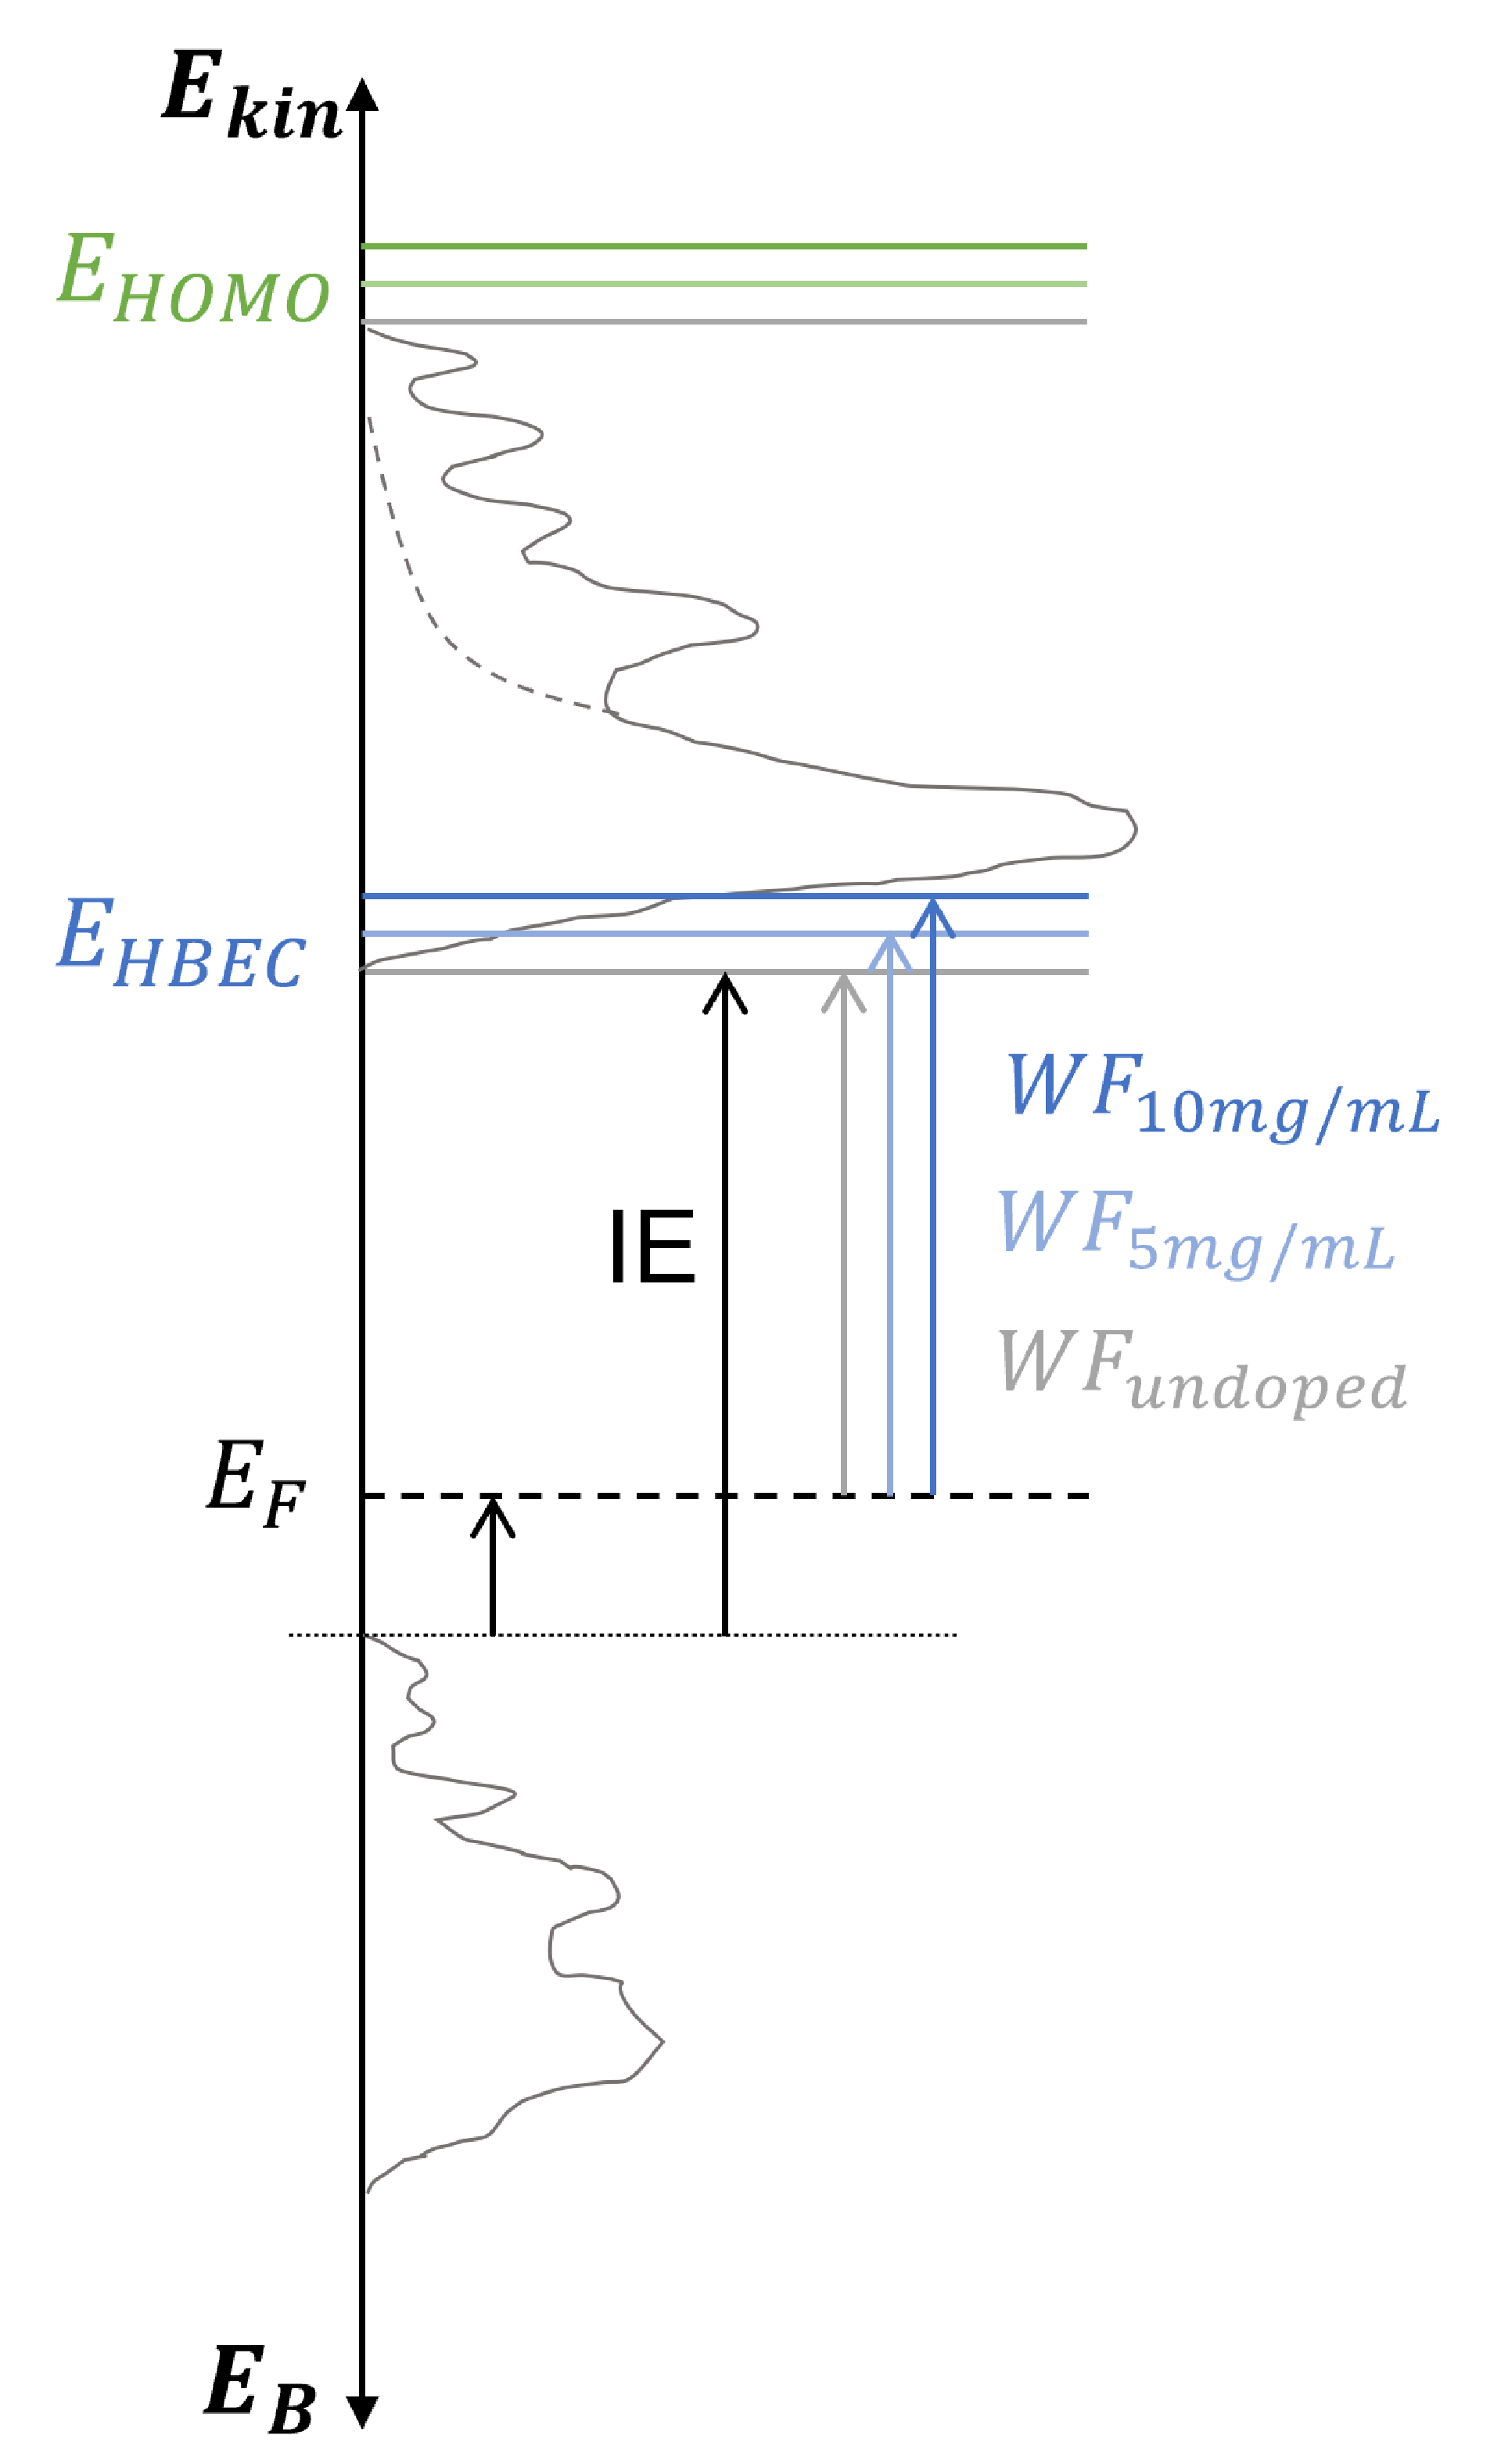
\includegraphics[width=6cm]{Images/pdf/WF_final.pdf} }}
	%\qquad
	%\hspace{2em}
	\sidesubfloat[]{{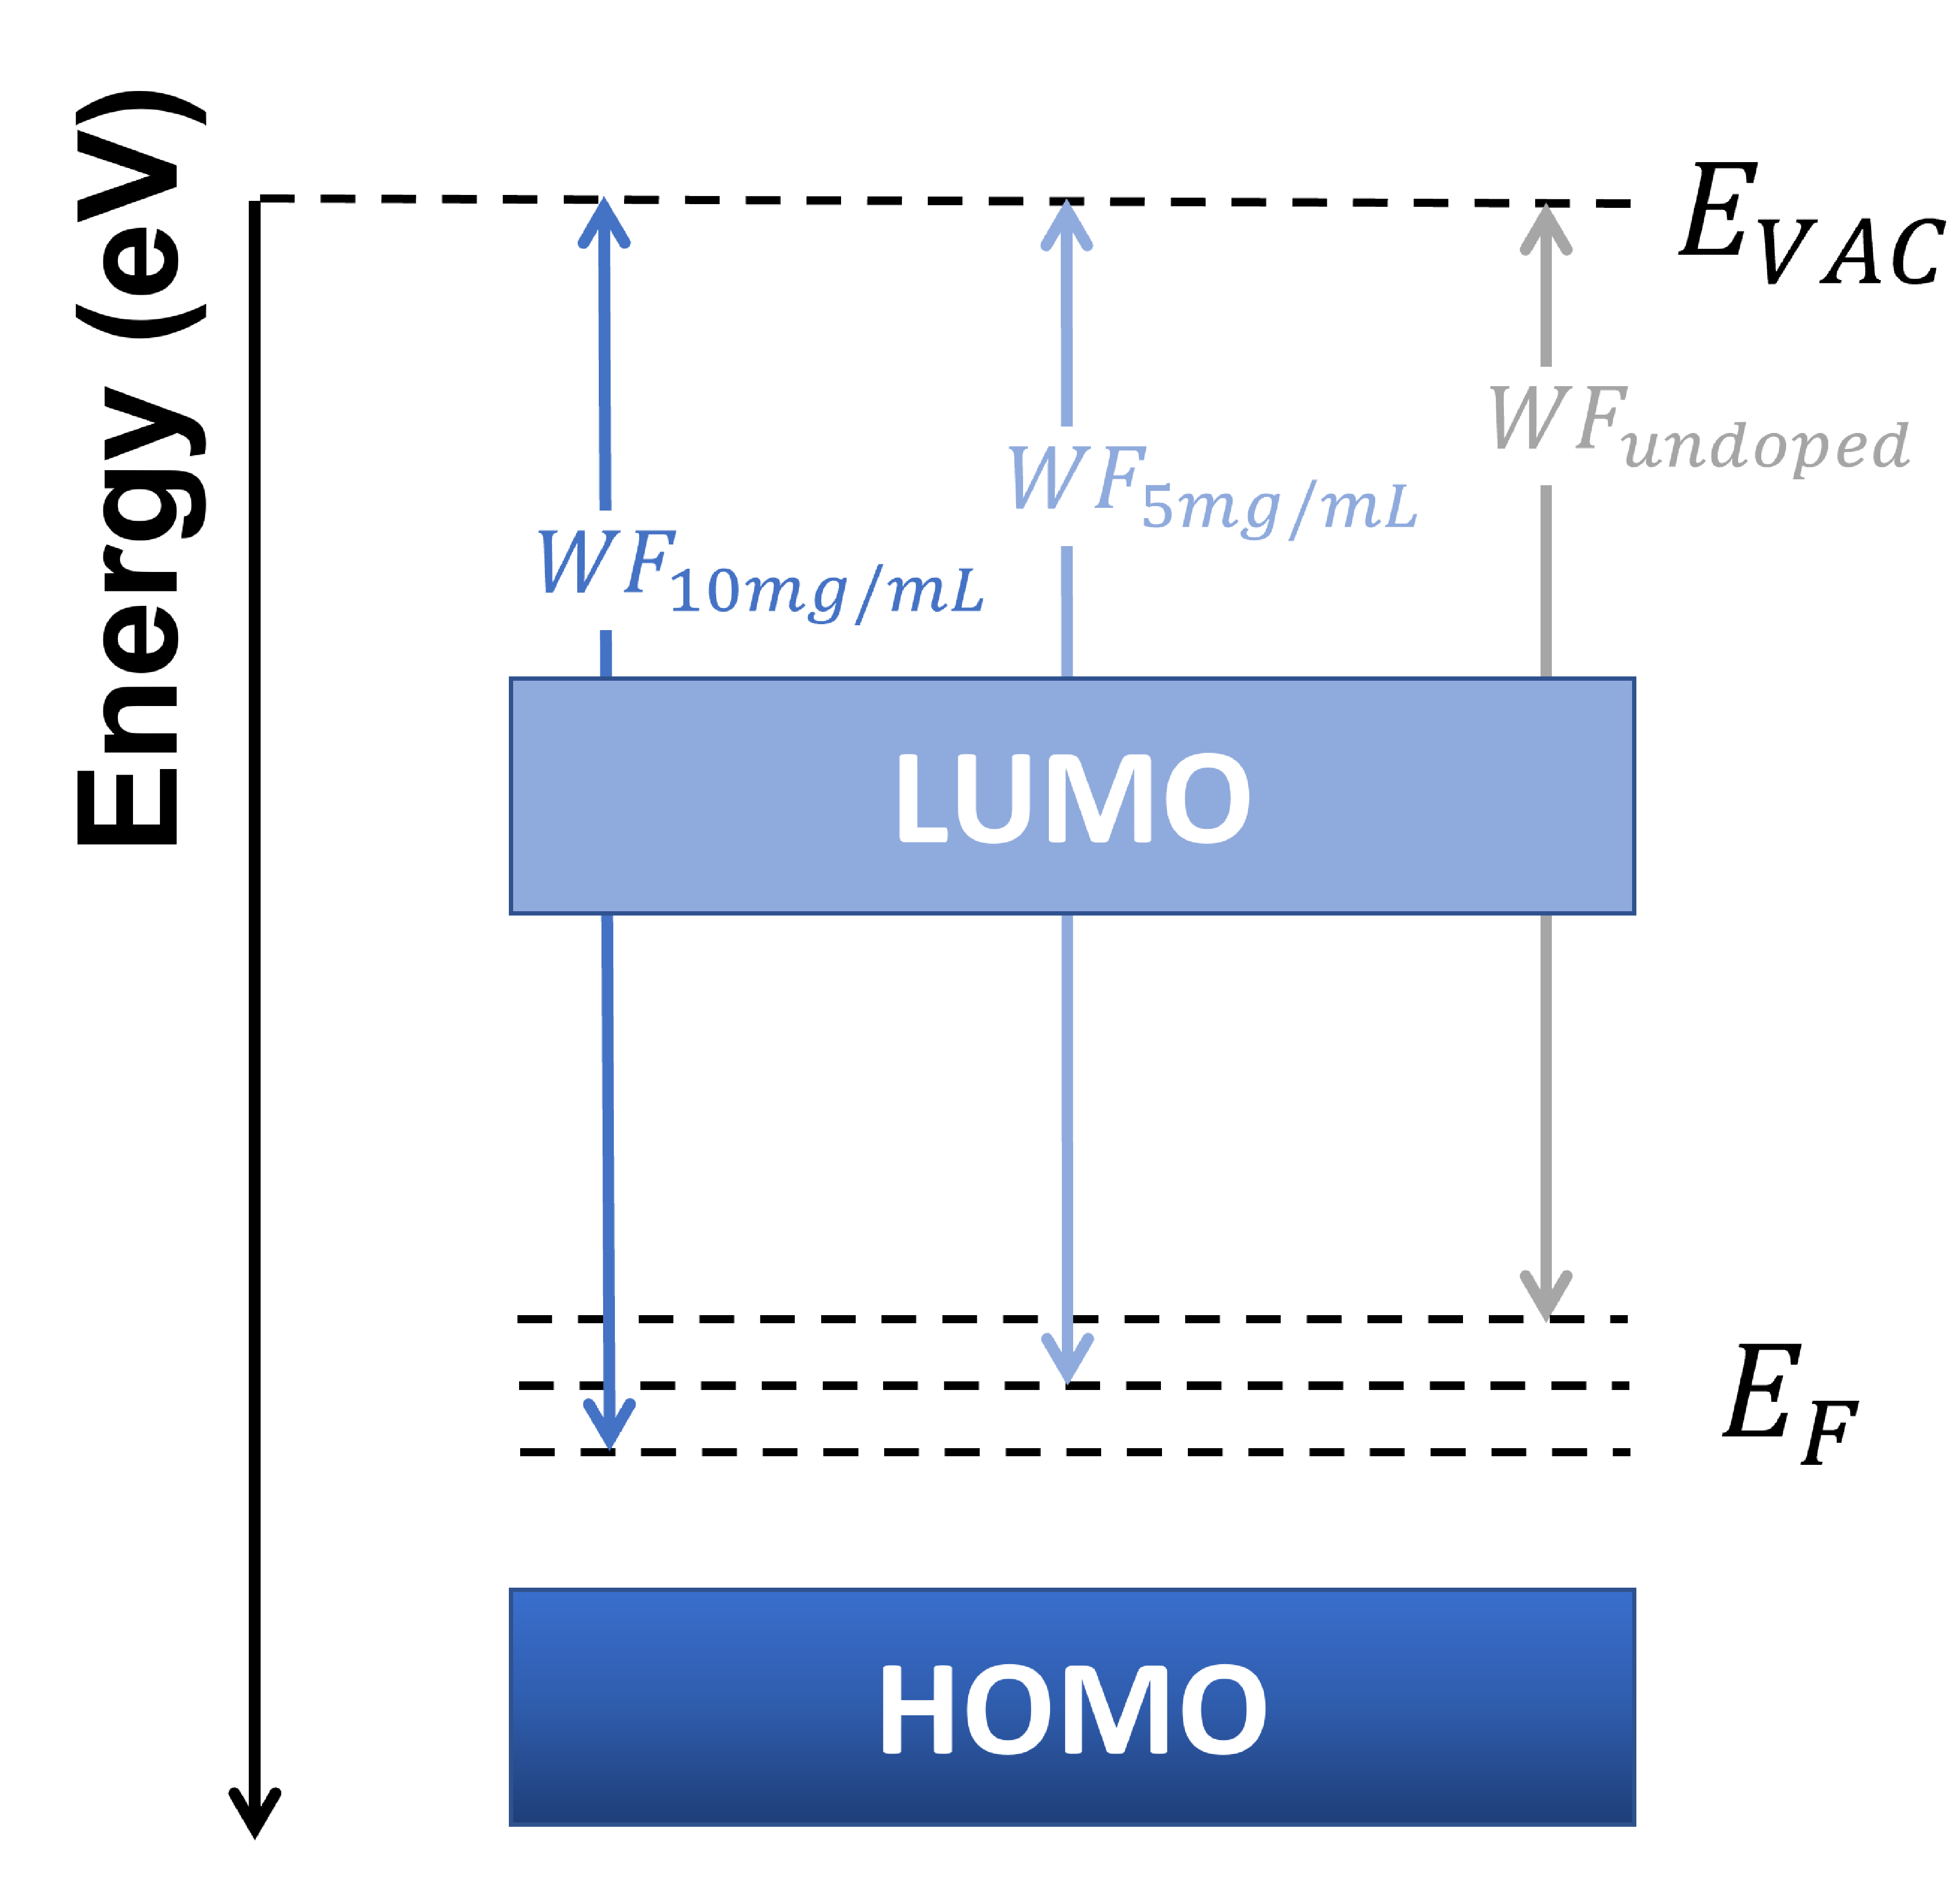
\includegraphics[width=6cm]{Images/pdf/WF.pdf} }}
	\caption[Representation of the Fermi level shift upon doping]{ Graphical representation of a) the relationship between the binding energies E$_{B}$ and the kinetic energy of the photoelectrons E$_{kin}$, and b) the Fermi level shift, upon doping.} 
	\label{fig:ups}
\end{figure}

%\subsection{Roughness}

%\section{Fabrication of Organic Electrochemical Transistors}
\section{Doping in Organic Electrochemical Transistors}
In the previous section, an investigation into doping levels with different F$_{4}$TCNQ concentrations was conducted. As expected, the samples exhibited an increase in conductivity, the formation of polarons and bipolarons, and an increase in the workfunction of the material as the dopant concentration increased. Now, our focus shifts to the fabrication of OECTs.

Our ultimate goal is to study fully patterned solid-state OECTs that will enable integrated circuits (IC) and thermodynamic studies \cite{cucchiThermodynamicsOrganicElectrochemical2022}. Consequently, it was imperative to initially investigate the isolated impact of channel doping on our devices. Therefore, as detailed in the previous chapter, we will pair our channel with a non-polarizable gate, such as a Ag/AgCl, a widely used configuration for investigating OECT-based materials. This will be coupled with a Solid-State Electrolyte (SSE) precursor, the specific composition was outlined in Table \ref{tab:sse} of Chapter \ref{cha:2}.

We have formulated two hypotheses, based on reference \cite{tanTuningOrganicElectrochemical2022}, regarding the expected performance of our devices:

\begin{enumerate}
\item Transfer characteristics may be adversely impacted by channel doping.

\item The introduction of ionic species (TCNQ$^{-}$) into p(g3T2-T) films should result in depletion-mode devices with positive threshold voltages. This is because a higher positive gate bias would be needed to counteract these anions and turn off the device.
\end{enumerate}

%Prior biasing gate, which is due to passive (ion) diffusion?

\subsection{Influence of Doping on OECT Channel}
The patterning process was successfully accomplished via photolithography, as detailed in Section \ref{subsec:channel}, employing a mask that included a microstructured gate. This setup is ideal for studying OECTs with both channel and gate constructed from the same OMIEC material, commonly PEDOT:PSS. The result of this process is displayed in Figure \ref{fig:channel}. 

\begin{figure}[ht]
  \centering
  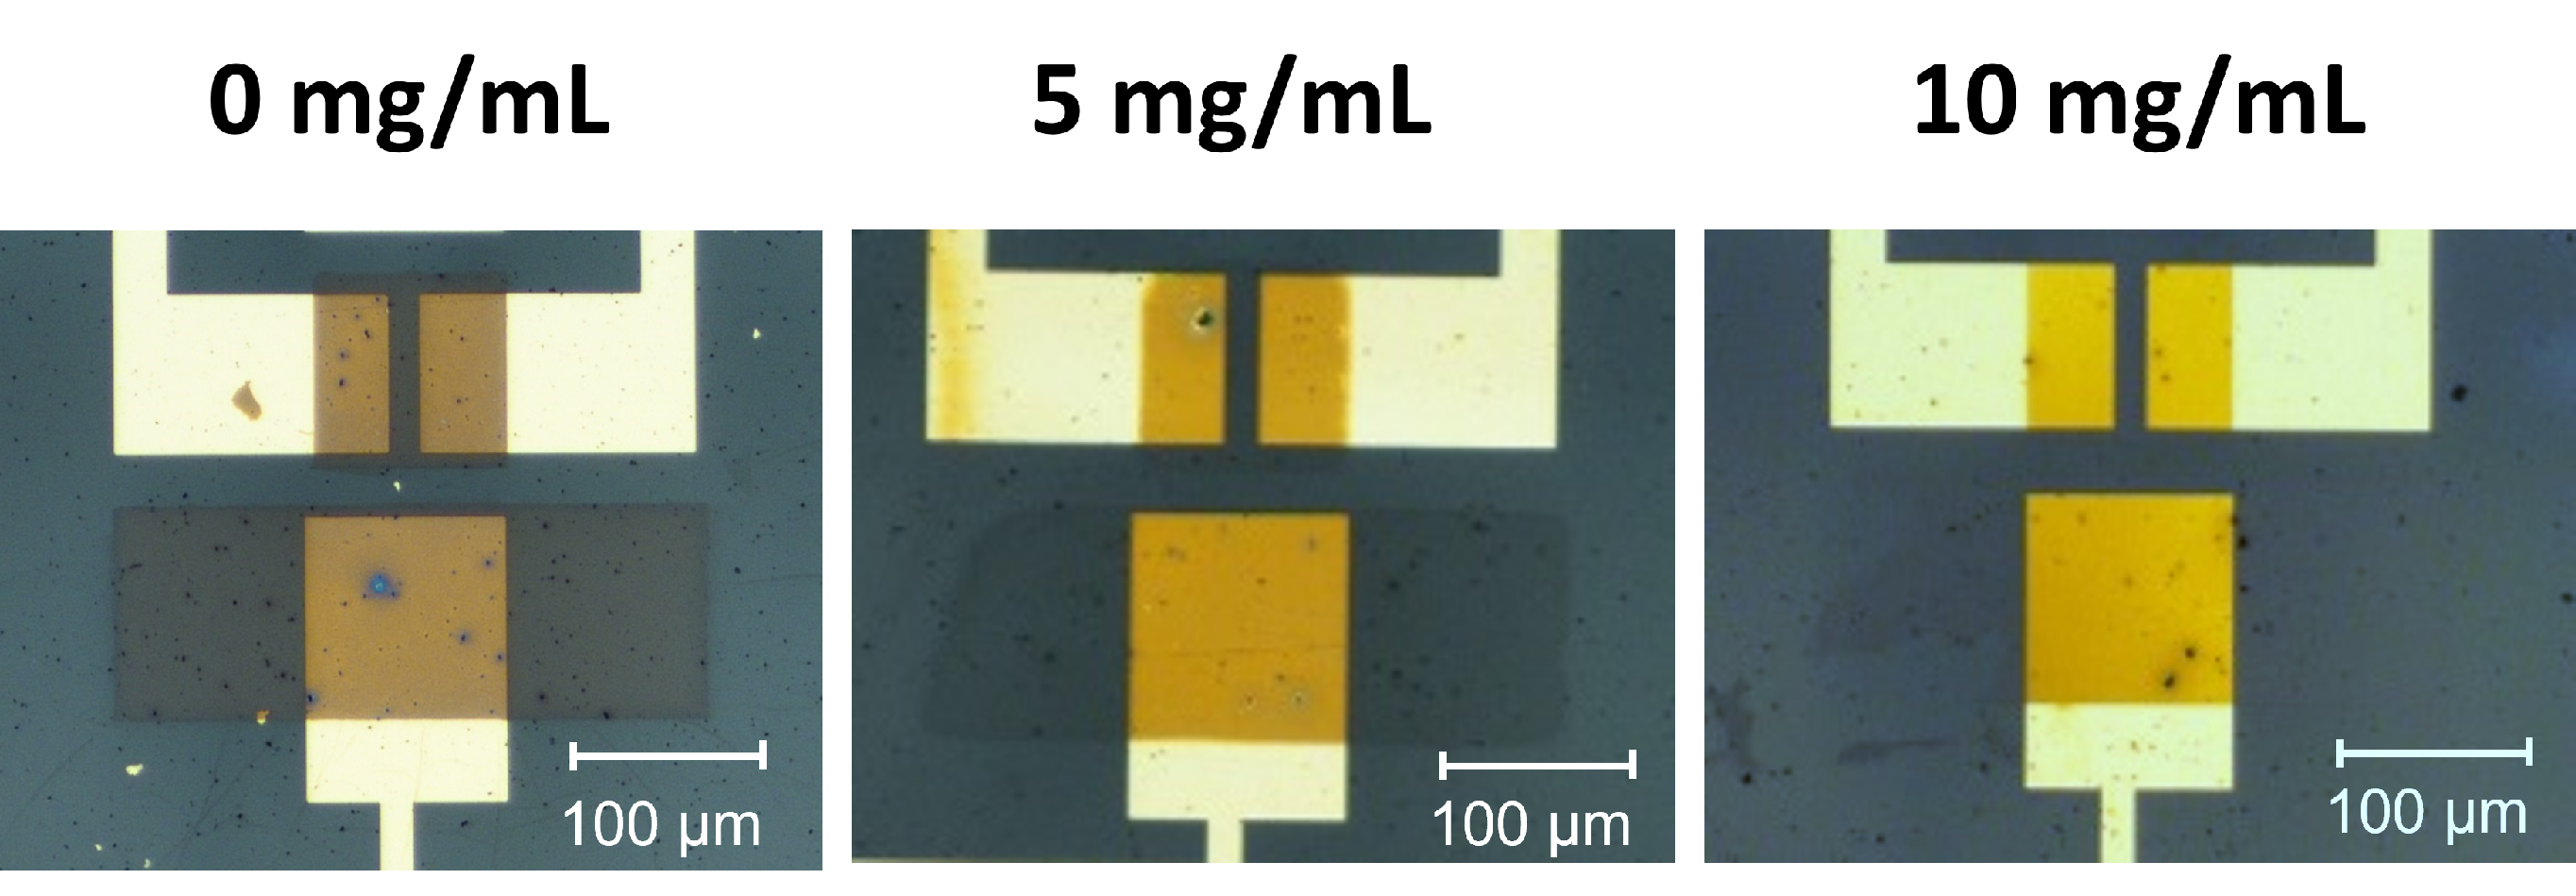
\includegraphics[width=11cm]{Images/pdf/BigGateDevices.pdf}
  \caption[Micrographs of a patterned channel and gate p(g3T2-T) at different doping levels]{Micrographs of patterned channel and gate with p(g3T2-T) undoped, 5 mg/mL and 10 mg/mL dopants, following procedures explained in Section \ref{subsec:channel}.}
  \label{fig:channel}
\end{figure}

%Our ultimate goal is to study fully patterned solid-state OECTs that will enable integrated circuits (IC) and thermodynamic studies \cite{cucchiThermodynamicsOrganicElectrochemical2022}. To achieve this, it was imperative to initially investigate the isolated impact of channel doping on our devices. Several hypothesis were formulated, based on reference \cite{tanTuningOrganicElectrochemical2022}:

%\begin{enumerate}
%\item Modifying channel doping may adversely impact transfer characteristics.
%\item The introduction of ionic species (TCNQ$^{-}$) into p(g3T2-T) films should result in depletion-mode devices with positive threshold voltages. This is because a higher positive gate bias would be needed to counteract these anions and turn off the device.
%\end{enumerate}

%As explained in the previous chapter, we paired our channel with a non-polarizable gate such as a Ag/AgCl, a widely used configuration for investigating OECT-based materials, and coupled it with a Solid-State Electrolyte (SSE) precursor, whose specific composition was outlined in Table \ref{tab:sse} of Chapter \ref{cha:2}. Unfortunately, sample that used a solution with a dopant concentration of 20 mg/mL exhibited issues with doping homogeneity due to a possible contamination of the mixture. While photolithography was still feasible, it could not provide a fair basis for comparison with the other devices. Consequently, this sample will be excluded from our analysis.

The results shown in Figures \ref{fig:transx2} - \ref{fig:vth_vds} correspond to the same device and the same loop on each sample (undoped, 5 mg/mL, and 10 mg/mL dopants) from the same batch of materials. After reporting the analysis of individual devices, a more comprehensive statistical study will be conducted on operational devices from each sample. 

It is essential to note that for the statistical analysis of this section, despite our efforts to increase the yields, only 3 or 4 out of the 14 devices were operational in each sample. The undoped polymer exhibited a strong affinity with the photoresist, complicating the development process. Additionally, samples with higher dopant concentrations required longer UV light exposure times, and overdevelopment ocurred more frequently, resulting in lower yields. Optimization for specific parts of the process were necessary and ultimately accomplished, and will be detailed in subsequent sections of this chapter. 
%% Details on low yields in reviewed of KL

Transfer characteristics are illustrated in Figure \ref{fig:transx2}a, c, e, corresponding to undoped, 5 mg/mL, and 10 mg/mL dopants, respectively. Notably, a positive turn-on voltage is observed in the undoped OECT device, indicating the rapid oxidation (unwanted) of p(g3T2-T) under environmental conditions due to its low ionization potential (IP). 

The drain current ($I_{D}$) of the undoped device exhibits higher values than doped devices. Hidalgo Castillo et al.  \cite{hidalgocastilloSimultaneousPerformanceStability2022a} reported that pristine p(g3T2-T) exhibits a oxygen reduction reaction (ORR) activity in oxygen-saturated conditions, resulting in an increase in current within the polymer until saturation. To address this issue, it will be necessary to control the oxidation state of the polymer during selective steps of the fabrication process or find a way to reverse the oxidation of p(g3T2-T), which will be explored in subsequent sections.

\begin{figure}[!ht]
    \centering
    %\subfloat[Undoped device]{{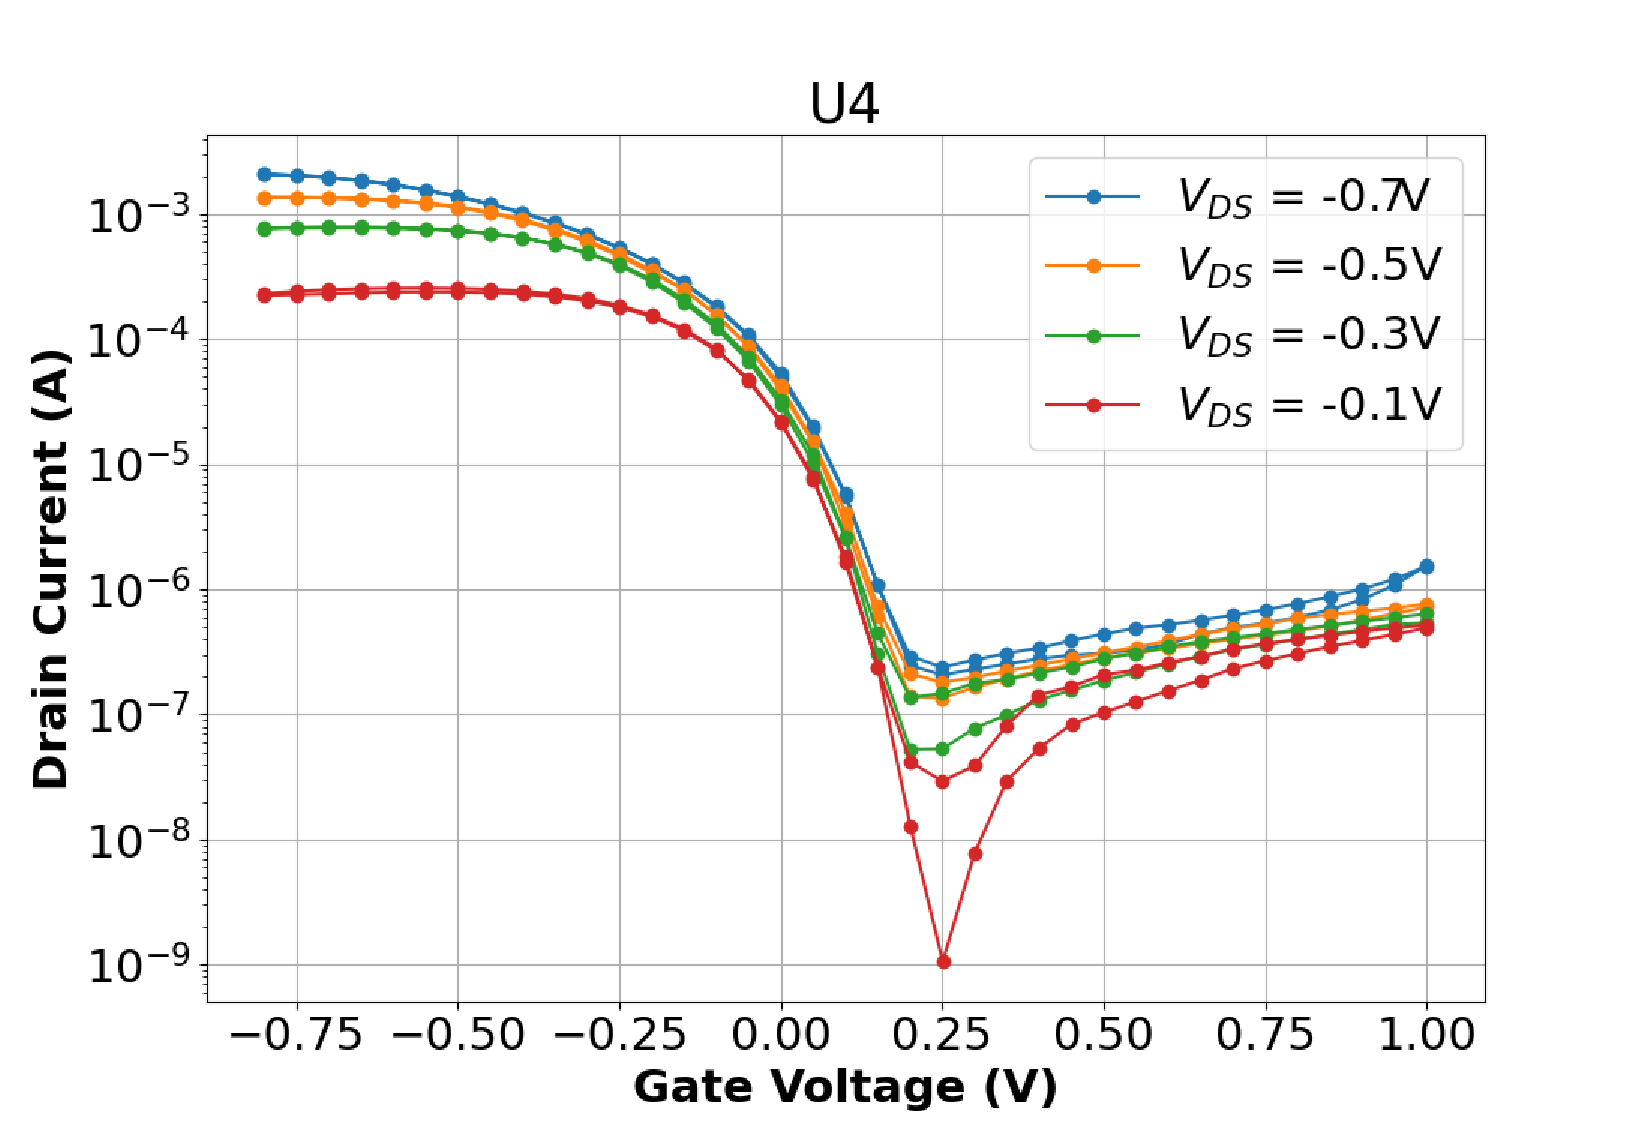
\includegraphics[width=7.1cm]{Images/pdf/transfer_undoped.pdf} }}
    %\subfloat[Undoped device]{{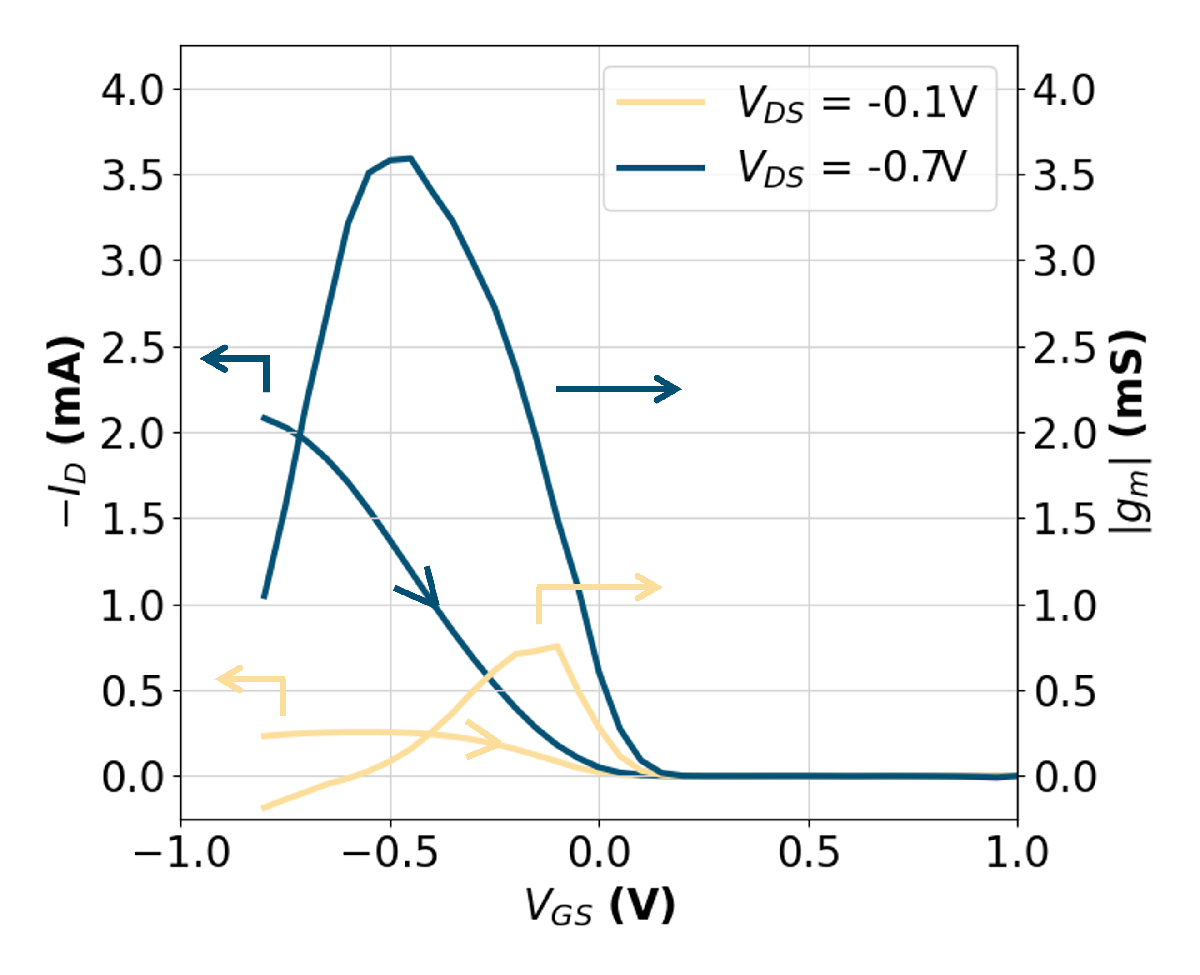
\includegraphics[width=6.7cm]{Images/pdf/id+gm_undoped_final.pdf} }}
    %\qquad
    %\subfloat[5 mg/mL dopant device]{{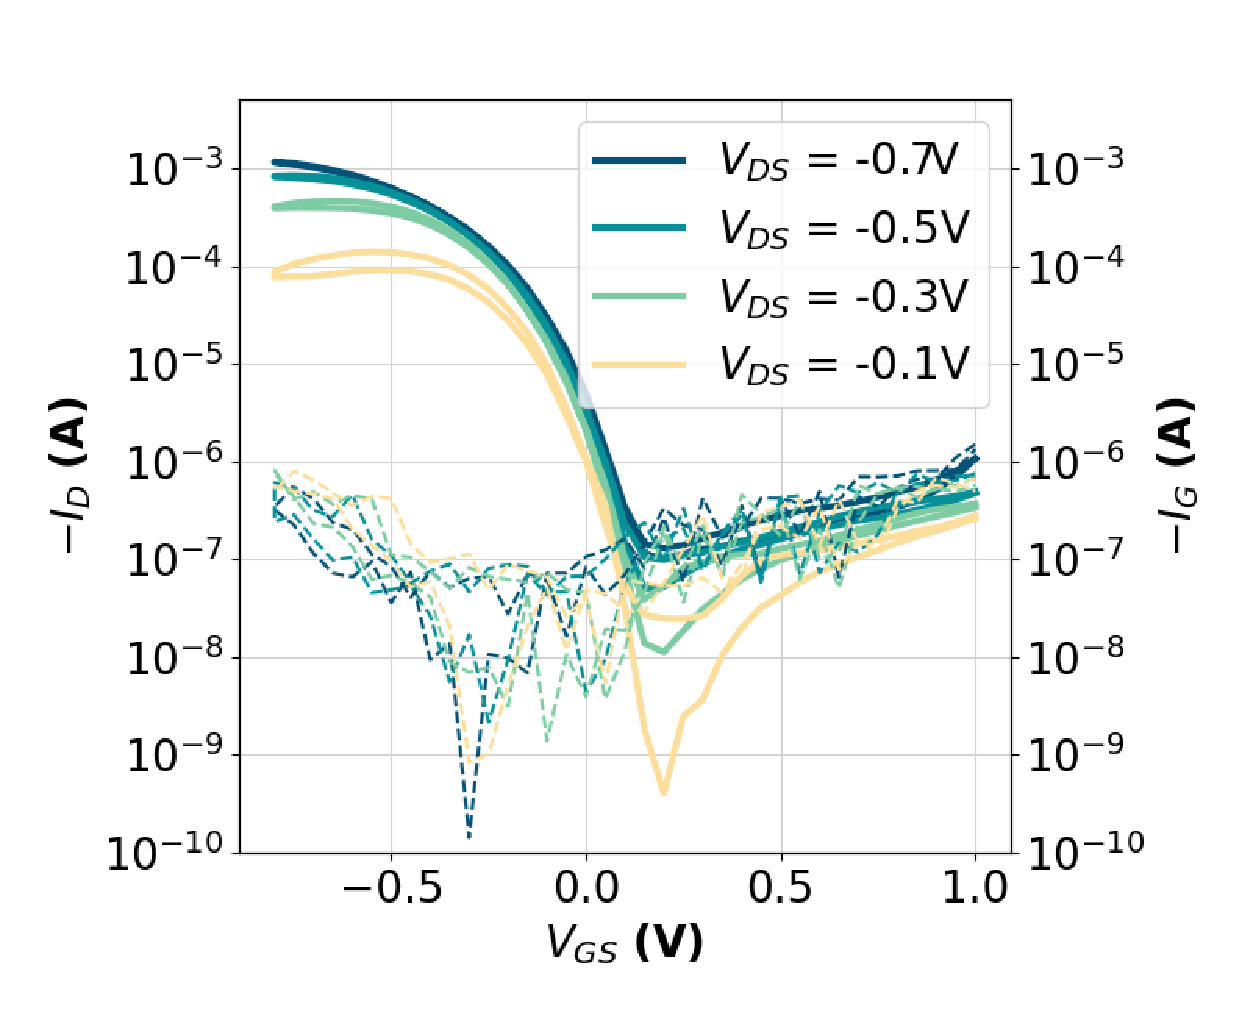
\includegraphics[width=7.1cm]{Images/pdf/transfer_doped5.pdf} }}
    %\subfloat[5 mg/mL dopant device]{{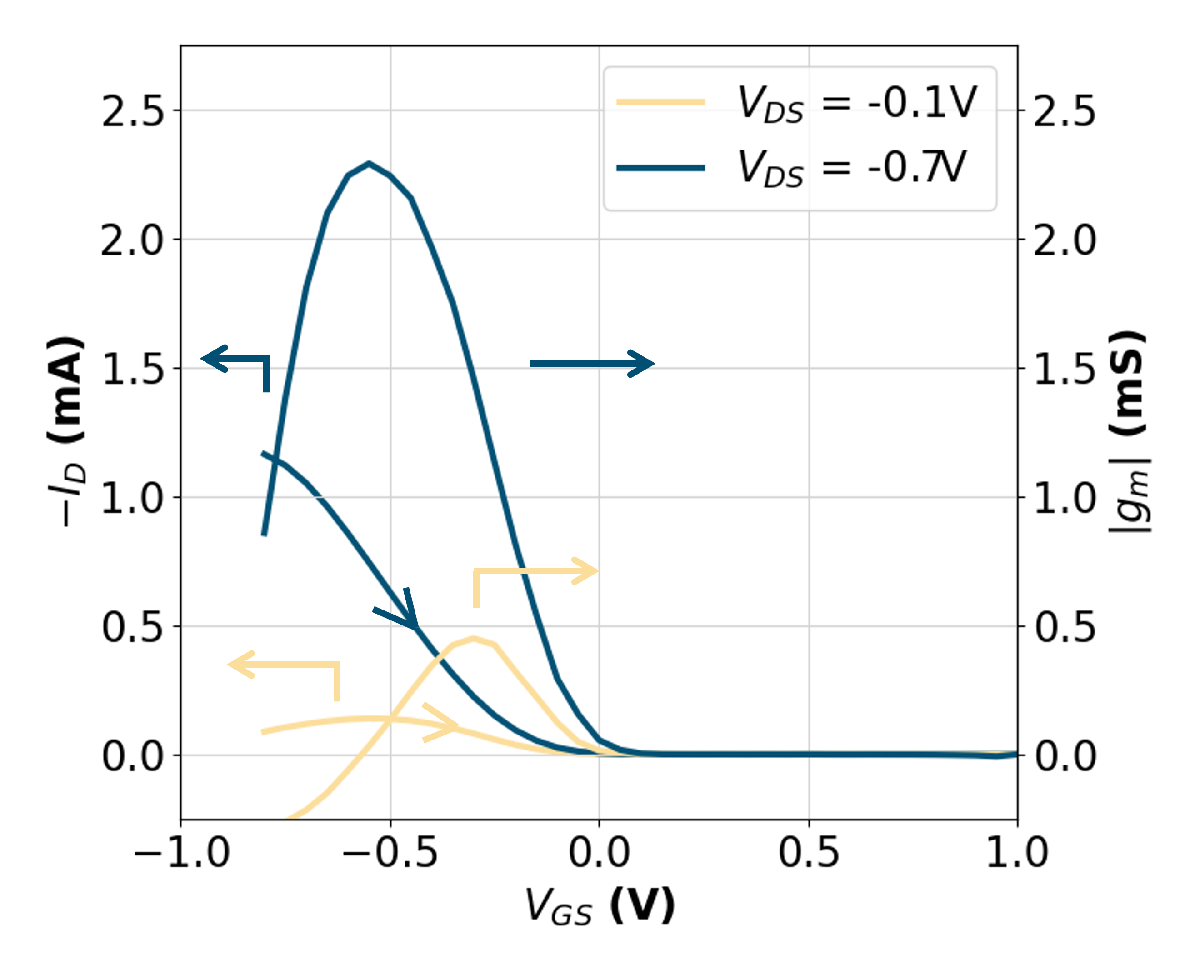
\includegraphics[width=6.7cm]{Images/pdf/id+gm_doped5_final.pdf} }}
    \includegraphics[width=\textwidth]{Images/pdf/transx2.pdf} 
\caption[Transfer characteristics and transconductance at different doping levels and $V_{DS}$]{a), c) , e) Transfer characteristics of all measured $V_{DS}$ including the gate leakage current $I_{G}$ b), d), f) Transfer curves (off-switching) with corresponding transconductance. Each group of graphs for undoped and 5 mg/mL and 10 mg/mL doped p(g3T2-T) channel, respectively.}
    \label{fig:transx2}
\end{figure}
    
%U4 loop 2 as undoped pattern
%U2 loop 3 for doped 5
%U4 loop 3 for doped 10

Gate current ($I_{G}$) is represented by dotted lines, and it is apparent that the drain OFF current ($I_{D,OFF}$) is dominated by this leakage current in all devices. %Figure \ref{fig:shift1} shows that doped devices exhibit minimal differences in $I_{D,OFF}$.

\begin{table}[ht]
\centering
\caption{Maximum transconductance values extracted from Figure \ref{fig:transx2}}
\begin{tabular}{l|c|c|c}
|g$_{m,max}$| [mS] @ & Undoped & 5 mg/mL & 10 mg/mL \\\hline
$V_{DS}$ = -0.1 V & 0.75 & 0.45 & 0.24\\
$V_{DS}$ = -0.3 V & 2.01 & 1.31 & 0.74\\
$V_{DS}$ = -0.5 V & 2.90 & 1.97 & 1.09\\
$V_{DS}$ = -0.7 V & 3.59 & 2.23 & \\ \hline
\end{tabular}
\label{tab:trans}
\end{table}

Notably, the device with the highest dopant concentration (10 mg/mL dopant) shows signs of breakage as $V_{DS}$ becomes more negative (Figure \ref{fig:transx2}e and Figure \ref{fig:shift1}d). Consequently, this measurement will be excluded from the calculation of transconductance and threshold voltage.

\begin{figure}[ht]
    \centering
    %\sidesubfloat[]{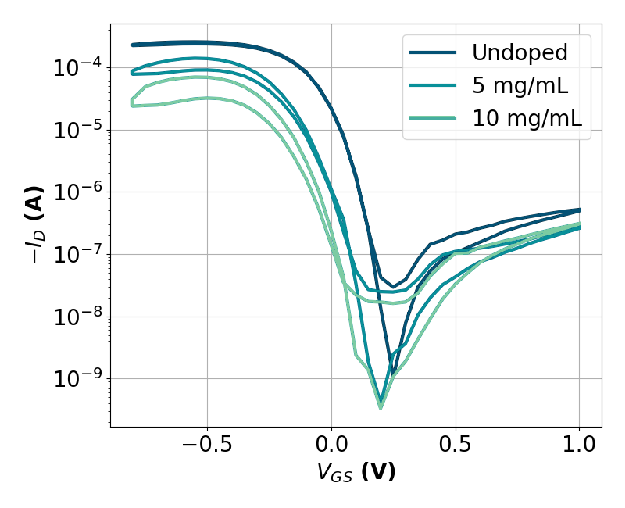
\includegraphics[width=7cm]{Images/pdf/Shift_Vds1.pdf} }
    %\sidesubfloat[]{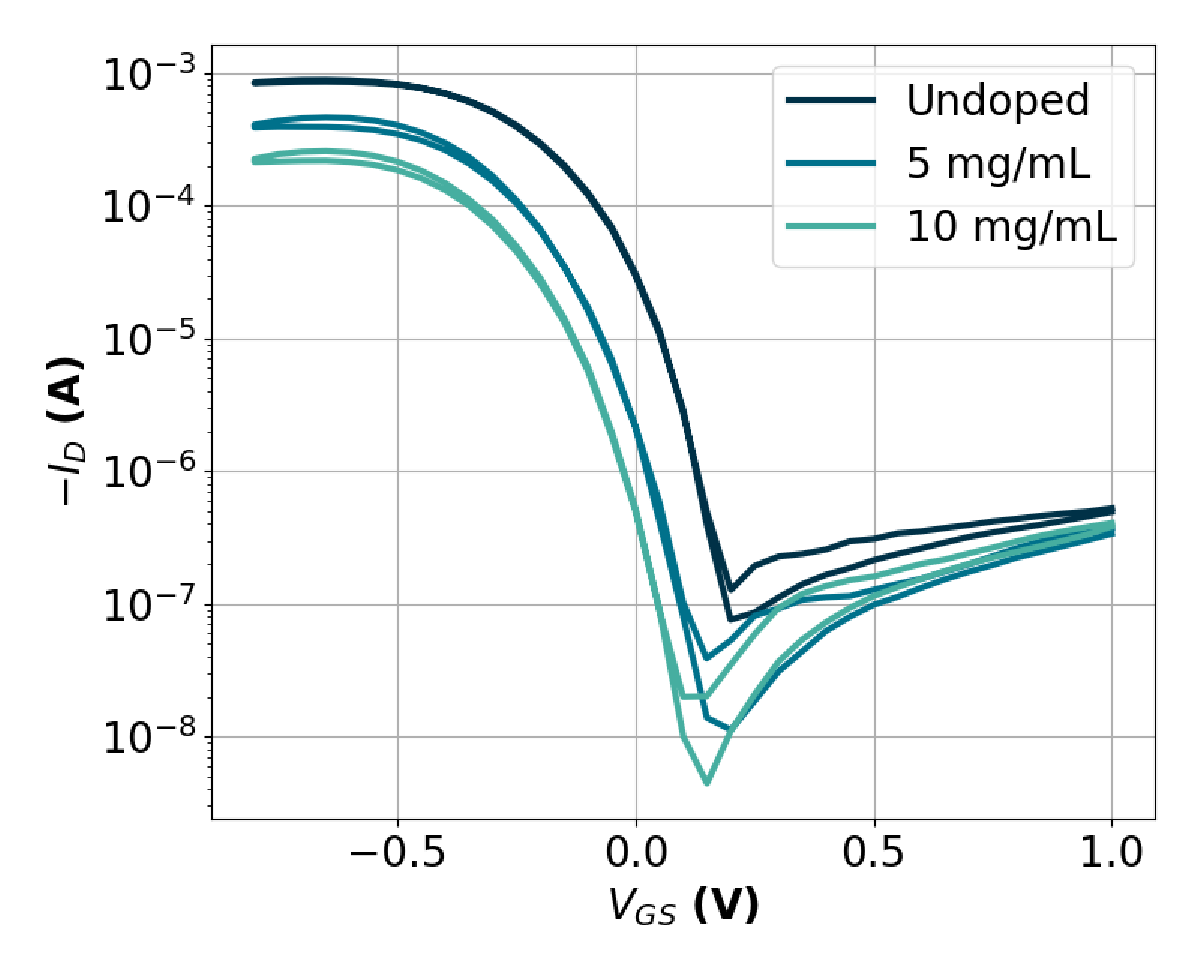
\includegraphics[width=7cm]{Images/pdf/Shift_Vds3.pdf} }
    %\qquad
    %\sidesubfloat[]{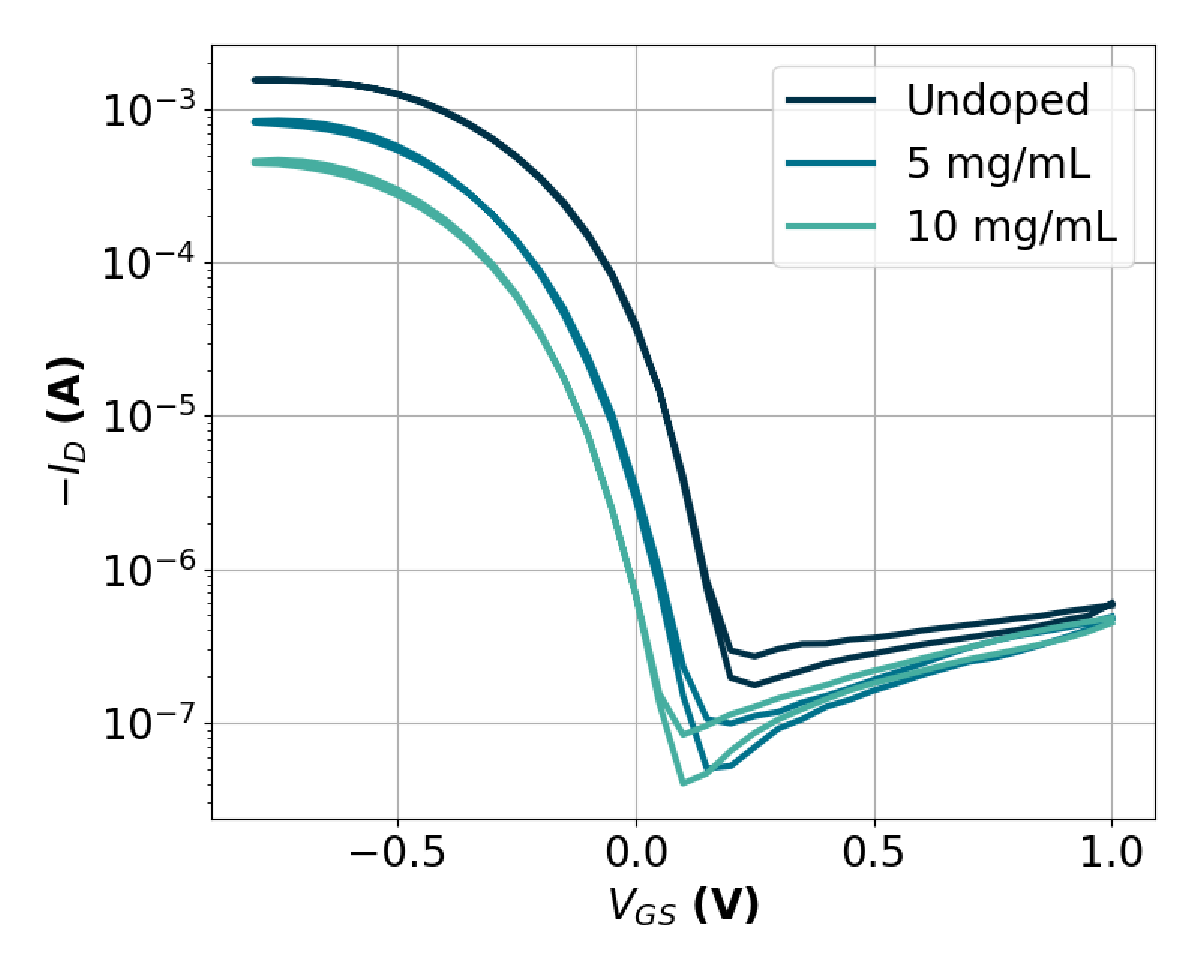
\includegraphics[width=7cm]{Images/pdf/Shift_Vds5.pdf}}
    %\sidesubfloat[]{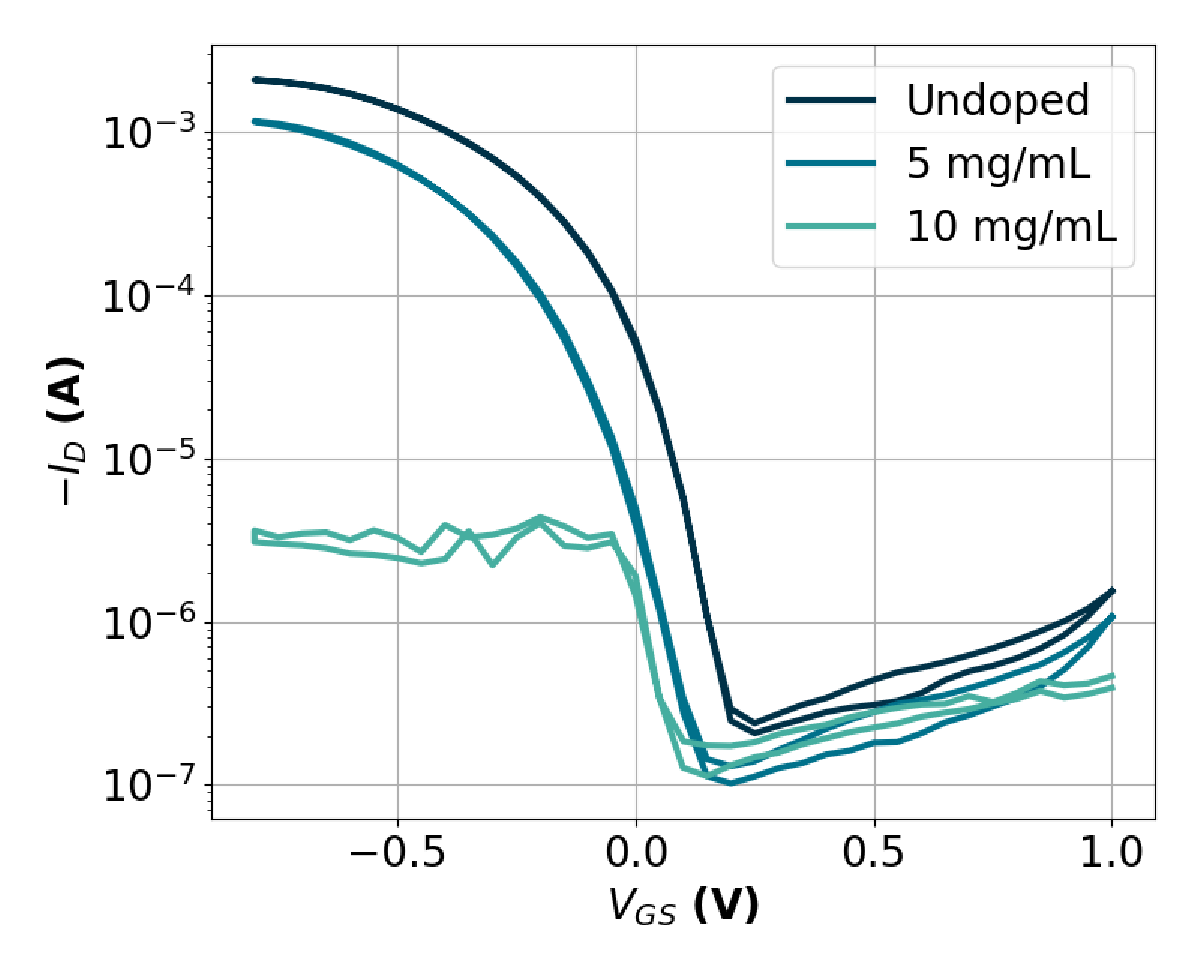
\includegraphics[width=7cm]{Images/pdf/Shift_Vds7.pdf} }
    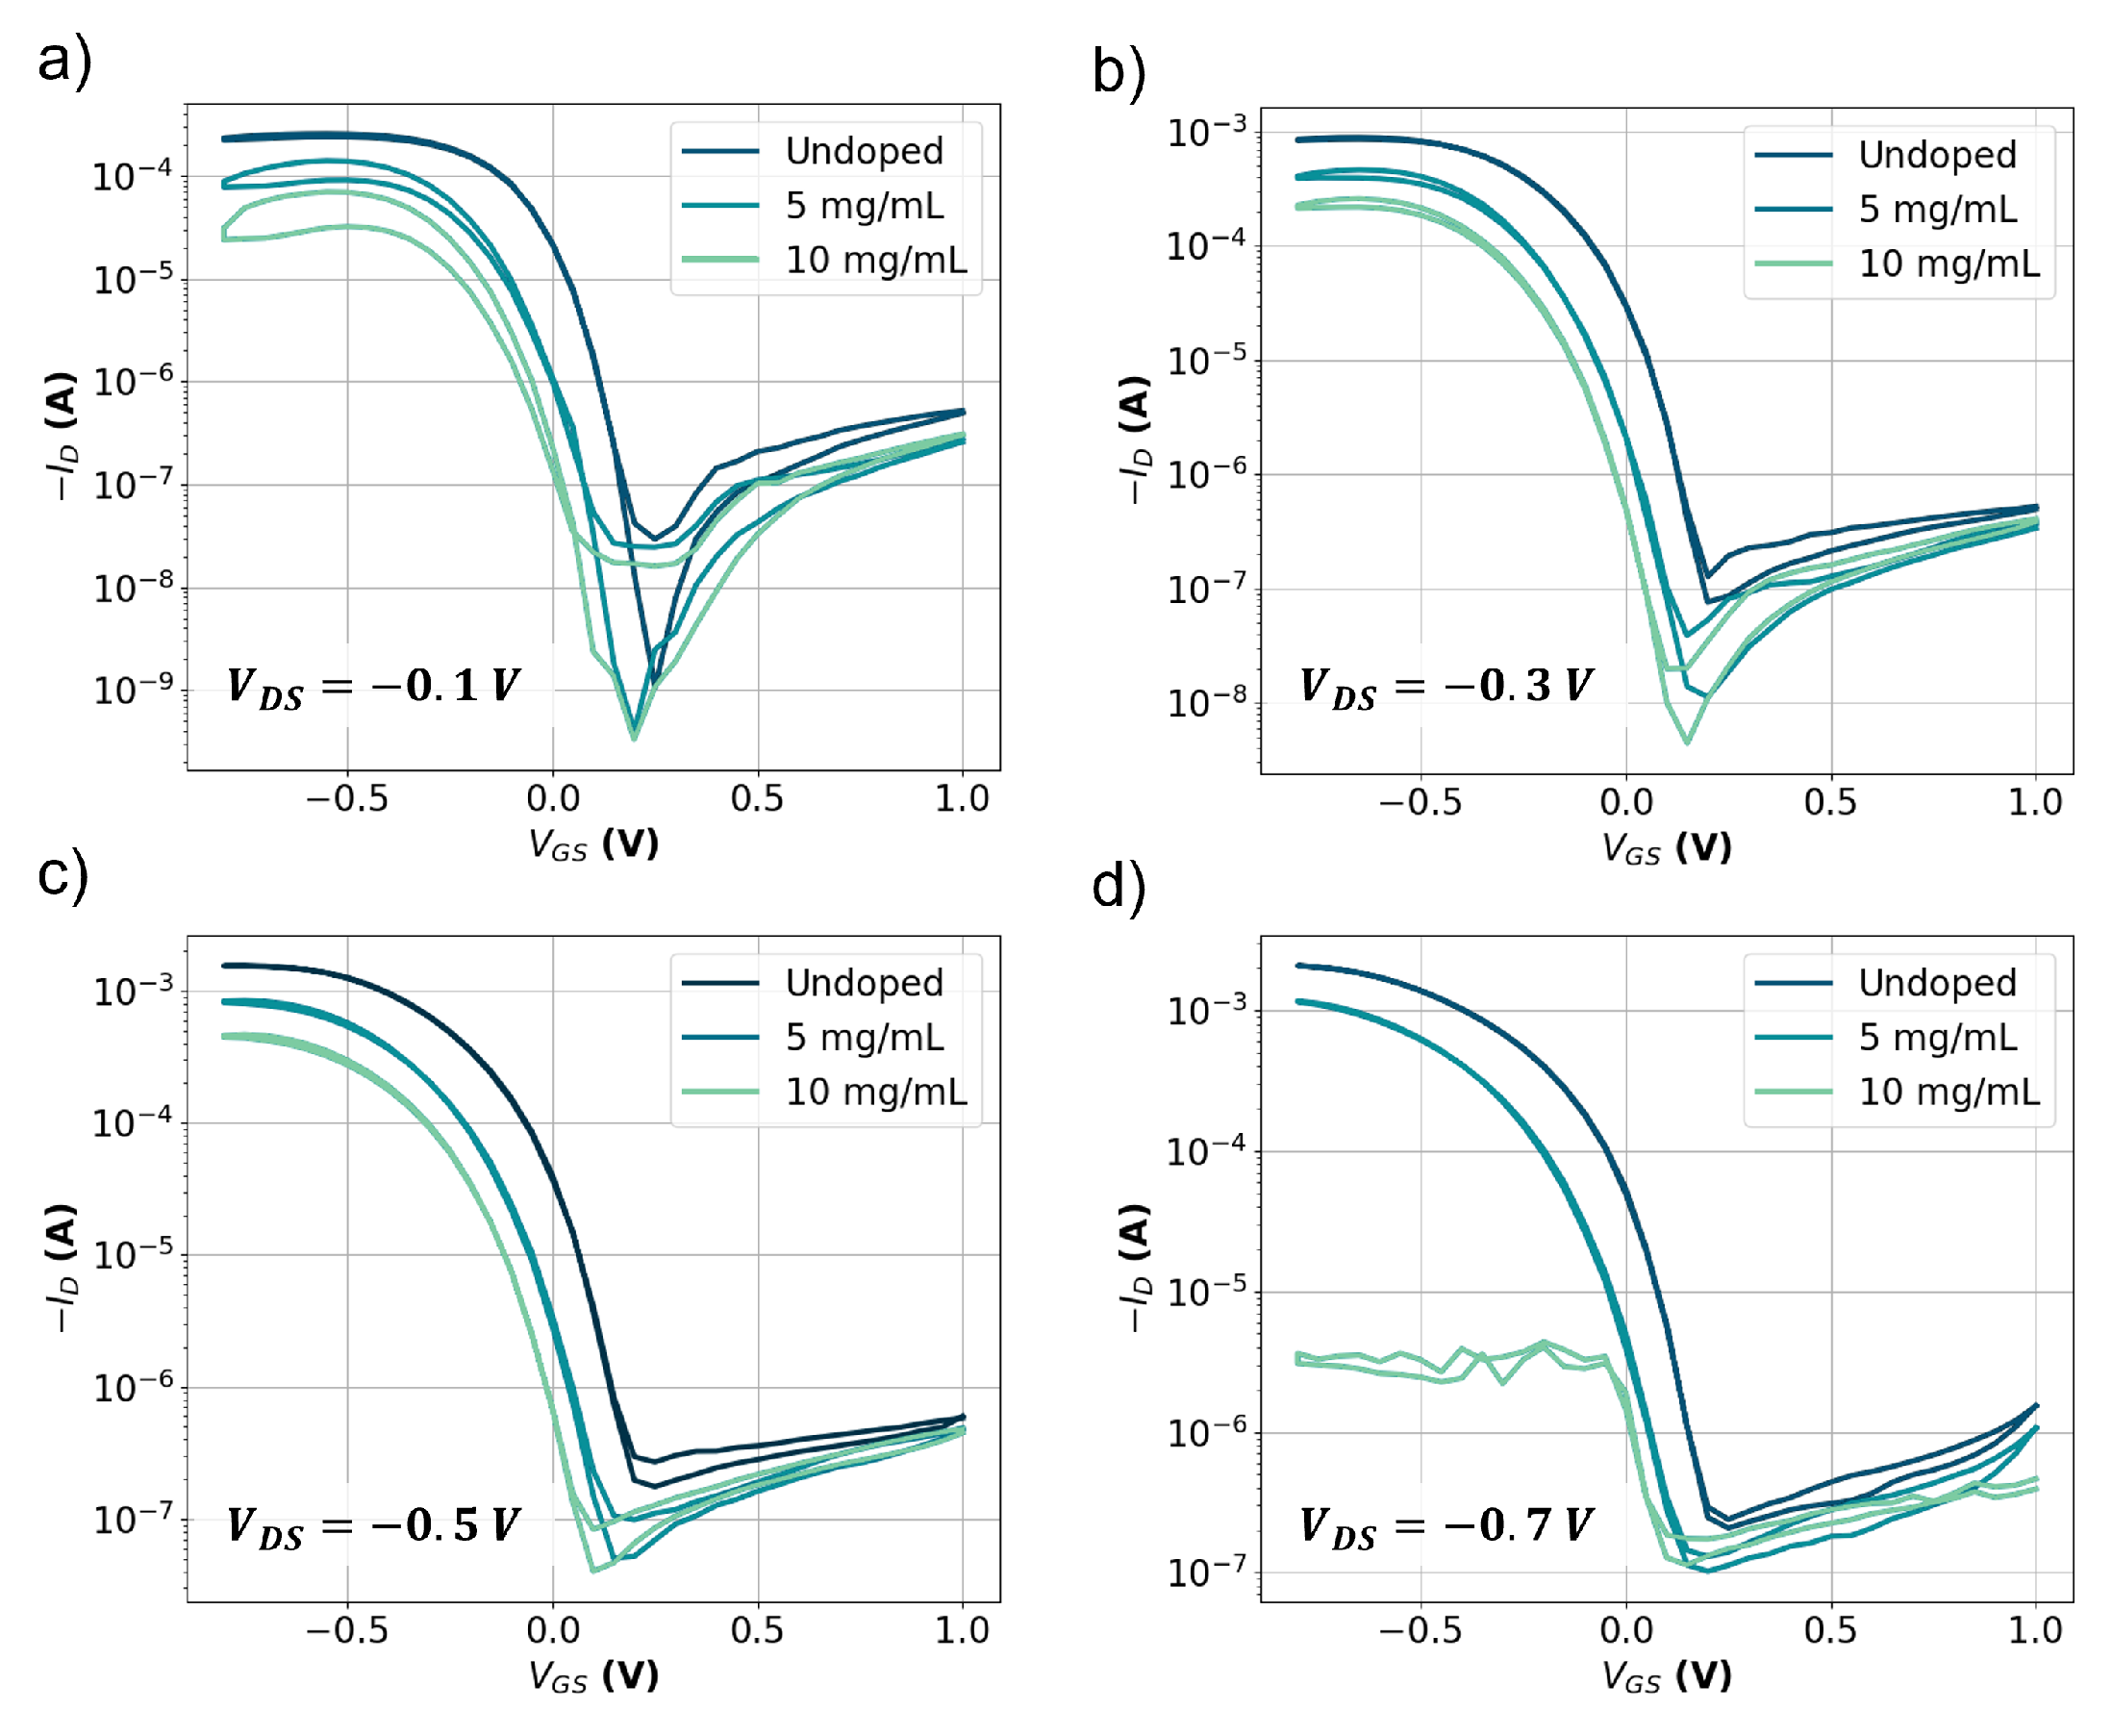
\includegraphics[width=\textwidth]{Images/pdf/Trans_doping.pdf}
    \caption[Transfer characteristics comparing different doping levels]{Transfer characteristics comparing undoped, 5 mg/mL and 10 mg/mL dopants devices, each graph represent a different $V_{DS}$}
    \label{fig:shift1}
\end{figure}

Figure \ref{fig:shift1} illustrates that doped devices exhibit minimal differences in $I_{D,OFF}$ but  there is a noticeable decrease in $I_{D,ON}$ as the doping levels increase. This is reflected in the maximum transconductance values displayed in Table \ref{tab:trans}, where a clear drop of |$g_{m,max}$| is evident with increasing doping levels. This outcome aligns with our initial hypothesis and warrants further investigations with impedance measurements to calculate volumetric capacitance. %, since as explained in the Background chapter, Section \ref{subsec:devphy}, $I_{D}$ depends on this values along with the charge carrier mobility.

%When doping our polymer, we are increasing its conductivity by inducing new charges in its backbone, however, the introduction of new ionic species will negatively impact the mobility of the induced charges, which explains the decrease in $I_{D,ON}$. %????

However, a more striking observation is evident in Figure \ref{fig:shift1} and Figure \ref{fig:vth_vds}: the turn-on voltages and threshold voltages, respectively, \textbf{have shifted towards negative values} as the dopant concentration increased in all $V_{DS}$ values, \textbf{contradicting our initial hypothesis}. This suggest a kind of \textbf{``compensation doping effect''} in the OECTs, which requires further investigation and resolution. %, and as explained in the Background chapter, p(g3T2-T) as a type VI OMIEC, unlike PEDOT:PSS, have ionic species as free carriers and not chemically bonded. Further analysis in the conductivity needs to be done to understand to impact of this coupling in our undoped and doped polymer.
%% EG3 ensure no cation trapping in the crystalline phase of OMIECs

Additionally, threshold voltage values exhibited lower variability among different $V_{DS}$ values with higher doping levels, are despicted in Figure \ref{fig:vth_vds}a.  In the undoped device, the variability could be attributed to the ORR, which may differ under different drain bias conditions. In contrast, in the doped devices, this variability is expected to decrease since doping depletes reactive electrons from p(g3T2-T) with F$_{4}$TCNQ, ensuring better stability in air \cite{tanTuningOrganicElectrochemical2022}. %Further analysis needs to be done to confirm this hypothesis.  %Then although we are impacting mobility and repeatability among loops, the values at different drain biased are maintain. 

\begin{figure}[ht]
  \centering
  %\sidesubfloat[]{{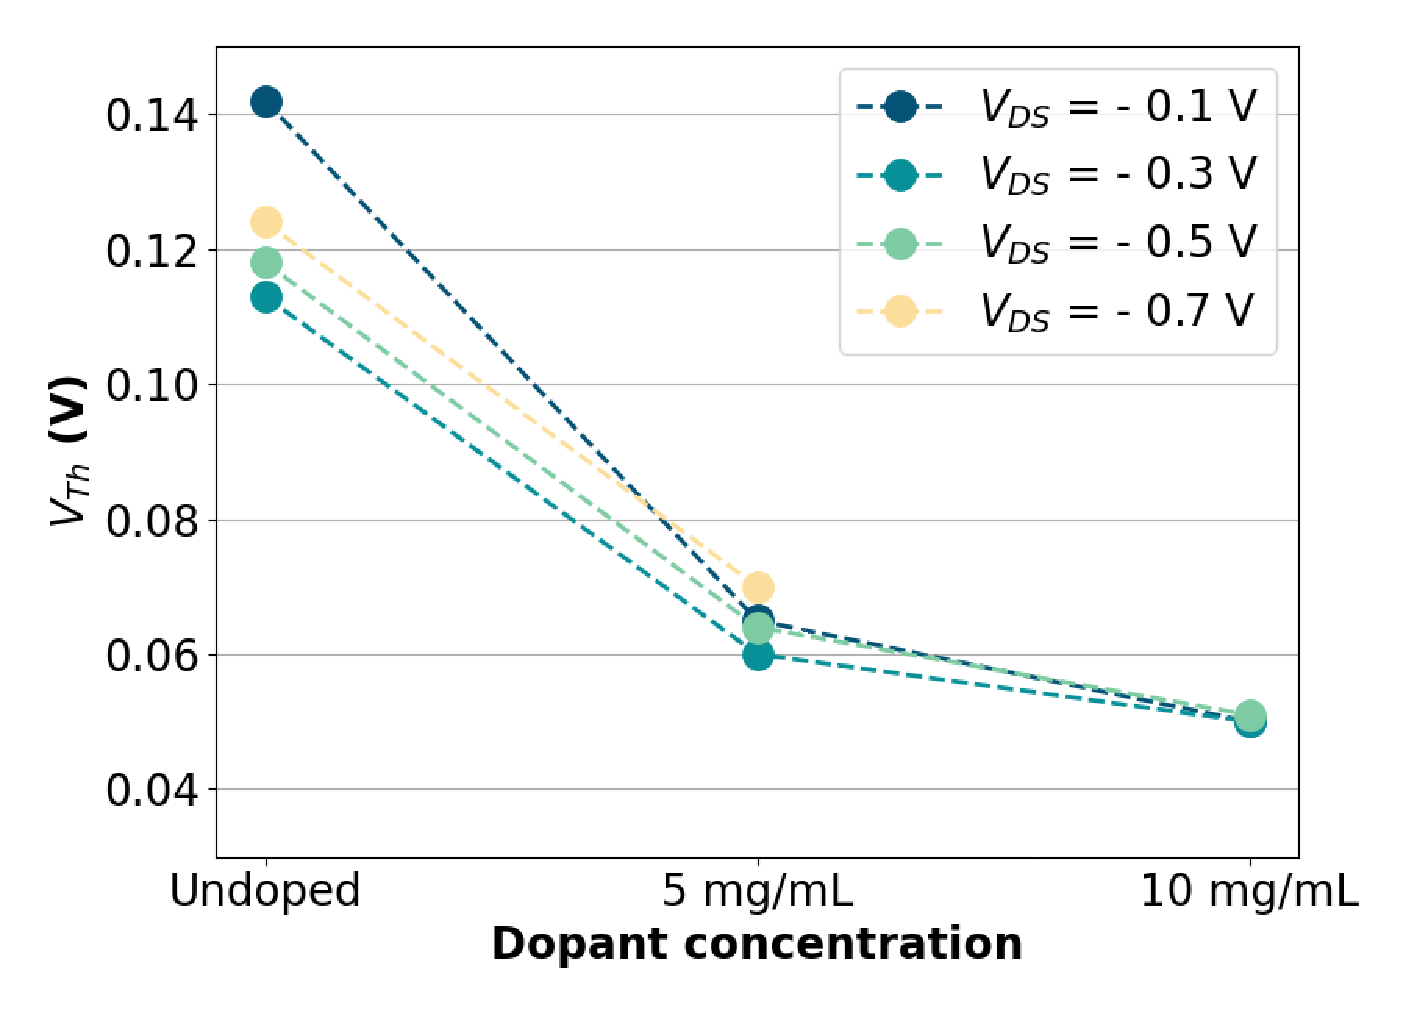
\includegraphics[width=7cm]{Images/pdf/vth_shift_vds.pdf} }}
  %\sidesubfloat[]{{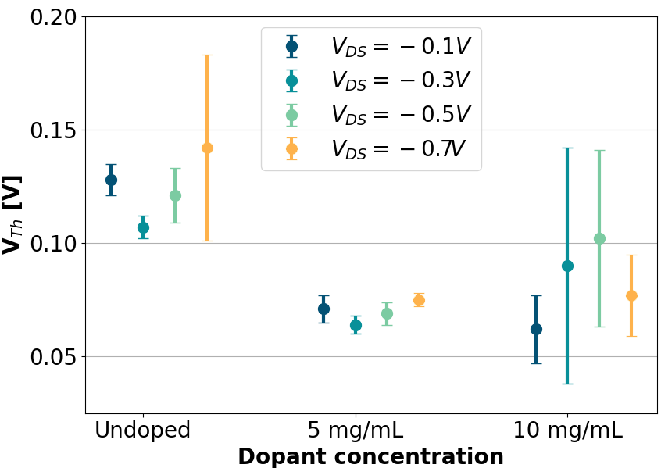
\includegraphics[width=7cm]{Images/pdf/vth_shift_2.pdf} }}
  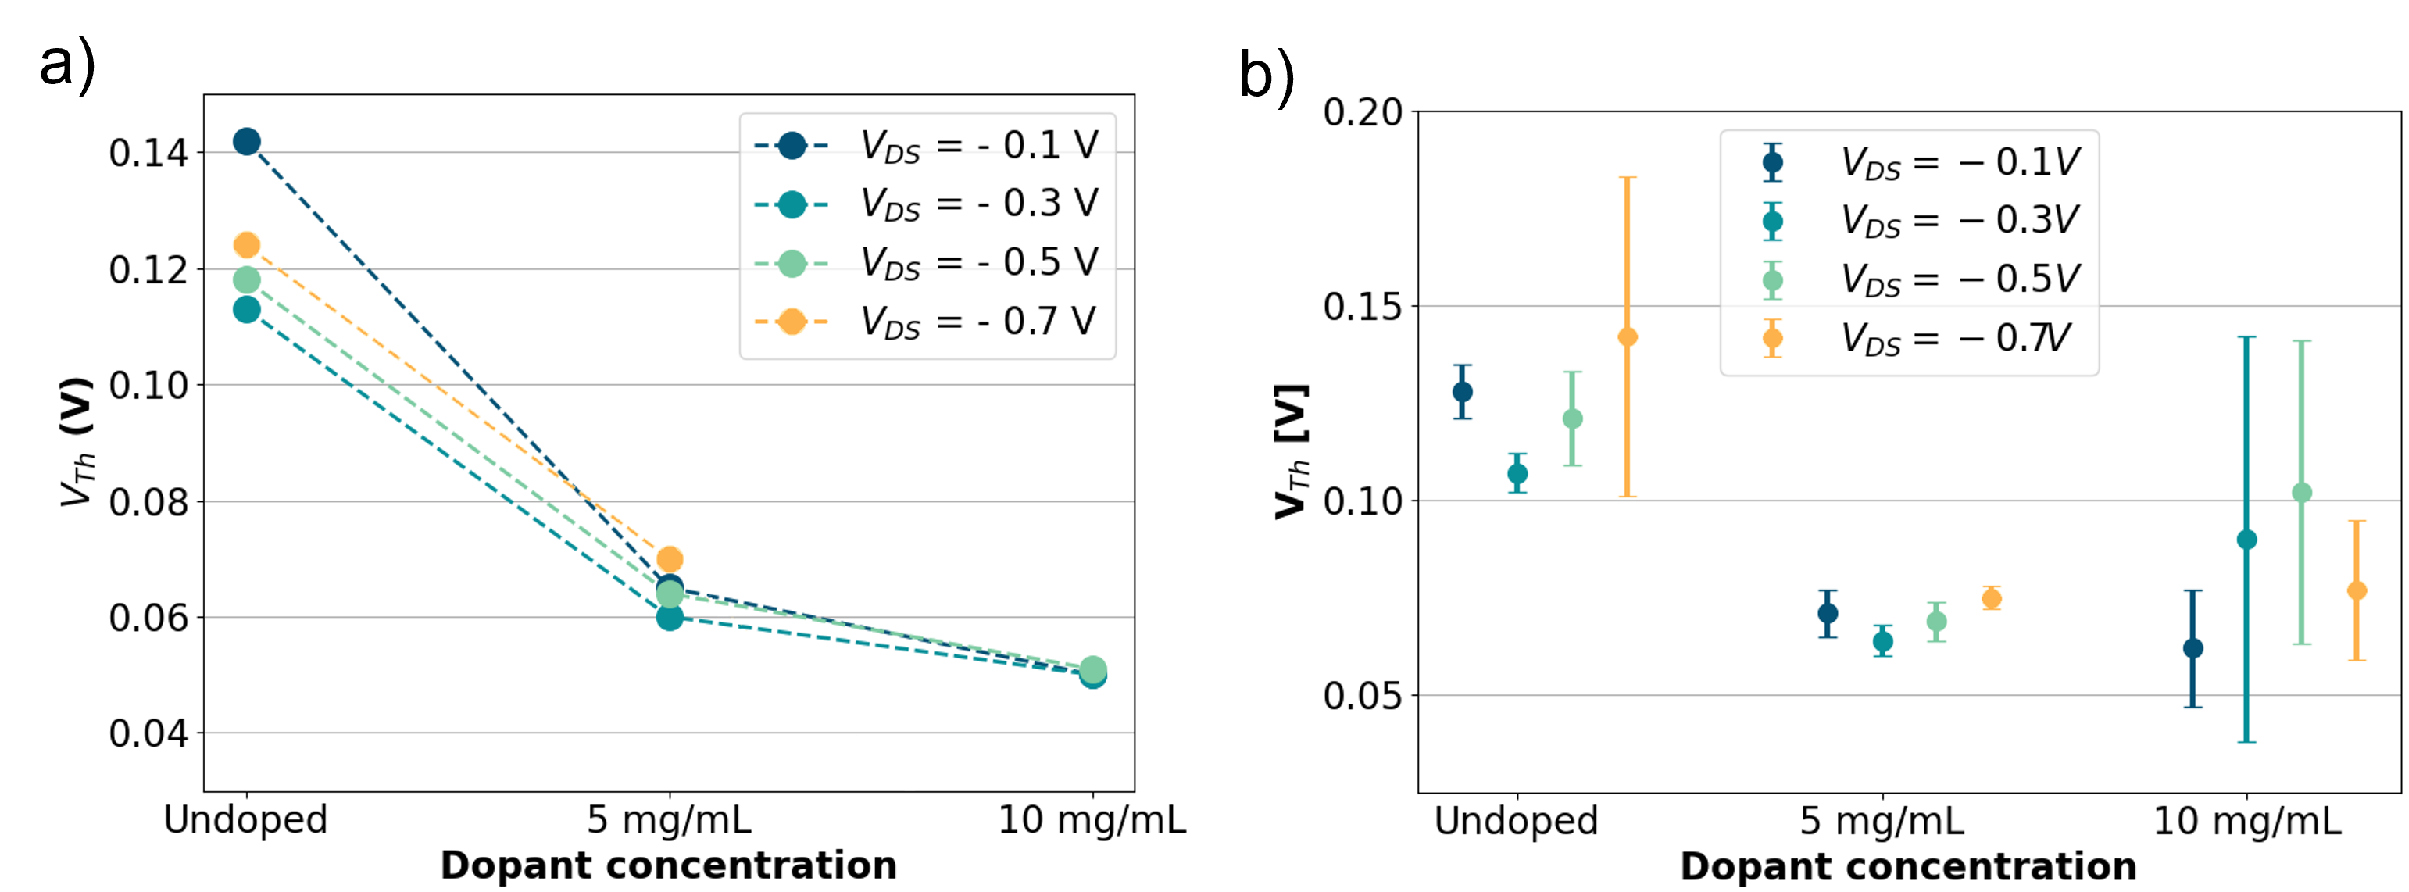
\includegraphics[width=\textwidth]{Images/pdf/vth_shift_channel.pdf} 
  \caption[Threshold shift at different doping levels and $V_{DS}$]{Threshold shift at different doping levels and $V_{DS}$ corresponding to a) data shown in Figure \ref{fig:transx2}, and b) all operating devices in each sample.}
  \label{fig:vth_vds}
\end{figure}

However, the statistical analysis presented in Figure \ref{fig:vth_vds}b aligns with the previous statement for 5 mg/mL dopant concentration only, but not for 10 mg/mL. Some other factors may have intervened such as low degree of homogeneity in doping or patterning defects.

Furthermore, while not presented in this report, it was observed during the analysis that undoped OECT devices exhibit higher repeatability in transfer characteristics as measurement loops increase. The saturation of ORR in undoped species, as mentioned earlier, may contribute to this repeatability. However, the variability in doped species requires further study. For instance, understanding the stability of dopants upon contact with the polymer and the electrolyte would be valuable. %Potential for appendix
%but it is yet unclear. %An new hypothesis that could explained is to consider our environmental conditions as a infinite reservoir of molecular oxygen, until this unwanted doping and ORR reaches saturation, making it stable. In the case of F$_{4}$TCNQ, stability is still unclear and further investigation will be done in the next sections.

\subsection{Stability of Undoped and Doped p(g3T2-T)} \label{subsec:stab}
%\subsection{Stability on Air of p(g3T2-T)}
From the previous subsection, it was concluded that a better understanding of the stability of undoped and doped p(g3T2-T) under ambient conditions, as well as how their electrical properties change upon contact with the SSE precursor, is needed. Consequently, this subsection will focus on monitoring the channel conductivity under both $N_{2}$ and ambient environments, both before and after contact of SSE precursor.

The channel conductivity of an undoped device was measured immediately after spin-coating, yielding a value of 1 $\mu$S. After undergoing the patterning process described in the previous sections, the conductivity increased three orders of magnitude to approximately 1 mS. Even though, $\mu$S values already signify oxidation, the patterning process further oxidizes our material. %In this section, a way to revert this oxidation and find a compatible process to obtain accumulation-mode OECTs.
%Before getting into the revers

Measurements of $I_{D}$ at $V_{DS}$ of -0.3 V and no gate bias exhibited a small decrease of 4\% and small increase of 15\% within two hours in $N_{2}$ and ambient air environments, respectively. This observation suggests that stability in ambient air is compromised due to unwanted doping.

A similar study was conducted with a doped device containing 5 mg/mL of F$_{6}$TCNNQ dopant, resulting a higher level of doping compared to F$_{4}$TCNQ at the same concentration, as detailed in Appendix \ref{app:abs}. The channel conductivity reached a value of 266 $\mu$S with a reduction of 1.2\% within one hour in $N_{2}$ environment and remained stable with minimal fluctuations of 1.0\% within one hour in ambient condition. This indicates a lower conductivity compared to the oxidized p(g3T2-T) but similar stability in air, as expected from reference \cite{tanTuningOrganicElectrochemical2022}.

Remarkably, upon contact with SSE precursor, conductivity of both samples drops significantly, approximately six orders of magnitude, in an $N_{2}$ environment, reaching the sensitivity limits of our equipment and resulting in a noisy signal, as shown in Figure \ref{fig:revox1}a. One plausible explanation is that p(g3T2-T), as a type VI OMIEC, lacks chemical binding with TCNQ$^{-}$ anions. When in contact with the electrolyte, the anions are drawn away from the polymer backbone (de-doping), restoring its original insulating state. However, it may be possible that cations from the electrolyte could enter the polymer film and neutralize the anions. Further experiments would be needed to clarify both explanations. Either way, having an insulating polymer film is essential for accumulation-mode OECTs.
%\begin{table}[ht]
%\centering
%\caption{Conductivity measurements of undoped p(g3T2-T)}
%\begin{tabular}{l|c}
%Condition  & Conductivity (S) \\\hline
%Unpatterned & 1.3 $\times$ 10^{-6} \\
%Patterned & 1.0 $\times$ 10^{-3} \\
%\end{tabular}
%\label{tab:cond}
%\end{table}

\begin{figure}[ht]
    \centering
    %\subfloat[]{{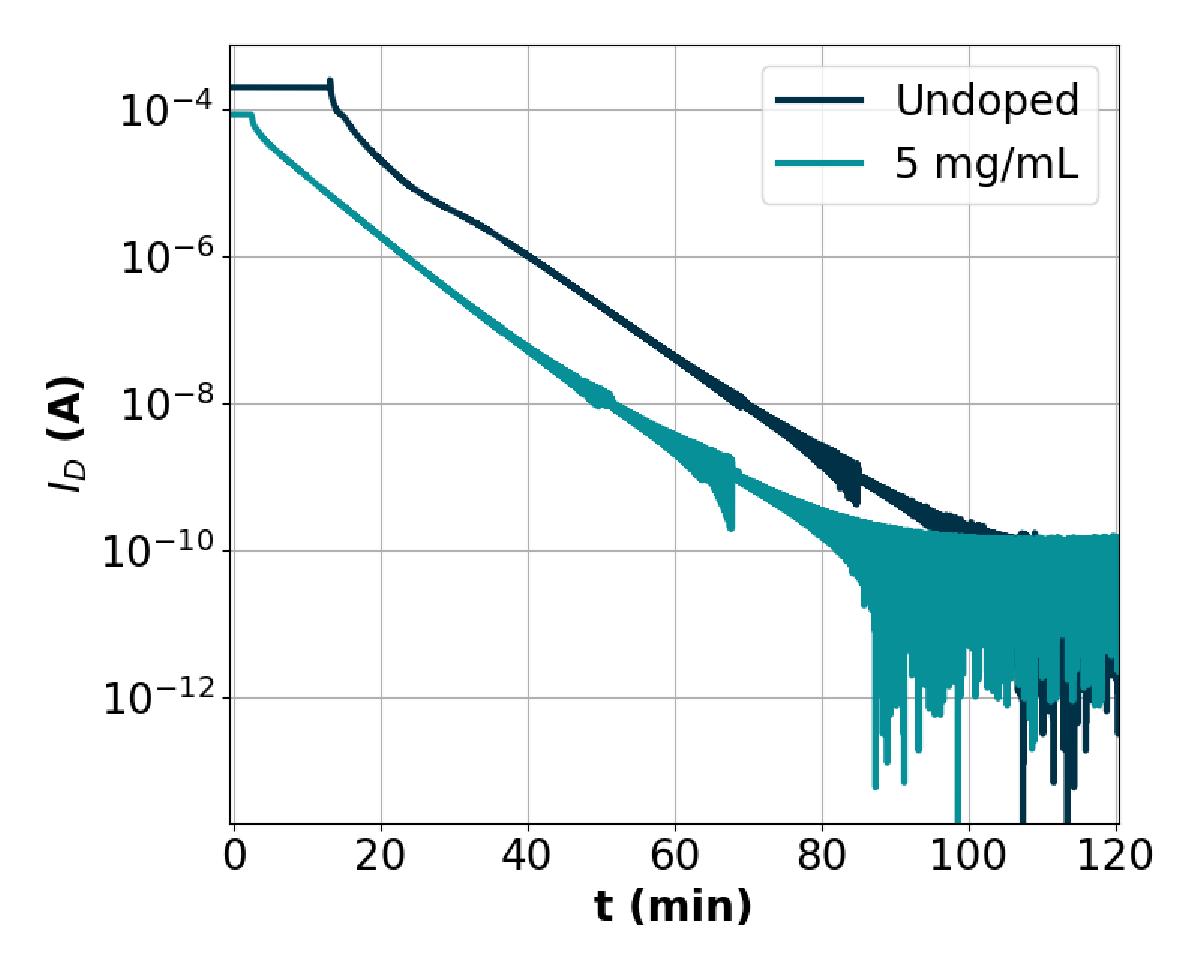
\includegraphics[width=7cm]{Images/pdf/revox_gb_only.pdf} }}
    %\qquad
    %\subfloat[]{{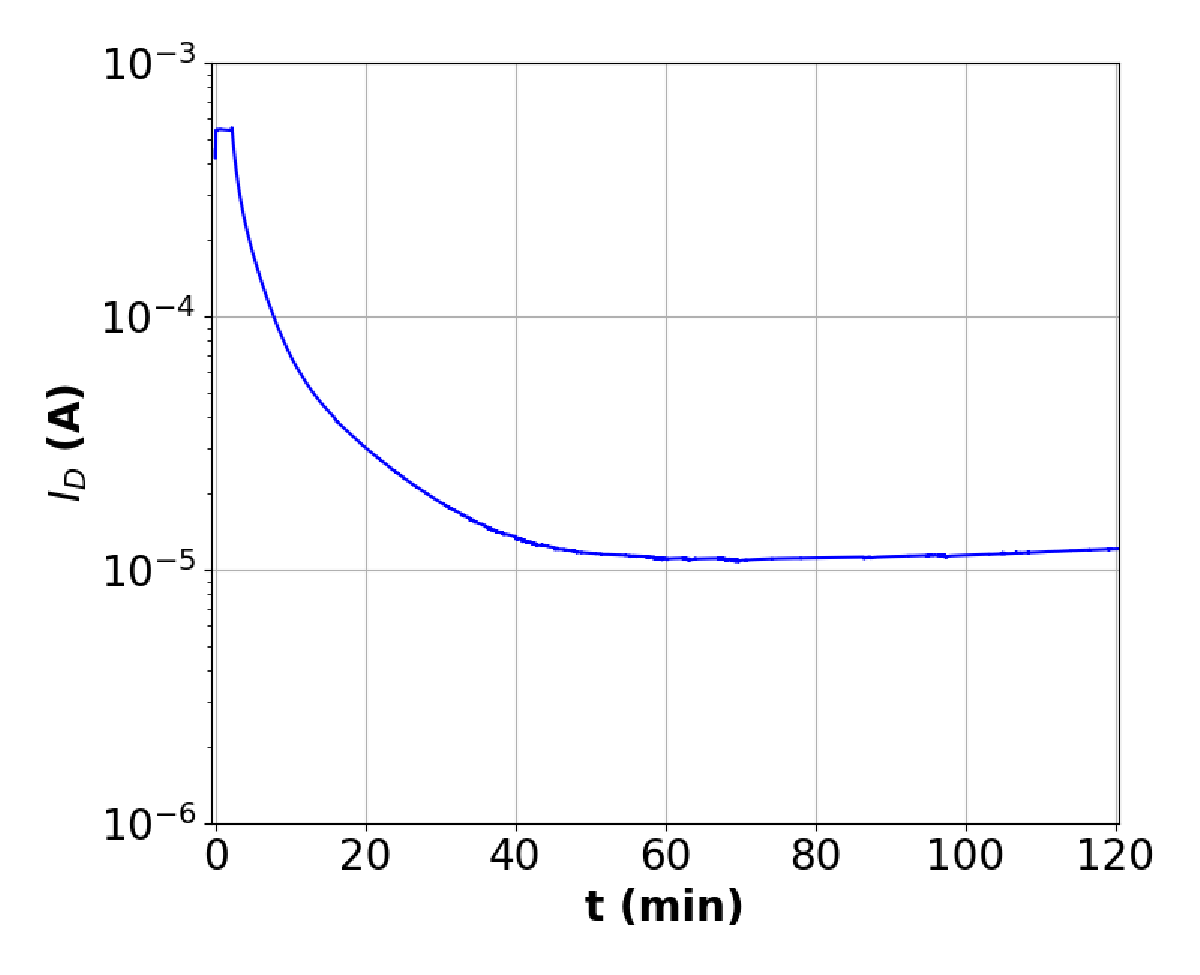
\includegraphics[width=7cm]{Images/pdf/revox_air.pdf} }}
    %\subfloat[Ambient and $N_{2}$ environment]{{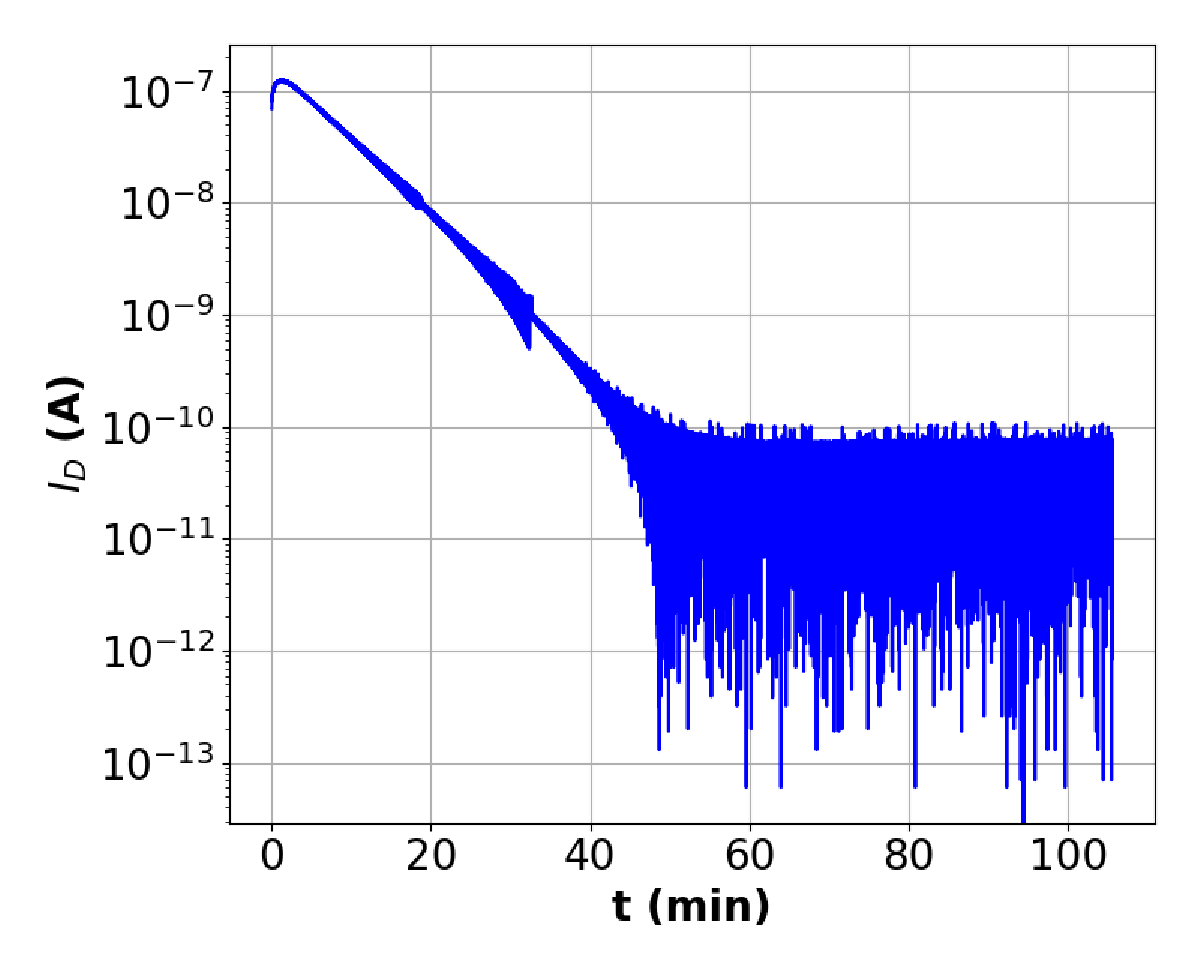
\includegraphics[height=5.5cm]{Images/pdf/revox_gb_afterair.pdf} }}
    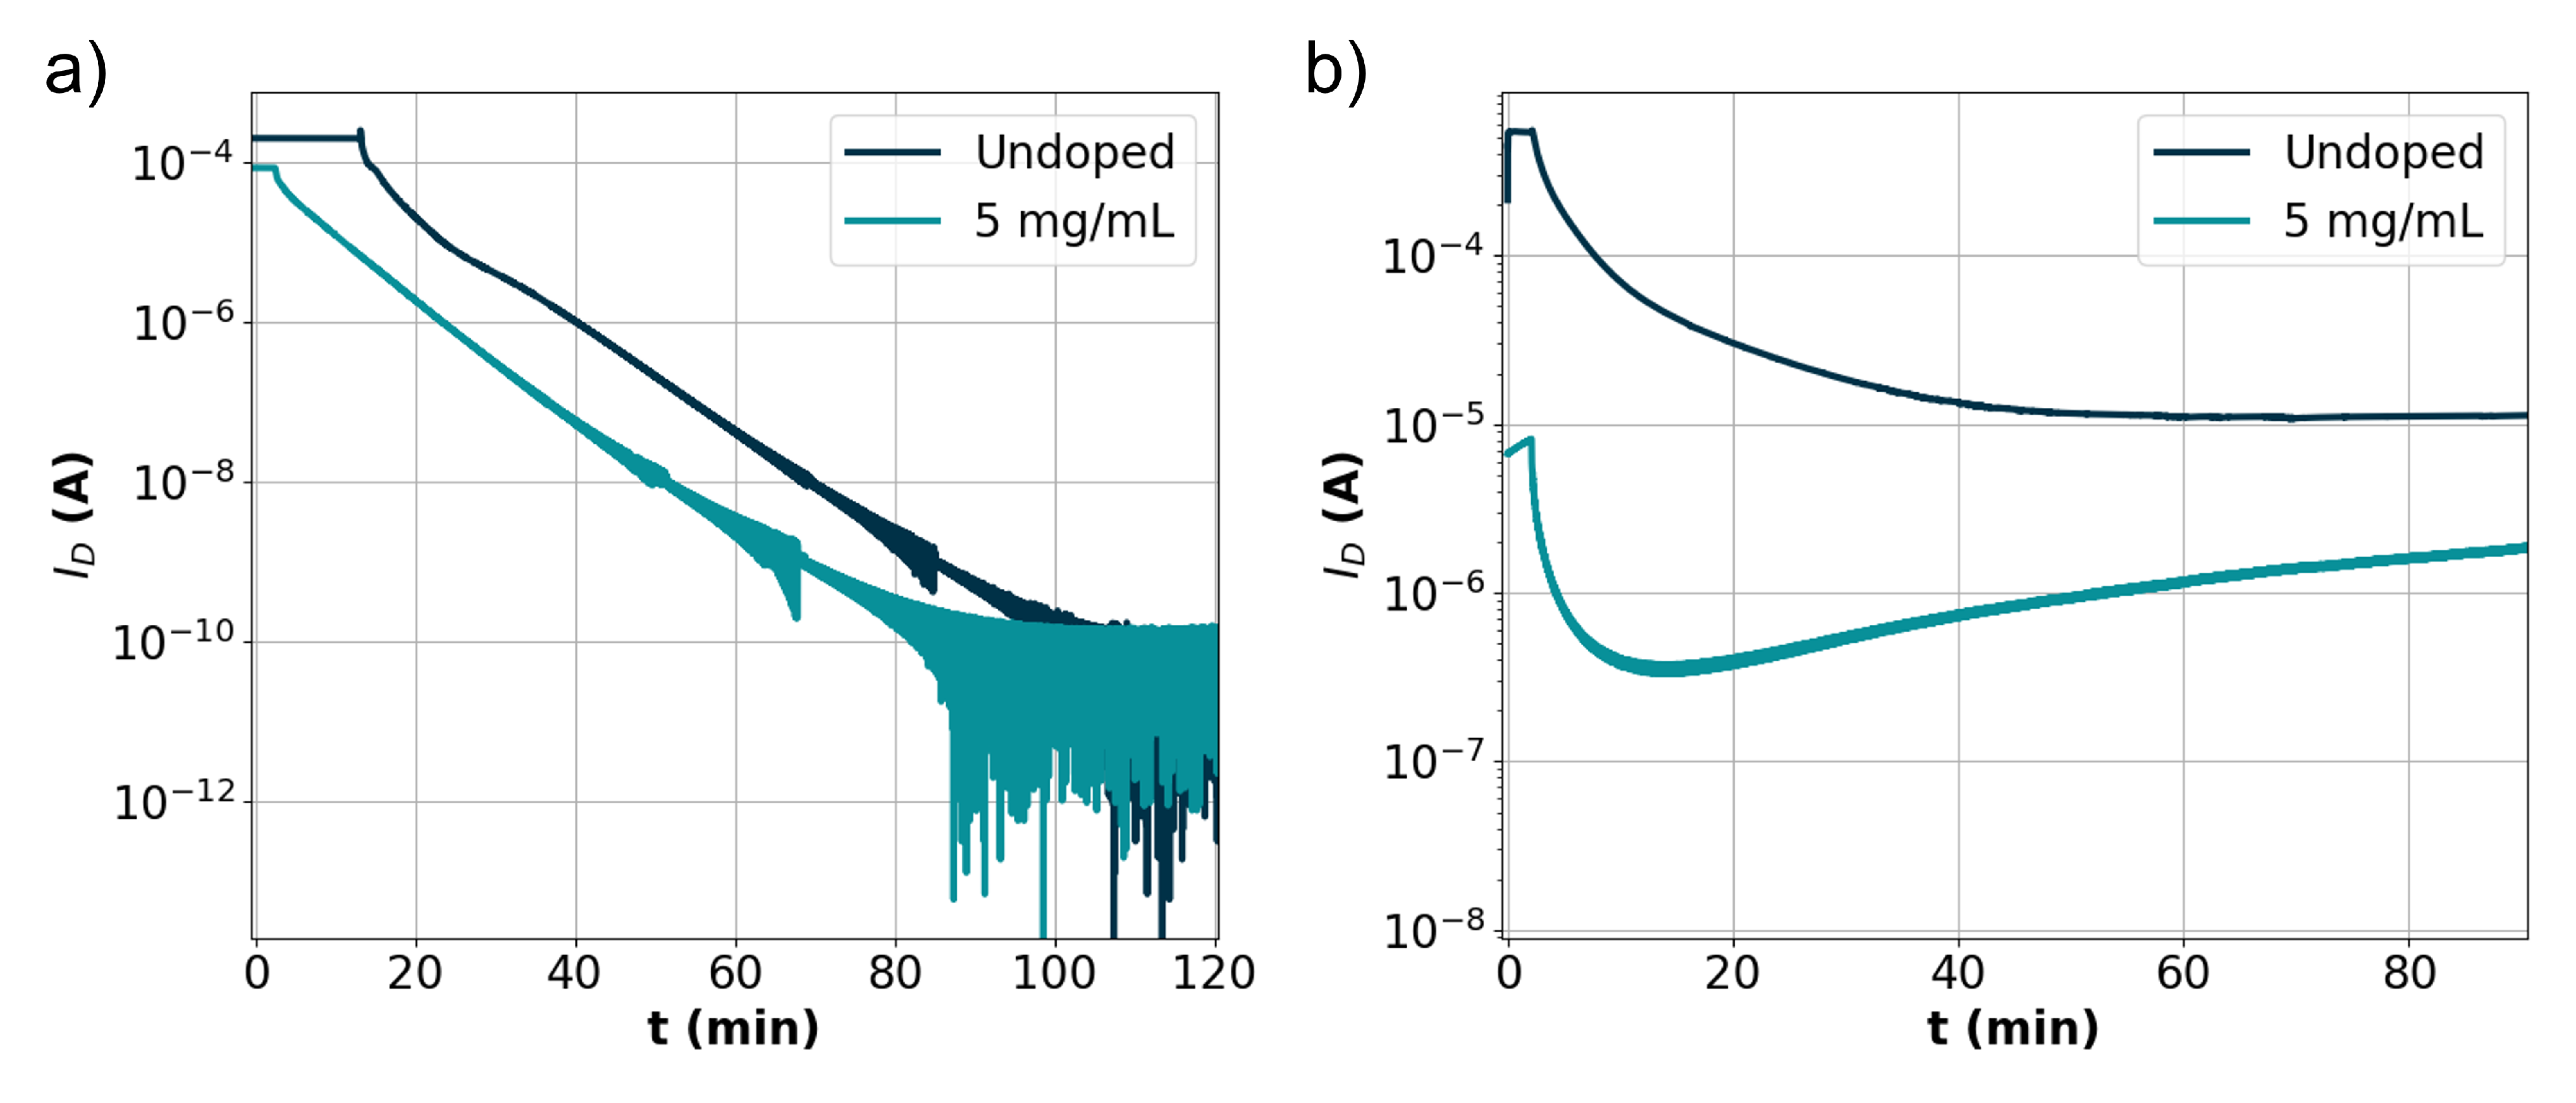
\includegraphics[width=\textwidth]{Images/pdf/stability.pdf}
    \caption[Drain current over time of undoped-p(g3T2-T) coupled with SSE precursor]{Drain current over time of undoped p(g3T2-T) coupled with SSE precursor under a) $N_{2}$, and b) ambient environment%, C)$N_{2}$ environment after B)
    .}
    \label{fig:revox1}
\end{figure}

Under ambient conditions, there is a smaller decrease of slightly more than one order of magnitude for the undoped sample, as seen in Figure \ref{fig:revox1}b. The doped sample initially exhibited a similar but faster drop within the first 15 minutes, followed by a sudden increase of $I_{D}$. In both scenarios, the ORR prevented a greater decrease in current. The fluctuation seen in the doped species may be attributed to the simultaneous occurrence of irreversible de-doping %$TCNQ^{-}$ anions
and ORR . %Another undoped sample share the same results.

Transfer curves of the undoped device using an Ag/AgCl pellet as gate were measured under ambient conditions after de-doping in $N_{2}$ environment, as despicted in Figure \ref{fig:transrevox1}. The device exhibited shifts in its ON voltage and negative threshold voltages values, as summarized in Table \ref{tab:vth_air}, moving towards negative values. A visible sign of degradation was perceived at the end of the measurements (in this case, when $V_{DS}$ was -0.1 V). This will be further addressed in the next subsection.

\begin{figure}[ht]
    \centering
    %\subfloat[N$_{2}$ environment]{{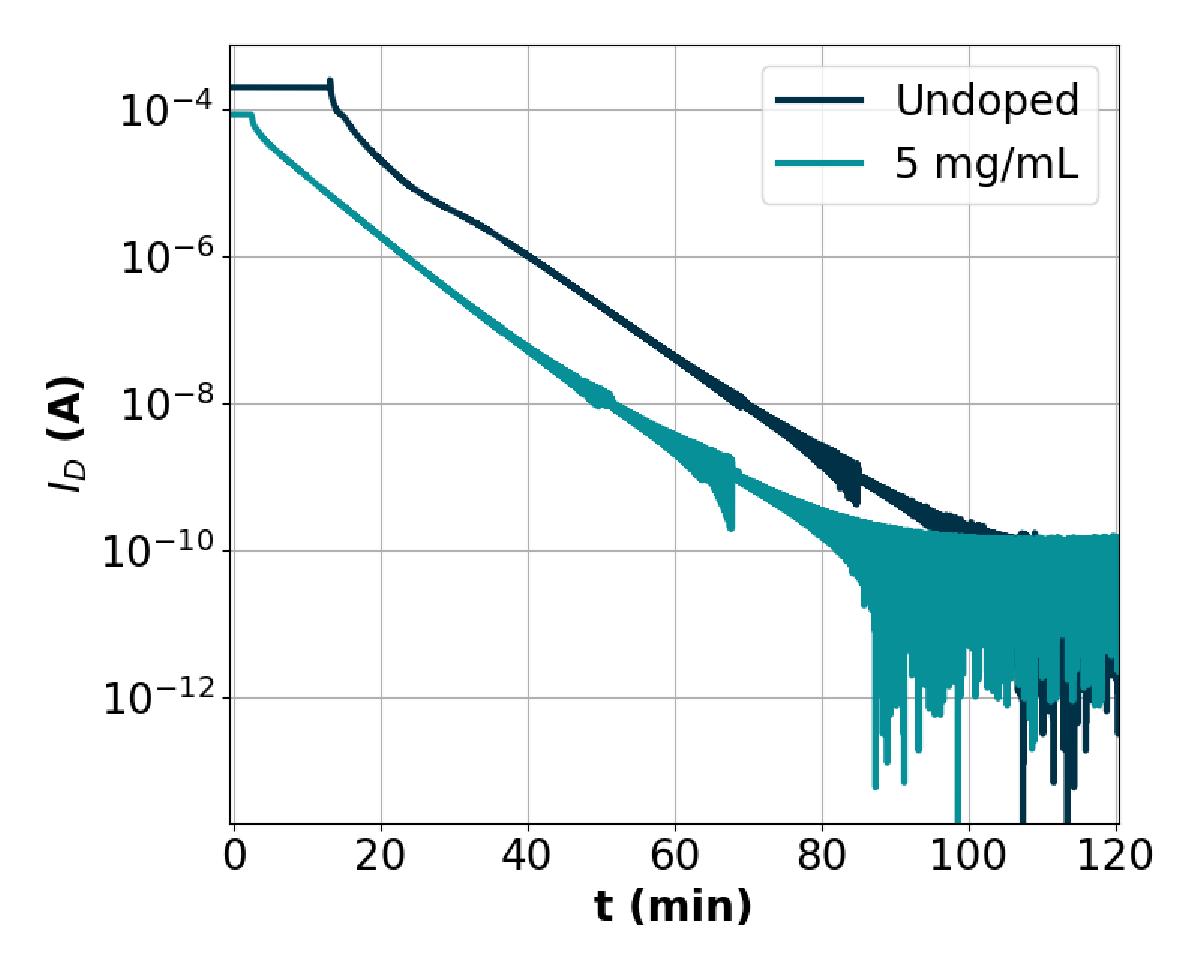
\includegraphics[width=5.5cm]{Images/pdf/revox_gb_only.pdf} }}
    %\subfloat[Transfer in ambient]{{
    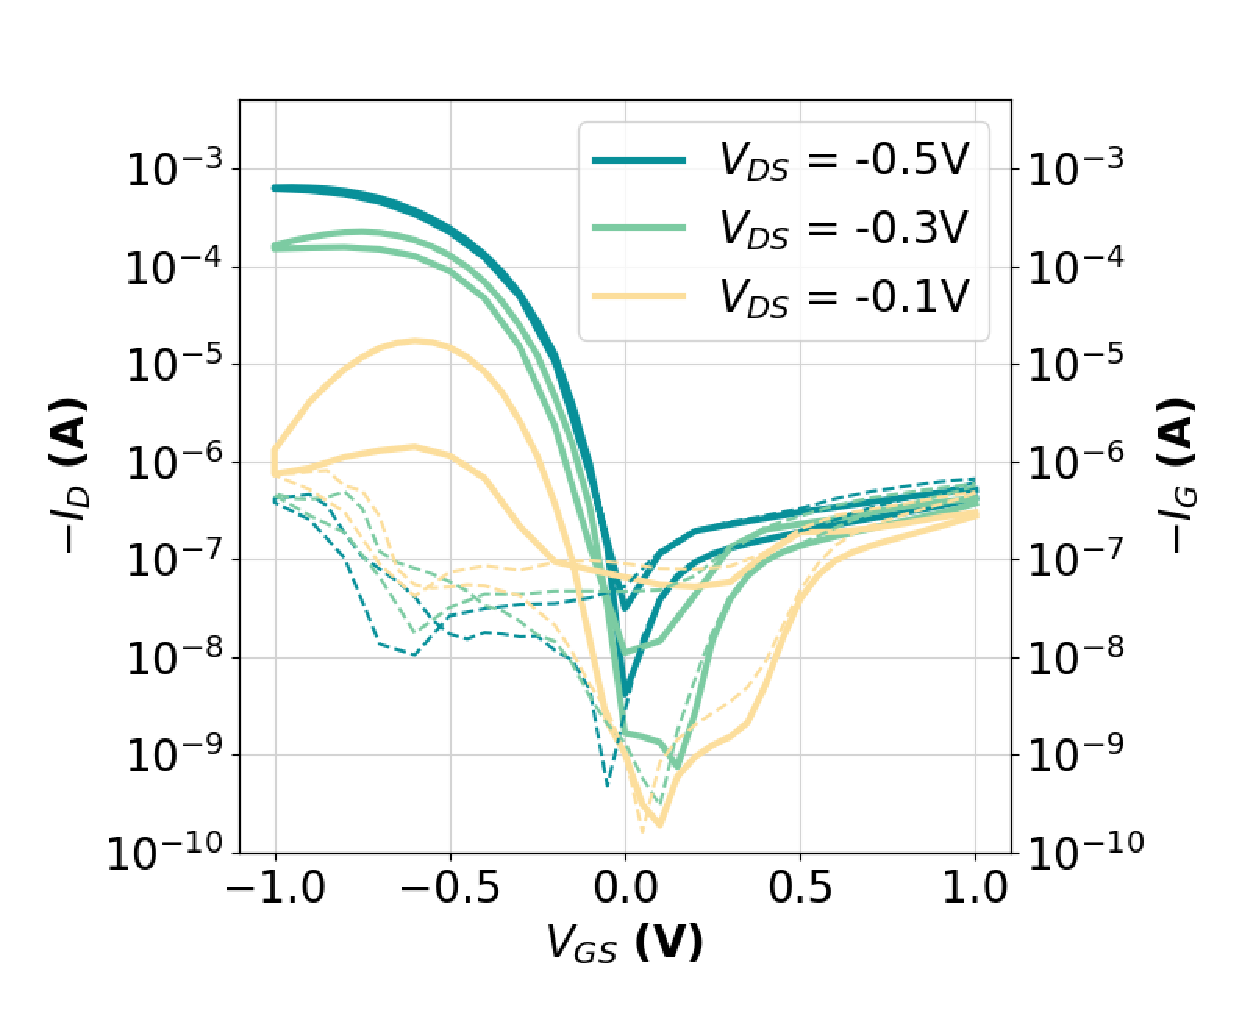
\includegraphics[width=7.5cm]{Images/pdf/revox_transfer_loop2.pdf}% }}
    \caption[Transfer characteristics after electrochemical de-doping]{Transfer characteristics after electrochemical de-doping at different $V_{DS}$ under ambient conditions. Solid and dashed lines indicate $I_{D}$ and $I_{G}$, respectively.}
    \label{fig:transrevox1}
\end{figure}

\begin{table}[ht]
\centering
\caption{Threshold voltage extracted from Figure \ref{fig:transrevox1}}
\begin{tabular}{c|c}
 $V_{DS}$ [V] & $V_{Th}$ [V] \\\hline
-0.1 & -0.18 \\
-0.3 & -0.15 \\
-0.5 & -0.13 \\ \hline
\end{tabular}
\label{tab:vth_air}
\end{table}

In summary, a pre de-doping step could potentially serve as a method for obtaining accumulation-mode OECTs by decreasing the conductivity of p(g3T2-T), and will be explored in the following section.

%\subsection{Reverse Oxidation of Undoped-p(g3T2-T)}
%\subsection{Counteracting Oxidation by Electrochemical De-doping} 
\subsection{Oxygen Reduction Reaction on OECTs} \label{subsec:revox}
Now that we have identified an alternative method to counteract the oxidation of p(g3T2-T), we will proceed with a preliminary study on oxygen reduction reaction in OECT using p(g3T2-T) channel and Ag/AgCl gate. Our first step will involve expediting the de-doping process by applying a positive gate bias to one of the devices. This will allow us to achieve low conductivity within a couple of minutes, as opposed to the two hours reported in the previous subsection. 

%It was observed that previous experiments took approximately two hours to fully de-dope p(g3T2-T) and reach minimal conductivity %an insulating state 
%in the polymer. However, this process could be expedited by applying .
%Additionally, the use of a high-temperature baking step to revert the oxidation of an p(g3T2-T) OECT %was a method suggested by colleagues in the Biosens group at IAPP and will also be tested.   
%\subsubsection{By Electrochemical Dedoping}
De-doping in a $N_{2}$ environment was performed by applying a +1 V gate bias. p(g3T2-T) reached its insulating state in less than 300 seconds, significantly faster than observed in the previous section. However, it was expected that this process would not be reversible upon disconnection of the gate. Figure \ref{fig:revox2}a confirms this expectation: after $I_{D}$ drastically dropped and the gate was disconnected (gray arrows), the current remained low, and leakage current is predominant. When the gate was reconnected (gold arrows), a capacitive current spike occurred but later stabilized to match the leakage current.
% Important commment from Rakesh: Did you try lower values? A high gate voltage would push the ions deeper into the channel and if the ions penetrate deep enough, the channel would shield them from flowing out after the gate voltage is removed.

\begin{figure}[ht]
    \centering
    \subfloat[]{{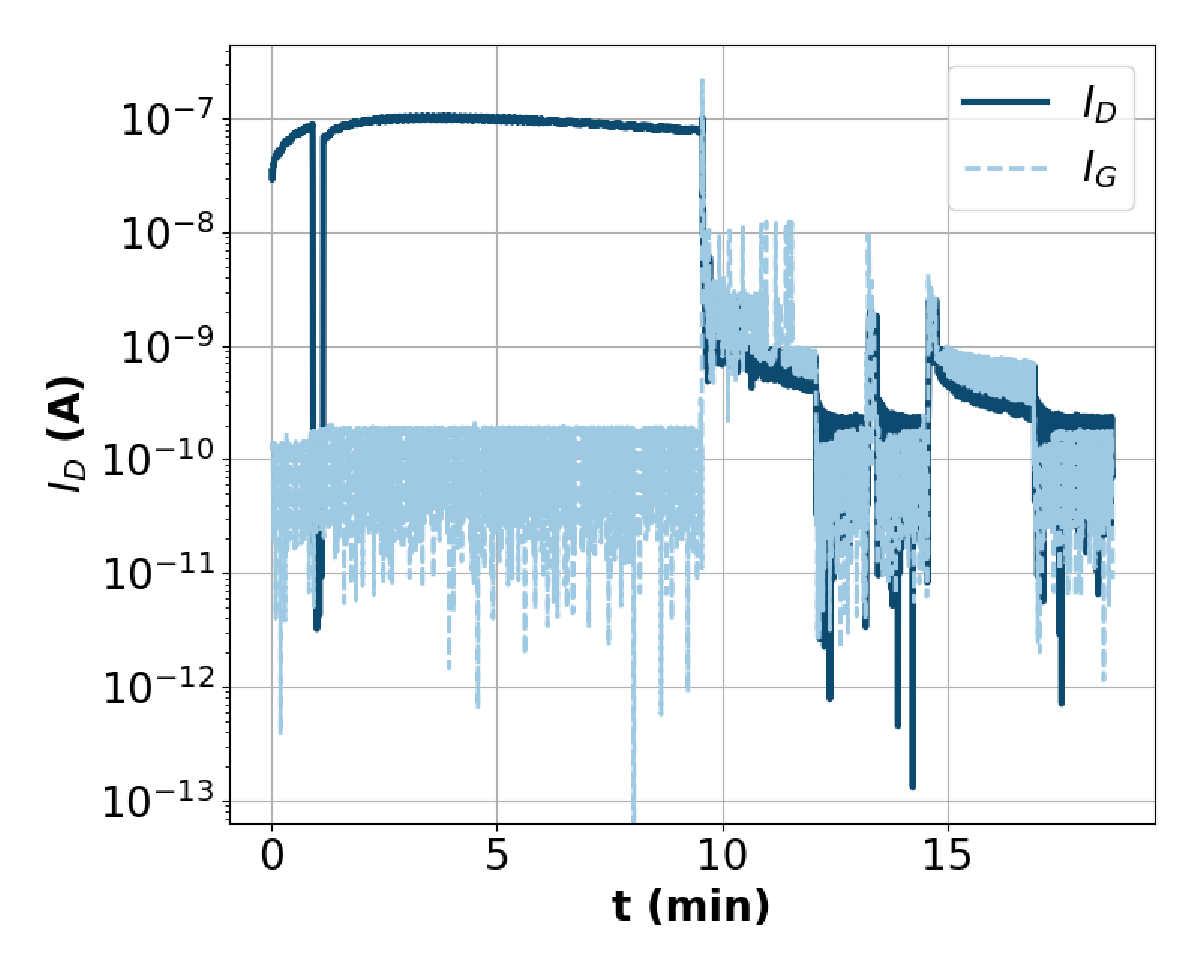
\includegraphics[width=7cm]{Images/pdf/elec-dedop1.pdf} }}
    \subfloat[]{{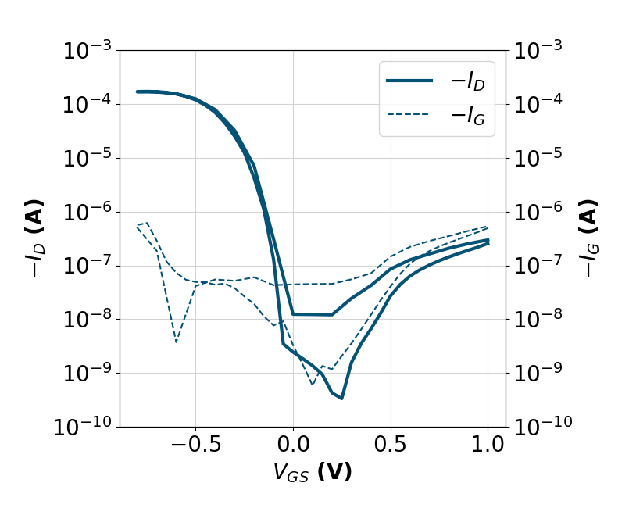
\includegraphics[width=7cm]{Images/pdf/Undoped_AgAgCl.pdf}}}
    %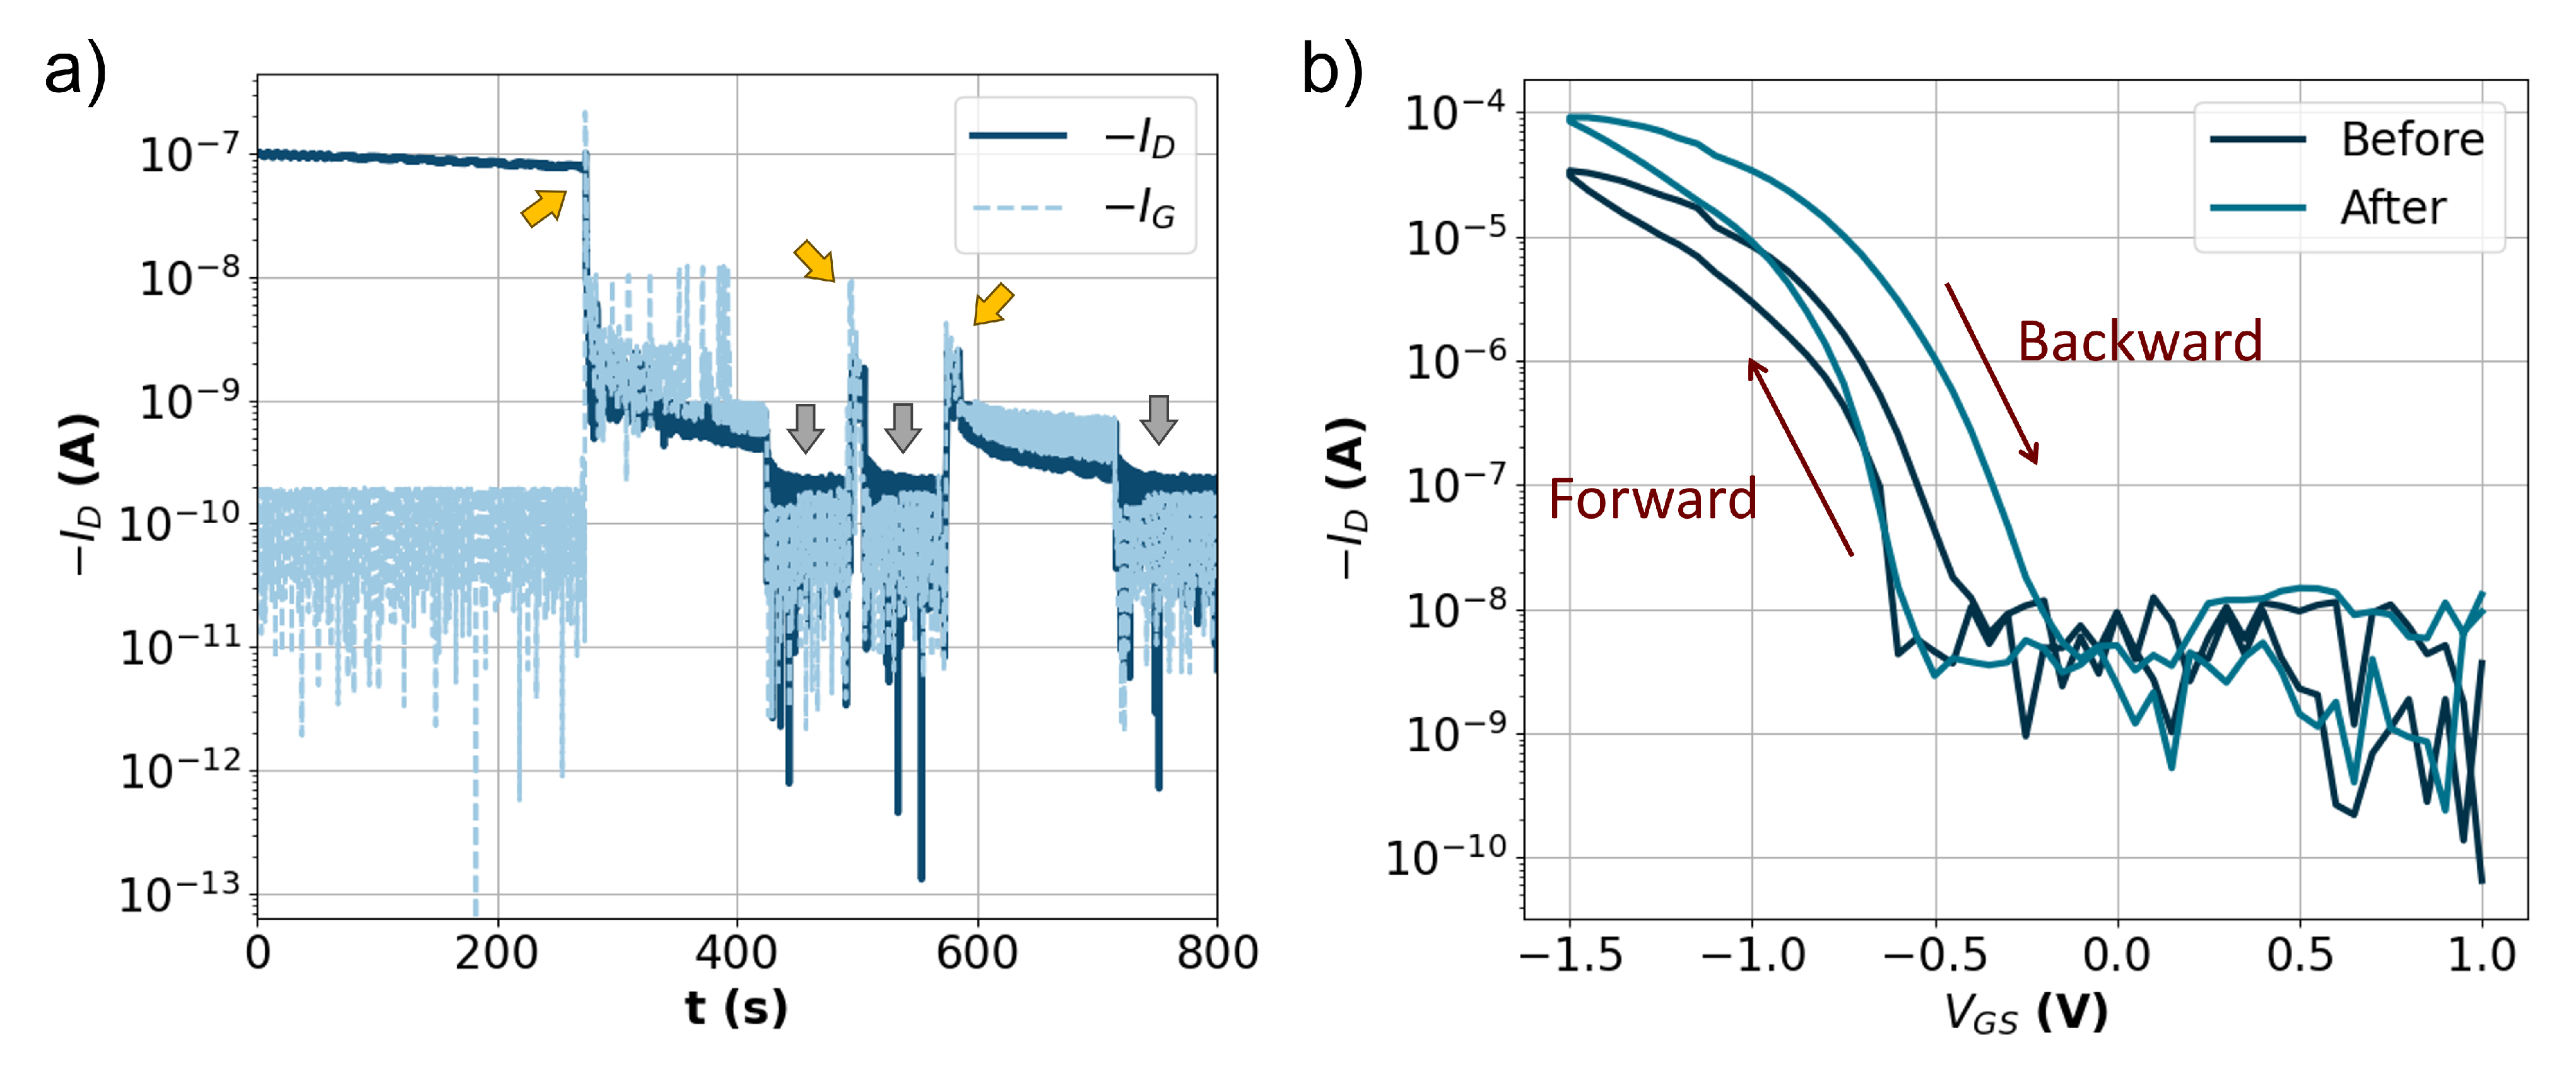
\includegraphics[width=\textwidth]{Images/pdf/de-doping.pdf}
    \caption[Electrochemical de-doping of oxidized p(g3T2-T) OECT]{a) De-doping p(g3T2-T) using a gate biased of +1V, gold arrows indicate gate connection, while grey arrows indicate when gate was disconnected. b) Transfer characteristics of device using Ag/AgCl under ambient conditions.}
    \label{fig:revox2}
\end{figure}

The subsequent experiment involved exposing the sample to ambient conditions, using the same device that underwent electrochemical de-doping. Unfortunately, it experienced degradation between measurements. Subsequently, transfer characteristics of another device from the same sample were measured using a Ag/AgCl pellet, as depicted in Figure \ref{fig:revox2}b. This measurement revealed a negative threshold voltage of -0.14 V, suggesting that drop-casted SSE, which will be further analyzed in the next section using the p(g3T2-T) gate, may be protecting p(g3T2-T) channel from spontaneous oxidation.
%, but still some interactions due to the redox peaks. (may need measurements outside for this one)

Figure \ref{fig:DropAgCl}a shows an increase in gate current from above +0.5 V and below -0.6 V, which is consistent with the increased leakage current in our device, and increase in drain current due to electrochemical doping of the channel. It is important to clarify that the redox peaks extracted from these measurements do not exclusively represent reduction and oxidation potentials between the working electrode (Ag/AgCl) and electrolyte. This is because the counter electrode and reference electrode are shorted and connected to the channel, which should be significantly large to minimize its effects on the electrolyte. Instead, these peaks represent crucial operation points for our OECT, where electron transfer is more pronounced. 

For instance, the oxidation peak may signify both the oxidation of the gate and the reduction of the channel, and the same applies to the reduction peaks. This approach will also be used and examined in the next section.

%D5
\begin{figure}[ht]
    \centering 
    %\sidesubfloat[]{{\hspace{-2em}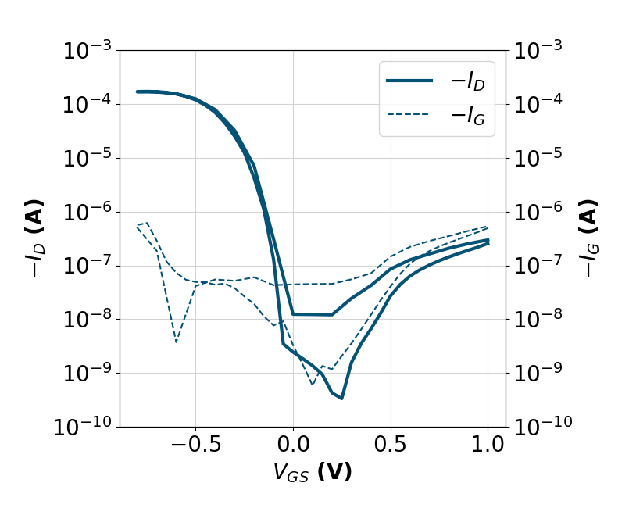
\includegraphics[width=7.5cm]{Images/pdf/Undoped_AgAgCl.pdf} }}
    %\qquad
    \sidesubfloat[]{{\hspace{-2.2em}
    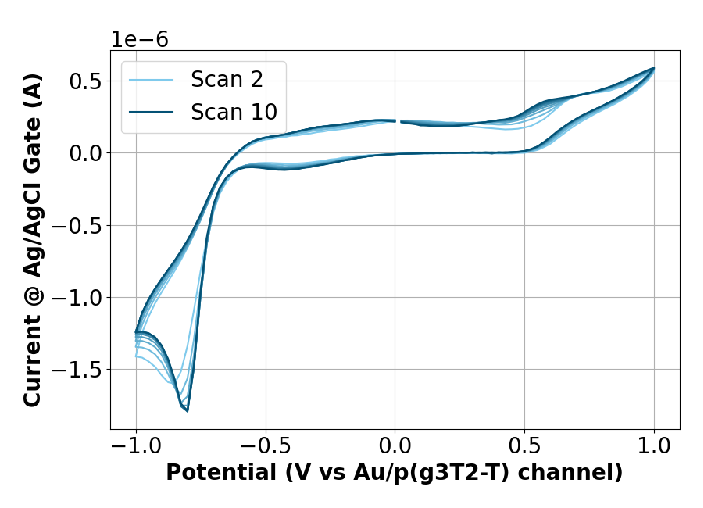
\includegraphics[width=7cm]{Images/pdf/CV_drop_AgClWE.pdf} }}
    \sidesubfloat[]{{\hspace{-2em} 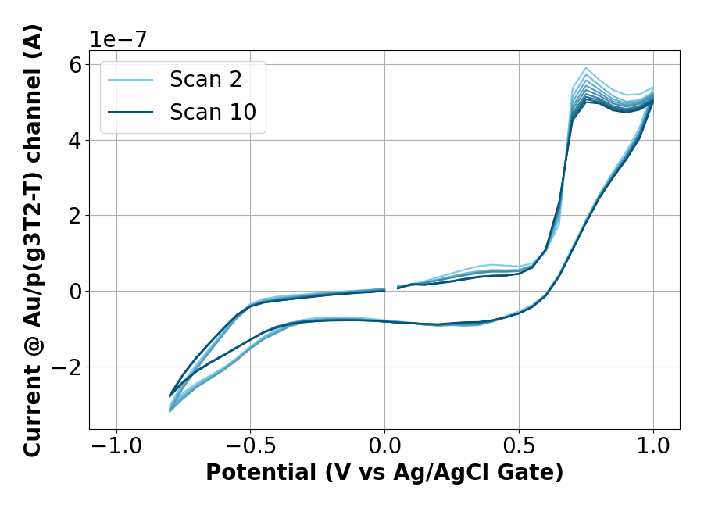
\includegraphics[width=7cm]{Images/pdf/CV_drop_AgClRECE.pdf} }}
    \caption[Transfer characteristics and cyclic voltammograms of device using Ag/AgCl gate under ambient conditions]{a) Transfer characteristics of device using Ag/AgCl gate under ambient conditions, and cyclic voltammograms using Ag/AgCl as b) working electrode and as c) counter electrode shorted with reference electrode.}
    \label{fig:DropAgCl}
\end{figure}

Meanwhile, measurements performed and represented in Figure \ref{fig:DropAgCl}b, where Ag/AgCl is now our counter electrode and it is significantly larger than our working electrode (Au/p(g3T2-T) channel), %, but also a reference electrode, which still will not give us a correct measurement of redox potential between the electrodes, but
can be correlated with the studies performed by Hidalgo Castillo et al. \cite{hidalgocastilloSimultaneousPerformanceStability2022a}, they reported a reduction potential at -0.4 V vs Ag/AgCl attributed to the interactions with molecular oxygen. Therefore, starting from at this operation point, ORR takes place, and as seen in Subsection \ref{subsec:sidereac}, there is high probabilities of forming hydrogen peroxide leading to degradation, the latter was evident in both devices tested in this subsection.

Although, we are biasing our channel to values that exceed operational range, this will hold true when using our OMIEC gate. %Therefore, it is a point to take into consideration.

%\subsubsection{By Heating}

%**\textit{I was thinking of initiating this subsection with the shift of threshold voltage with temperature but not sure anymore. I have a similar sentence as the following in the photolithography SSE OECT, but I am thinking on moving it here because it is a way to revert the oxidation of p(g3T2-T), and I use it for the photo and printed SSE, I do not use the electrochemical dedoping in both}**

%Before the application of adhesion promoter to enhance adhesion between SSE and patterned polymer channel and gate. An ethanol rinsing followed by the high-temperature baking step is done, as explained in Subsection \ref{subsec:solidOECT}. The following reaction: \\

%C_{2}H_{6}O_{(l, ethanol)} + 2O_{2}_{(g)} \arrow 2 CO_{2}_{(g)} + 3H_{2}O_{(g)}
%\hspace{3cm} \ce{ C2H6O_(l) + 2O2_(g) -> 2CO2_(g) + 3H2O_(l)} \\

%describes the interaction between ethanol and oxygen, and together with the temperature step, it was perceived that they helped to counteract the oxidation of the polymer.
%What temperature, time?

%**\textit{I need to check if I have measurements more than pictures, I base this miniconclusion in reflection hue and transfer curves achieved}**

%\newpage
\section{Fabrication of Side-Gate Organic Electrochemical Transistors}
%\subsection{Undoped-p(g3T2-T)}

In the previous section, an investigation into the doping of the p(g3T2-T) channel was conducted, and attention was given to the issues of unwanted oxidation, dopant stability and ORR. With these considerations in mind, the focus now shifts to the fabrication of solid-OECTs. 

First, the fabrication of undoped p(g3T2-T) devices will be addressed by simply drop-casting SSE on top of the fourteen pattern devices. With these initial findings, this approach will be refined by structuring the electrolyte by i) photolithography \cite{weissbachPhotopatternableSolidElectrolyte2022} and ii) inkjet printing. 

Following the comparison of these three device architectures, doped solid-OECTs will be fabricated, and their threshold voltage shifts upon doping will be evaluated. %Additionally, the usefulness of the doping for solid OECTs will be assesses.

%The fabrication of OECTs using a solid-state electrolyte at IAPP %, to enable IC and thermodynamics studies, 
%was established in reference  \cite{weissbachPhotopatternableSolidElectrolyte2022}, the electrolyte that formed PNIPAm upon UV light exposure is more precisely considered as a rigid gel.
%consists of monomer units, including NIPAm and HHPA, as outlined in Chapter \ref{cha:2} Section \ref{tab:sse}. such as N-isopropylacrylamide (NIPAm) and 2-hydroxy4’-(2-hydroxyethoxy)-2-methylpropiophenone (HHPAA) upon exposure to UV light, these monomers cross-link, forming the polymer poly(N-isopropylacrylamide) (PNIPAm), which is more precisely considered as a rigid gel. 
%Two types of OECTs were tested under a $N_{2}$ environment and later exposed to ambient conditions. In one type, SSE couples all fourteen devices in the sample, while in the other type, each device possesses a microstructure SSE. The latter strategy enhances the performance of OECTs by minimizing leakage current and avoiding device crosstalk. This can be achieved through a photolithography process, as outlined in reference \cite{weissbachPhotopatternableSolidElectrolyte2022}, or by inkjet printing, as implemented by team members. Both methods were employed under normal cleanroom conditions to determine which  approach minimizes oxidation or allows for the reverse oxidation of p(g3T2-T) within the process. 
%In this subsection, a total of three samples will be analyzed, it is expected to have low degree of oxidation in all devices.
%Finally, one of each type of sample was exposed to air to understand ORR effects. It is expected to see oxidation in all devices.

\subsection{Undoped Drop-casted SSE}%Solid-State Electrolyte}
At this point, the patterning process had improved its yield, with twelve out of the fourteen devices being successfully patterned, although there were some variations in thickness, as evidenced by the reflection hue of the micrographs. Among these devices, only seven remained operational.
 %by improving homogeneity of dynamic spin-coating, say patterning number, %before and after exposure could be appendix, right now I will place it before

Electrochemical de-doping of one device in the sample was carried out before exposure. Transfer curves using the p(g3T2-T) gate showed a negative turn-on voltage (Figure \ref{fig:revox2}). Additionally, a transfer curve was measured after exposure to UV light. The monomer units in the SSE (NIPAm and HHPA) cross-link upon exposure forming the polymer poly(N-isopropylacrylamide) (PNIPAm), then an increase in current upon crosslinking is observed.

\begin{figure}[ht]
    \centering
    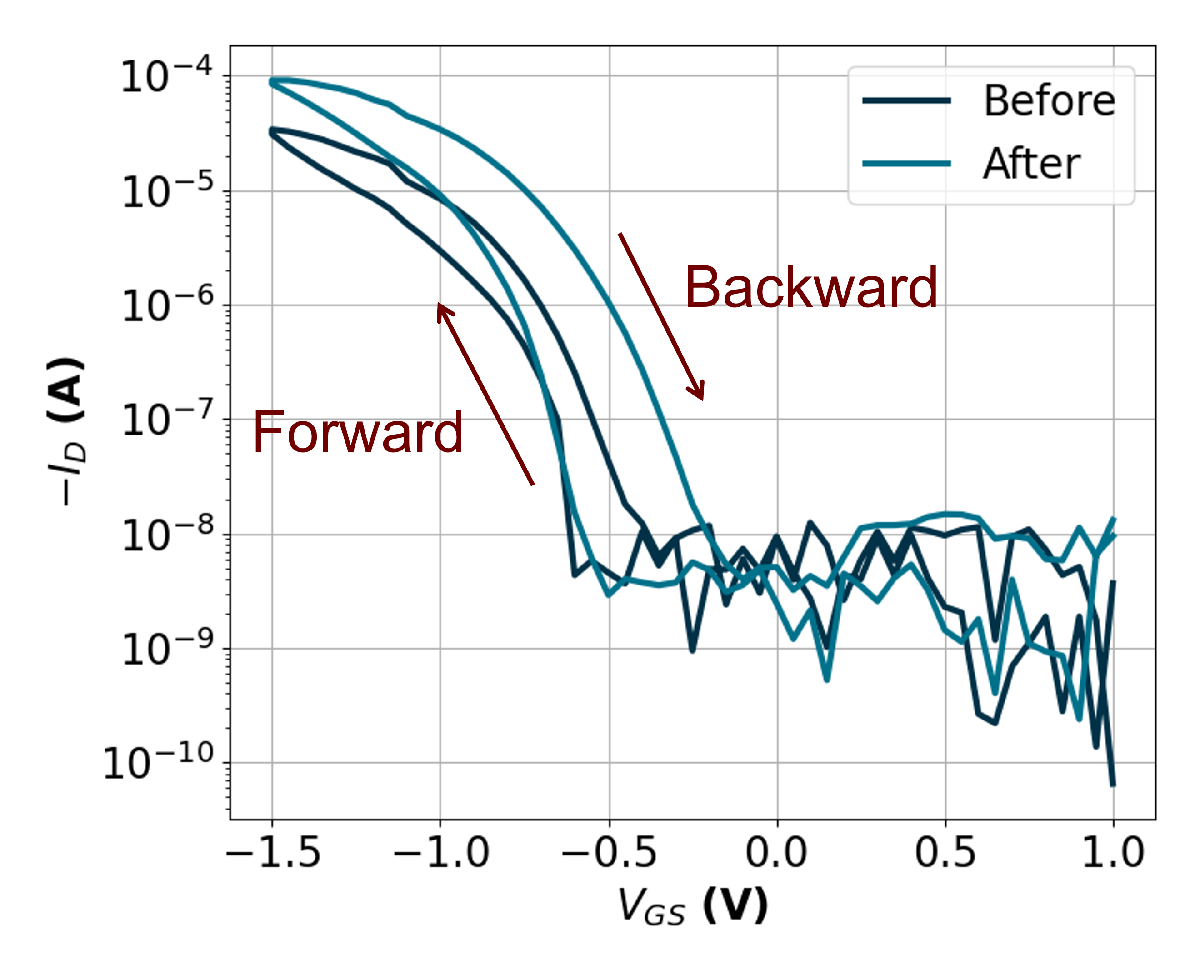
\includegraphics[width=7cm]{Images/pdf/transfer_de-dop_exp.pdf}
    %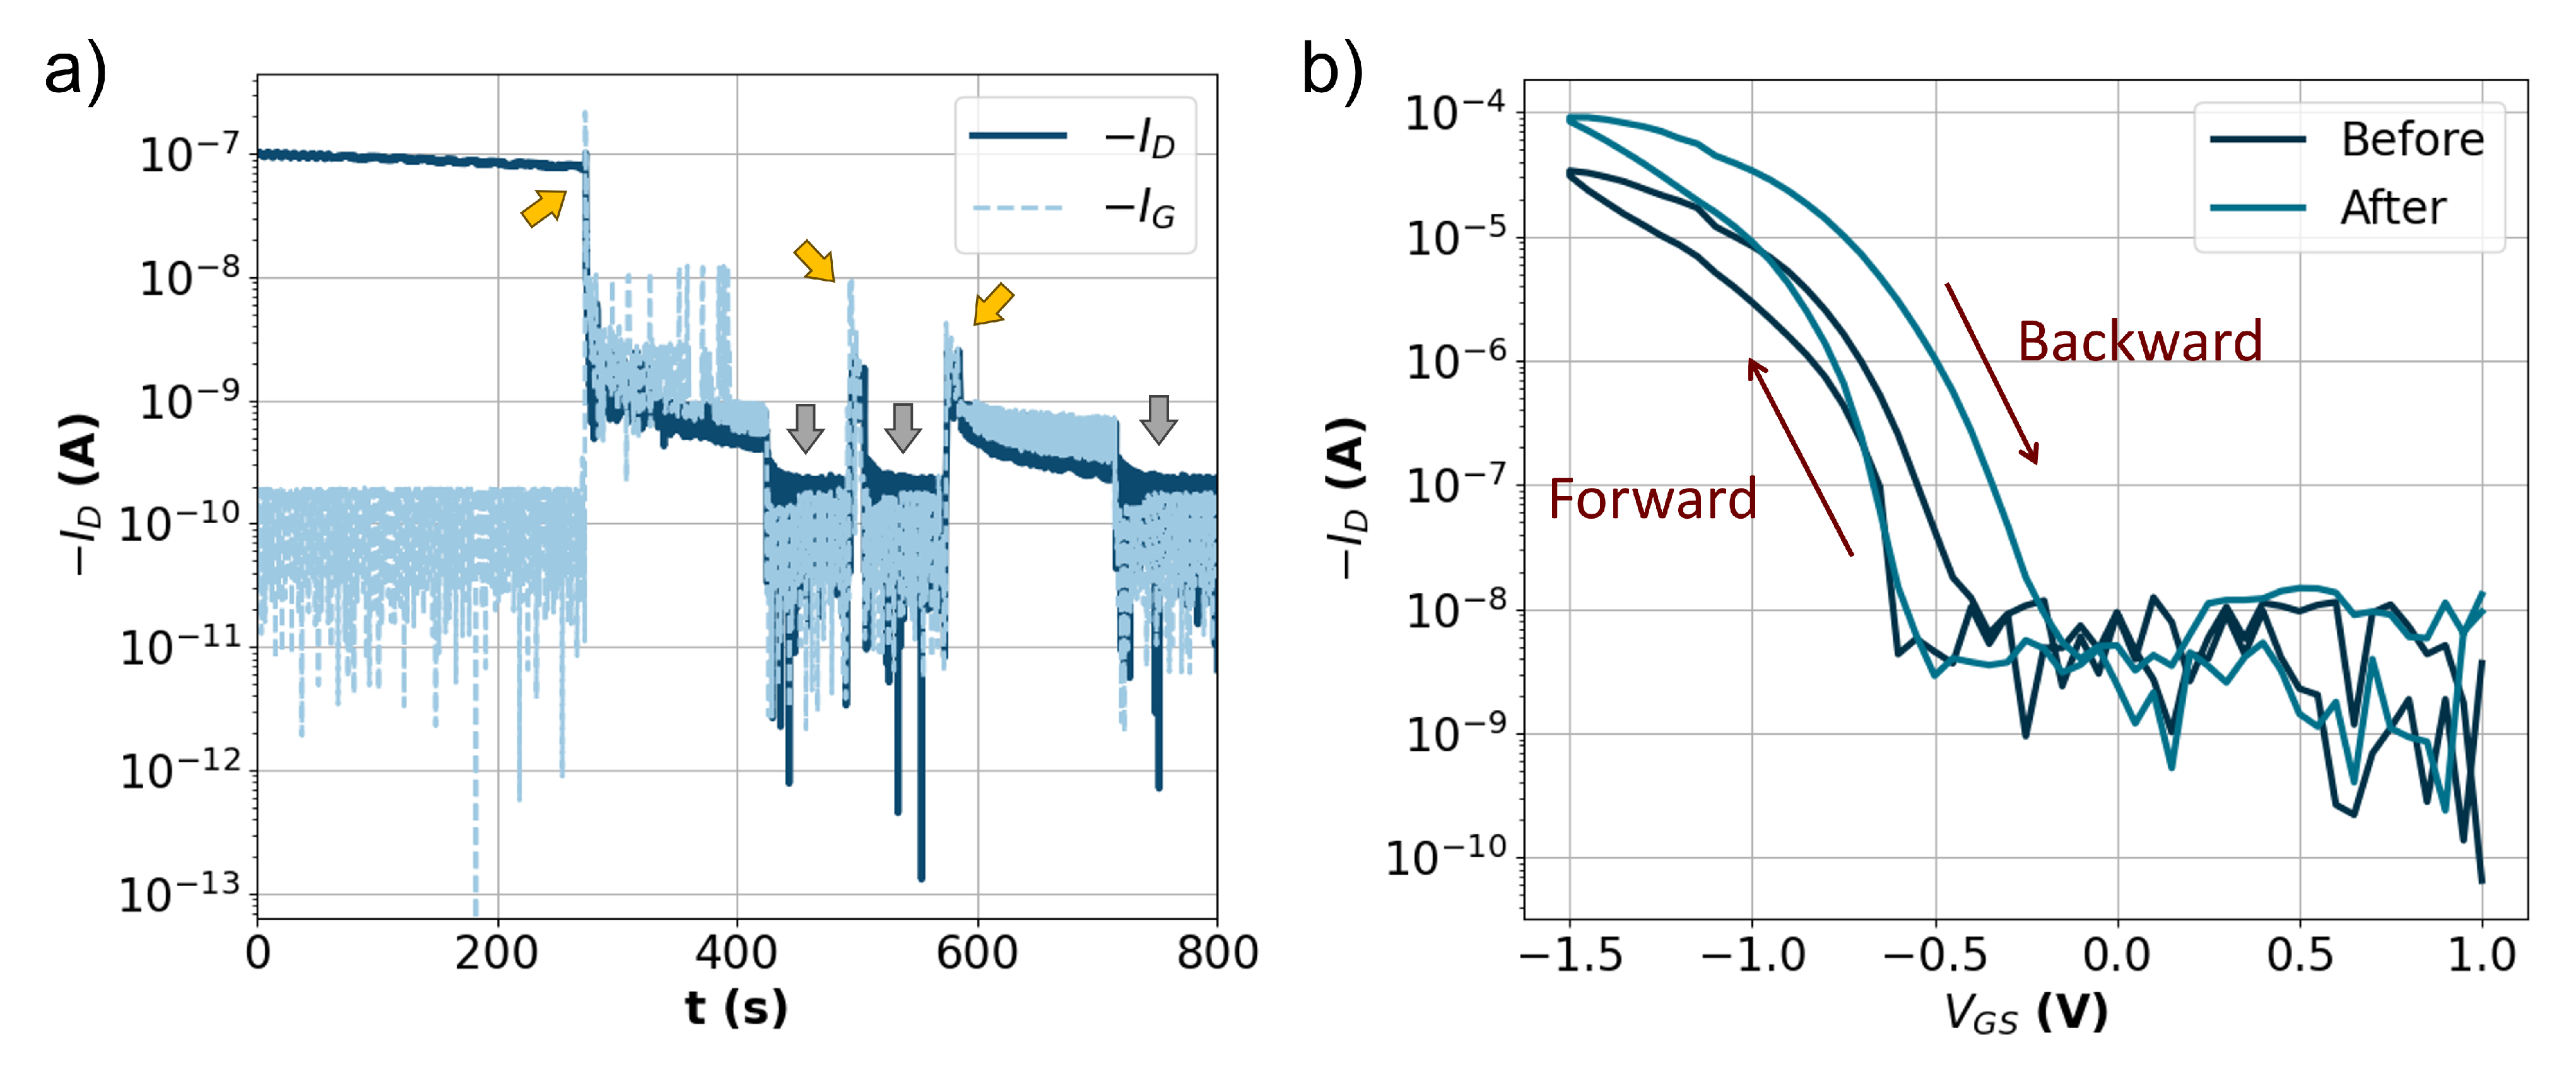
\includegraphics[width=\textwidth]{Images/pdf/de-doping.pdf}
    \caption[Transfer characteristics of side-gate OECT with pristine p(g3T2-T)]{Transfer characteristic before and after exposure to UV light at $V_{DS}$ of -0.1 V using p(g3T2-T) gate coupled with SSE precursor.}
    \label{fig:revox2}
\end{figure}
%%%

Moreover, it was perceived that using the OMIEC gate instead of the Ag/AgCl pellet affects our ``gating efficiency'', as expected. Weissbach et al.  \cite{weissbachUnravelingElectrochemicalElectrode2023} demonstrated the Electrochemical Electrode Coupling (ECC) between channel and its electrode has a more pronounce effect on device operation when micro-integrated polarizable gates (OMIECs) are used. This coupling can result in saturation loss %(as seen in Figure \ref{fig:revox2}b)
and threshold voltage roll-of when increasing $V_{DS}$, which was observed during measurements. Therefore, moving forward, $V_{DS}$ will be fixed at -0.1 V.

Measurements of channel conductivity of the other devices indicated an impact of this process to neighboring devices (a total of 5) as most of them had very low conductivity, in the order of nS. One exception exhibited a conductivity in the order of $\mu$S and a threshold voltage of 0.0 V. Moreover, attempts to perform irreversible electrochemical de-doping on this device after cross-linking of monomer units were unsuccessful. It appeared that the formation of PNIPAm prevented irreversible dedoping. This outcome is crucial for the fabrication of doped-devices and will be discussed further in Section \ref{subsec:dopedOECTs}.

Subsequently, other four devices from the sample were measured under the conditions detailed in Section \ref{subsec:solidOECT}. A representative device can be seen in Figure \ref{fig:dropcast}a, note that this sample was used for reverse oxidation experiments, the reflection hue changed from brownish to bluish color after lowering its conductivity. SSE precursor was blew off and a new drop was deposited for the solid-OECT. 

%D1
\begin{figure}[ht]
    \centering
    \subfloat[]{{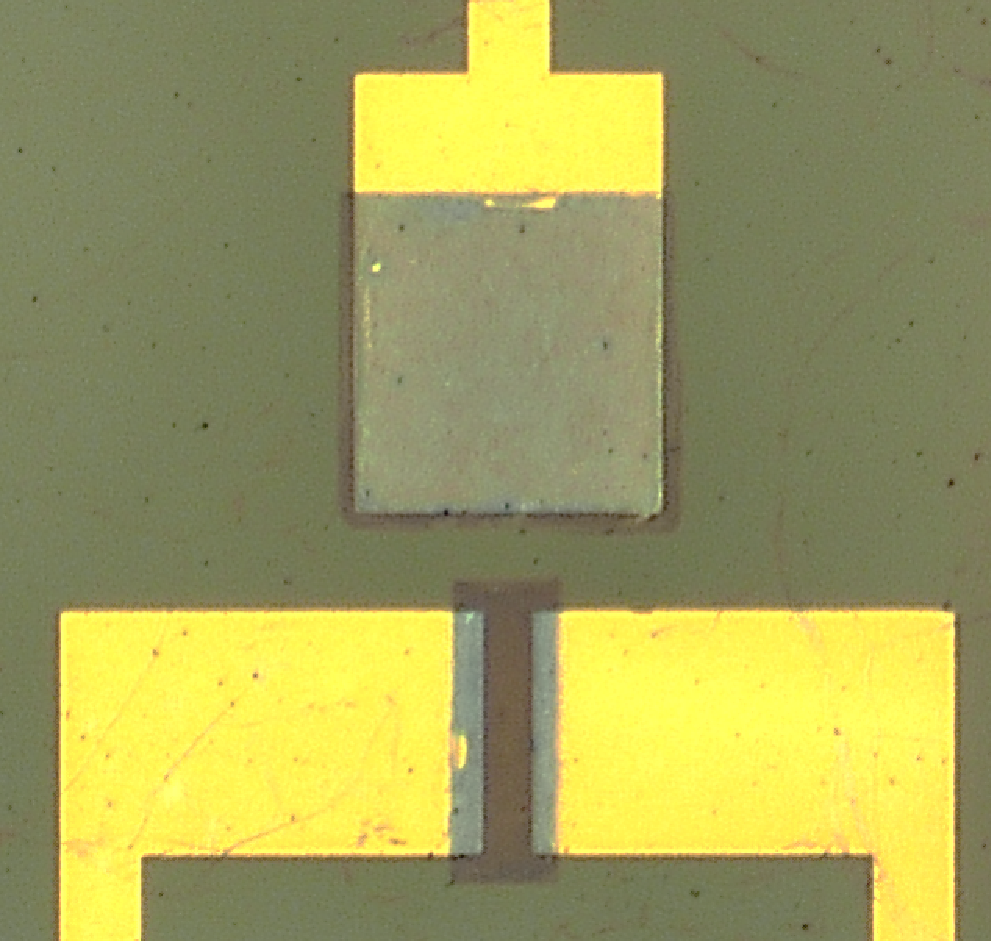
\includegraphics[width=3.5cm]{Images/pdf/und_drop.pdf} }}
	\hspace{3em}    
    \subfloat[]{{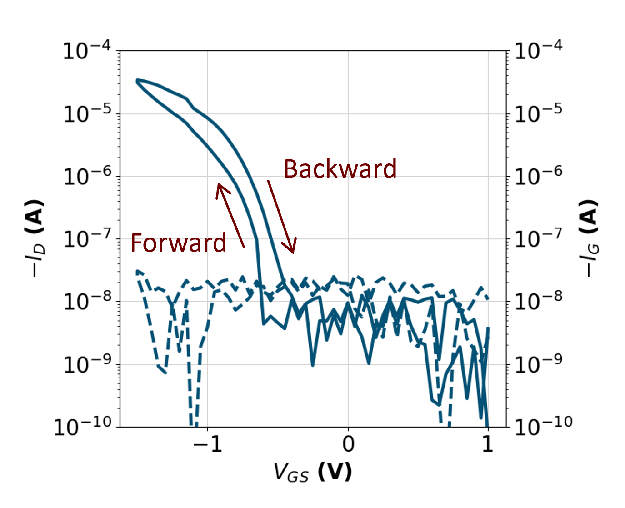
\includegraphics[width=7cm]{Images/pdf/transfer_de-dop.pdf} }}
    \qquad
    \subfloat[]{{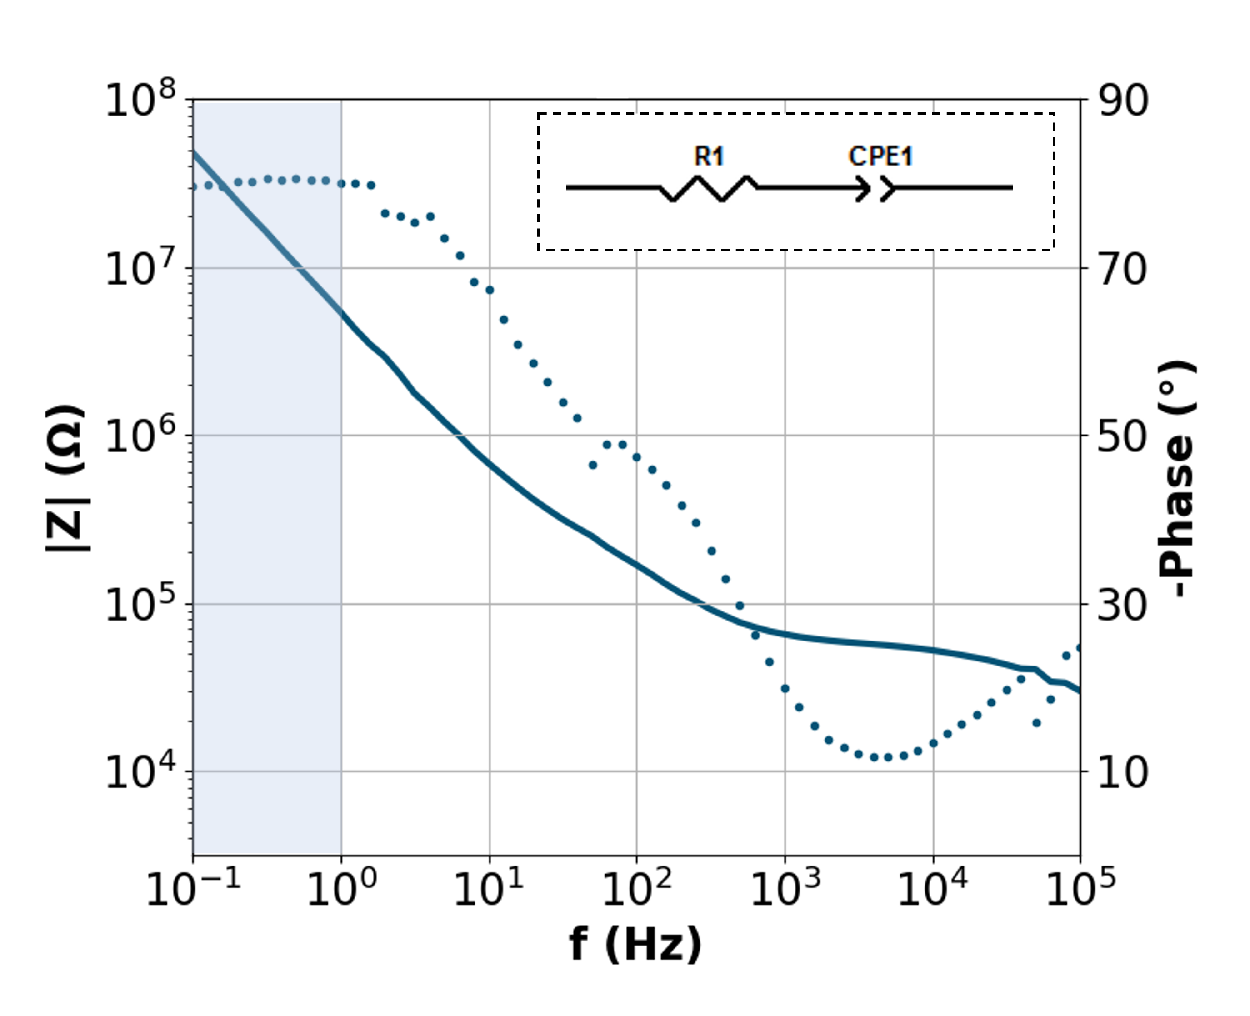
\includegraphics[width=7cm]{Images/pdf/EIS_drop.pdf} }}
    \subfloat[]{{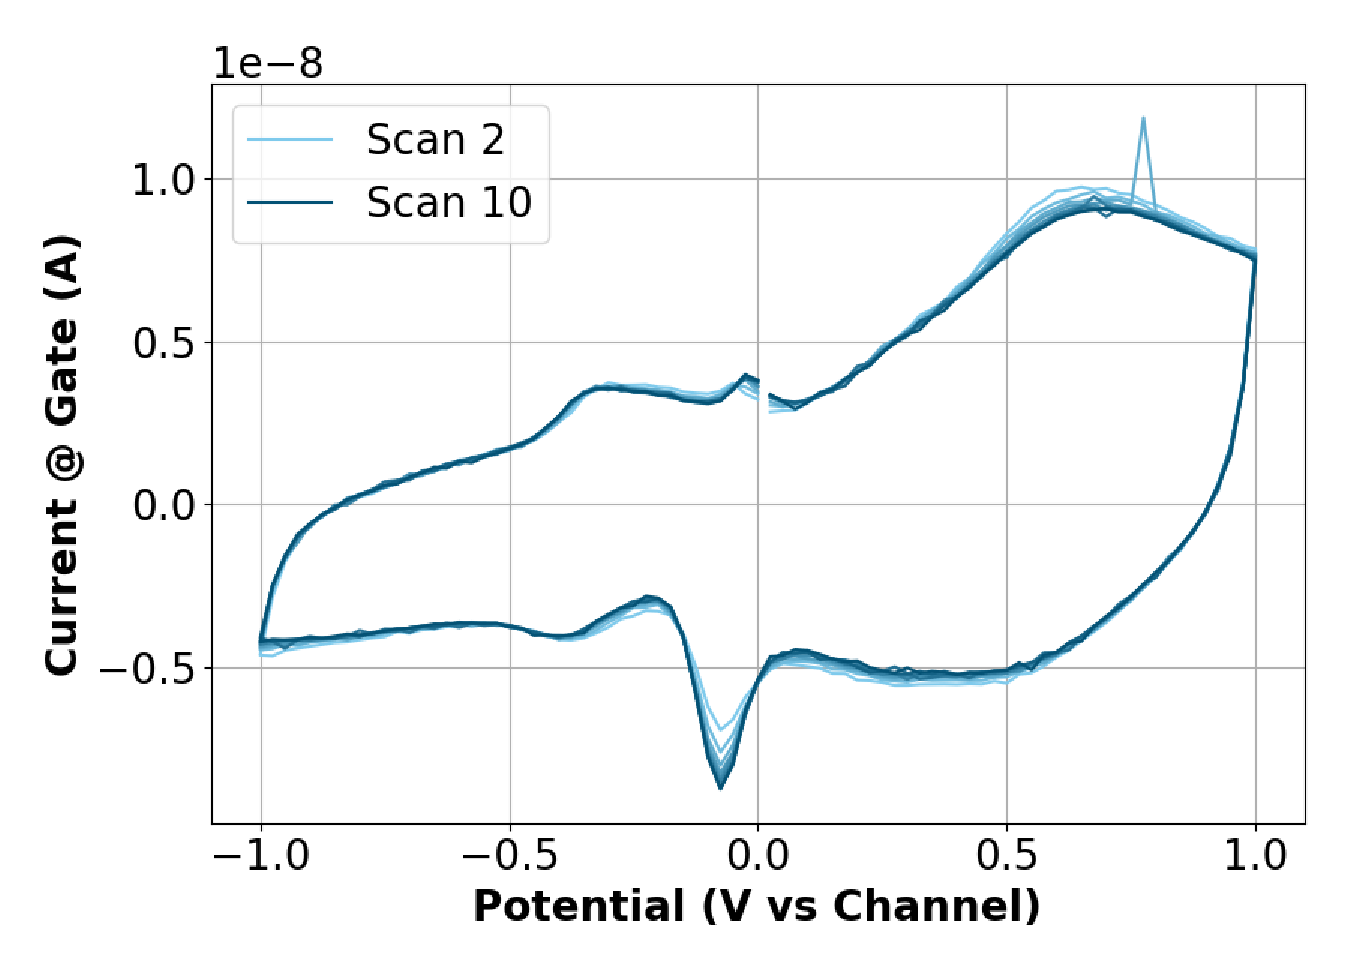
\includegraphics[width=7cm]{Images/pdf/CV_drop.pdf} }}
    \caption[Performance of solid-OECT with drop-casted SSE]{a) Micrograph of patterned device before application of SSE, b) transfer characteristics at $V_{DS}$ of -0.1 V. And representative c) Bode plot obtained by EIS and d) cyclic voltammograms.}
    \label{fig:dropcast}
\end{figure}

Transfer characteristics exhibited a |g$_{m,max}$| value of 79 $\mu$S. Threshold voltages were calculated for forward and backward scans, that led to values of 0.09 V and -0.06 V, respectively, exhibiting a small hysteresis. Further analysis on hysteresis is considered beyond the scope of this work. 

Using EIS measurements and fitting into the equivalent circuit model (inset image at Figure \ref{fig:dropcast}c) lead to $C_{channel}$ of 34.0 nF and C* calculations yield to 36.5 Fcm$^{-3}$, much lower than the 211 $\pm$ 18 Fcm$^{-3}$ \cite{moserEthyleneGlycolBasedSide2020} or 144 Fcm$^{-3}$ \cite{hidalgocastilloSimultaneousPerformanceStability2022a} reported in the literature. 
%It is important to clarify that the redox peaks extracted from these measurements do not exclusively represent reduction and oxidation potentials between the working electrode (Au/p(g3T2-T)) and electrolyte. This is because the counter electrode and reference electrode are shorted and connected to the channel, which should be significantly large to minimize its effects on the electrolyte. Instead, these peaks represent crucial operation points for our OECT, where electron transfer is more pronounced.
%For instance, the oxidation peak may signify both the oxidation of the gate and the reduction of the channel, and the same applies to the reduction peaks. Furthermore, these peaks correlated with observed behavior in transfer characteristics: Appendix \ref{app:CV} shows how a device with some fabrication defects showing a large hysteresis on the transfer characteristics, redox potentials in this device also exhibit the same behavior. 

Furthermore, cyclic voltammograms exhibit major oxidation and reduction peaks of +0.65 V and -0.08 V, respectively, with a smaller but significant reduction peaks at -0.32 V and oxidation peak at -0.01 V. Redox potentials close to the turn-on voltage values in this device can be correlated with the low hysteresis observed in transfer characteristics: Appendix \ref{app:CV} shows how a device with some fabrication defects showing a large hysteresis on the transfer characteristics. 

The major reduction peak, on the other hand, occurs when device is at the OFF state, no major changes are perceived in $I_{D}$, but a big decrease in $I_{G}$. Additionally, from our observations from Subsection \ref{subsec:revox}, the presence of redox potentials outside the turn-on voltages observed in both the channel and gate may indicate the occurrence of ORR in our device due to the remaining degree of oxidation in both our channel and gate. Further experiments are needed to confirm this hypothesis. For instance, cyclic voltammetry measurements under controlled oxygen-saturated environments should be conducted using an ideal electrical configuration, including a large counter electrode and a separate reference electrode.
%It is still unclear what factors influence the positions of the redox peaks, as an hypothesis, as reviewed in Subsection \ref{subsec:revox}, redox potential outside the operational points of our OECTs, may be indications of ORR happening in the channel and gate, indicating some degree of oxidation in between our patterned structures. %what determines the higher peak potential.
%Particularly for this case, peaks occurring away from the vicinity of 0 V could indicate interaction with oxygen or the presence of defects in our devices. 

A statistical analysis on the four devices are shown in Table \ref{tab:dropfom}. Most importantly, negative threshold voltages were calculated. Additionally, all exhibited the same prominent oxidation peak (0.68 $\pm$ 0.02 V), but only peaks close to the turn-on voltages are reported. %Very low values of capacitance were obtained, which may indicate the presence of defects (i.e. remnants of photoresist). %Additionally, the geometry of the devices could contribute to these low capacitance values
%The shadowed area of the Bode plot illustrated in Figure \ref{fig:dropcast}c (low frequencies) was used to calculate the channel capacitance and volumetric capacitance, as shown in Table \ref{tab:dropfom}. 


%%U3 before D7
\begin{table}[ht]
\centering
\caption{Parameters extracted from the characterization of drop-casted SSE OECTs}
\begin{tabular}{l|c||l|c}
Parameters & Value & Parameters & Value \\\hline \hline
V$_{Th,forward}$ [V] & -0.30 $\pm$ 0.13 & V$_{Th,backward}$ [V] & -0.17 $\pm$ 0.08\\
& & &\\[-1em]
C$_{channel}$ [nF] & 40.9 $\pm$ 12.2 & C* [Fcm$^{-3}$] &  43.9 $\pm$ 13.1 \\
%C$_{channel}$ [nF] & 36 $\pm$ 10 & C* [Fcm$^{-3}$] & 38 $\pm$ 10 \\
& & &\\[-1em]
V$_{ox}$ [V] & -0.33 $\pm$ 0.05 & V$_{red}$ [V] & -0.42 $\pm$ 0.19 %\\
%& & &\\[-1em]
%|g$_{m,max}$| [$\mu$S] & 0.07 $\pm$ 0.07 &  &
\\\hline
\end{tabular}
\label{tab:dropfom}
\end{table}

\subsection{Undoped Photopatterned SSE} %Solid-State Electrolyte}
This trial resulted in ten out of fourteen operational devices. %A micrograph of a representative device can be seen in Figure \ref{fig:photoSSE}a. 
However, certain devices exhibited unusual behavior due to defects, or some SSE partially removed from the device. These devices were excluded from the analysis, leaving us with a total of seven devices.

The microstructuring of SSE on top of the OMIEC channel and gate required the use of an adhesion promoter, which differs from the drop-casted SSE. In this particular case, the removal of non-crosslinked SSE precursor was achieved using a $N_{2}$ gun, using an adhesion promoter reduces the risk of removing crosslinked SSE. %Moreover, as explained before, it serves as a method to revert the oxidation of the p(g3T2-T) film.
Morever, the application of the adhesion promoter was followed by an ethanol rinsing and high-temperature baking steps at 100$^{\circ}$C, as explained in Subsection \ref{subsec:soect}. Both of these steps helped to reverse the oxidation of the polymer. Ethanol initiates a reaction with oxygen as described below: \\

%C_{2}H_{6}O_{(l, ethanol)} + 2O_{2}_{(g)} \arrow 2 CO_{2}_{(g)} + 3H_{2}O_{(g)}
\hspace{2.5cm} \ce{\centering C2H6O_{(l)} + 2O2_{(g)} -> 2CO2_{(g)} + 3H2O_{(l)}} \\ 

The baking step evaporates the water content in the polymer formed by the reaction. Therefore, electrochemical de-doping before SSE patterning was not necessary. This approach will be used for the following samples.

A representative device can be seen in Figure \ref{fig:photoSSE}a, device exhibit signs of oxidation indicated by the brownish hue. Micrograph was taken before the application of the adhesion promoter. 

Transfer characteristics, depicted in Figure \ref{fig:photoSSE}b, exhibited a |g$_{m,max}$| value of 139 $\mu$S. Threshold voltages of -0.10 V and -0.18 V for forward and backward scans, respectively, with a small hysteresis. 

From the EIS results shown in Figure \ref{fig:photoSSE}c, a $C_{channel}$ of 34.5 nF and C* of 37.0 Fcm$^{-3}$ were calculated. Cyclic voltammograms gave prominent oxidation and reduction peaks of +0.03 V and -0.20 V, respectively, closer to turn-on voltages, as seen in Figure \ref{fig:photoSSE}d, with smaller, but significant oxidation peaks at -0.32 V and +0.57 V.
%%U3 before D5

\begin{figure}[!htb]
    \centering
    \subfloat[]{{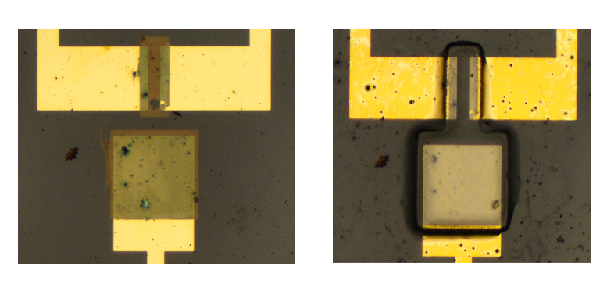
\includegraphics[width=7cm]{Images/pdf/und_photo.pdf} }}
    %\hspace{2em}
    \subfloat[]{{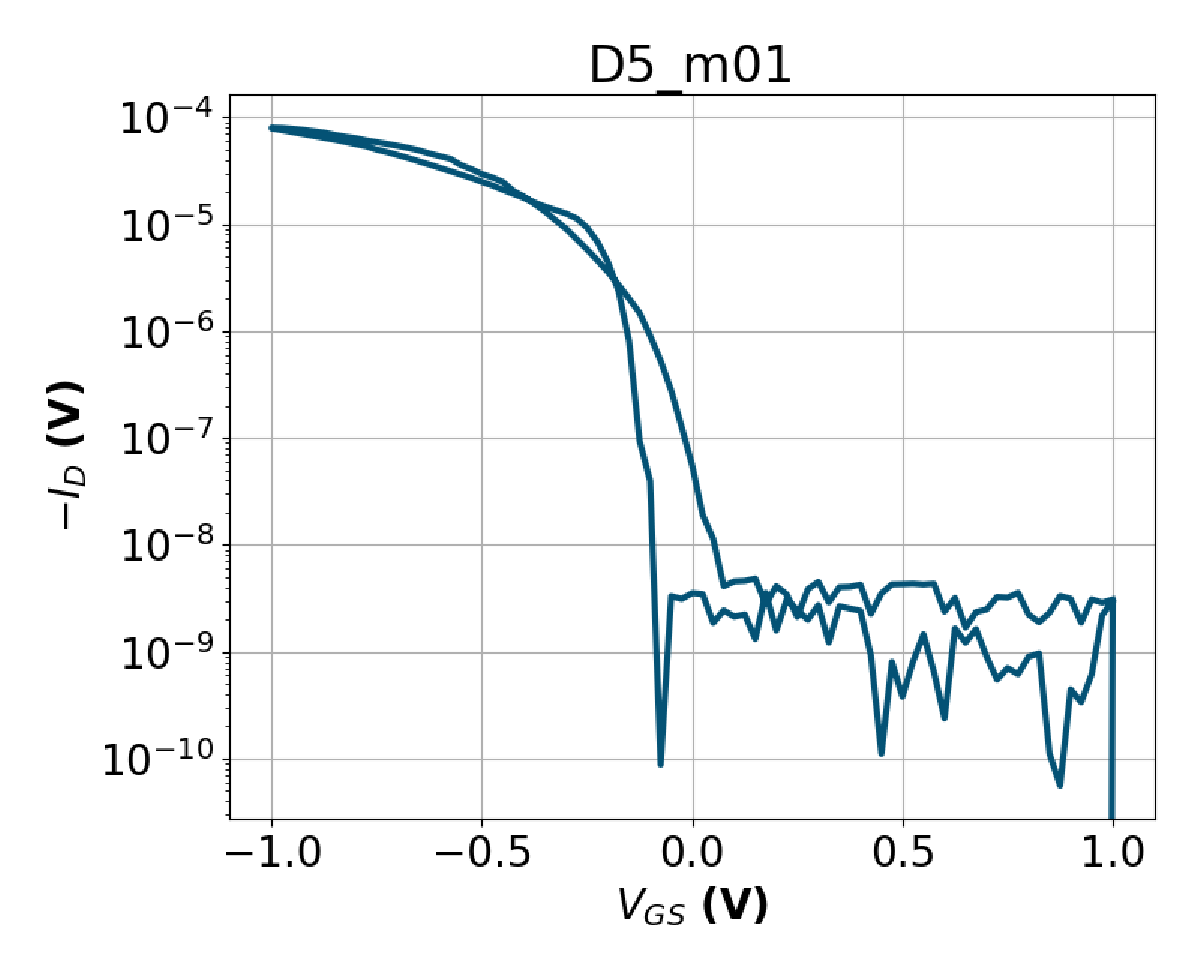
\includegraphics[width=7cm]{Images/pdf/transfer_photo.pdf} }}
    \qquad
    \subfloat[]{{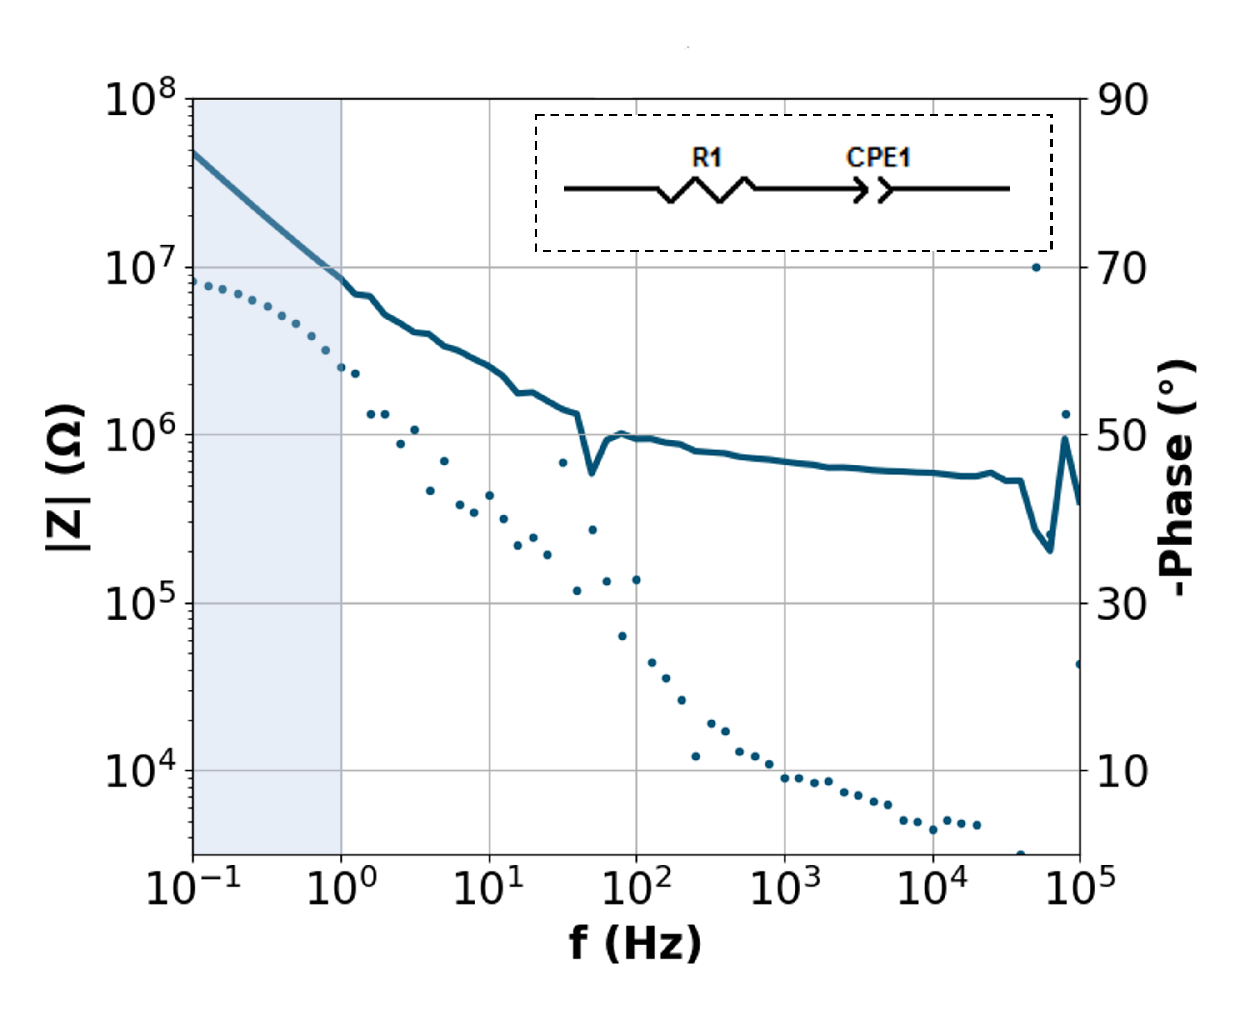
\includegraphics[width=7cm]{Images/pdf/EIS_photo.pdf} }}
    \subfloat[]{{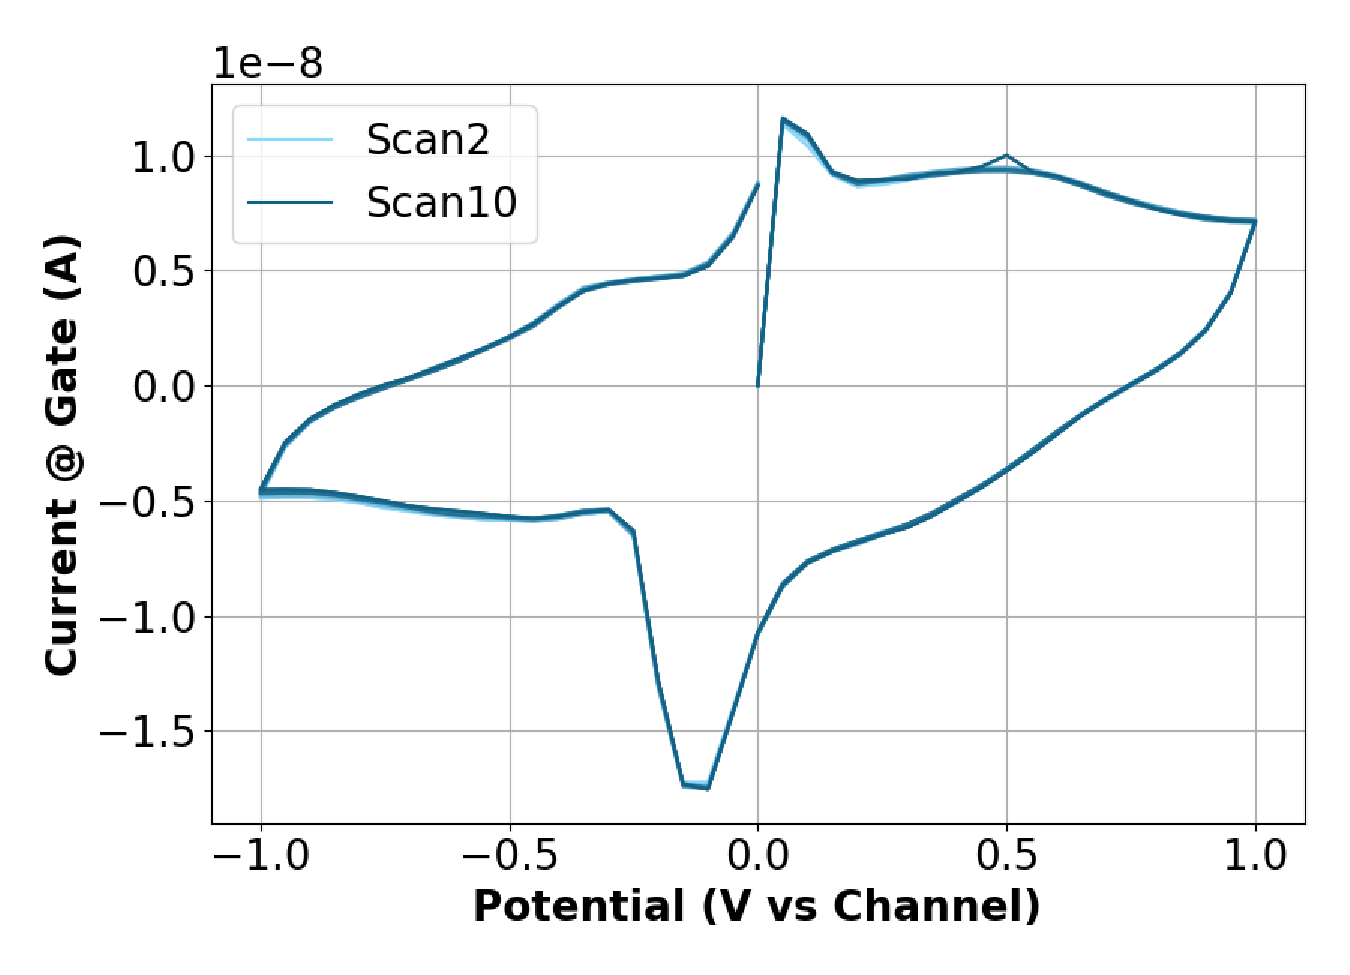
\includegraphics[width=7cm]{Images/pdf/CV_photo.pdf} }}
    \caption[Performance of solid-OECT with photolithographed SSE]{a) Micrograph of patterned device before and after application of SSE, b) transfer characteristics at $V_{DS}$ of -0.1 V. And representative c) Bode plot obtained by EIS and d) cyclic voltammograms.}
    \label{fig:photoSSE}
\end{figure}

A statistical analysis of all devices is shown in Table \ref{tab:photofom}. Importantly, negative threshold voltages were calculated, although not as negative as the electrochemical de-doping ones from previous subsection.

\begin{table}[ht]
\centering
\caption{Parameters extracted from the characterization of photopatterned SSE OECT under $N_{2}$ environment.}
\begin{tabular}{l|c||l|c}
Parameters & Value & Parameters & Value \\\hline \hline
V$_{Th,forward}$ [V] & -0.08 $\pm$ 0.05 & V$_{Th,backward}$ [V] & -0.09 $\pm$ 0.04\\
& & &\\[-1em]
C$_{channel}$ [nF] & 51.1 $\pm$ 17.7 & C* [Fcm$^{-3}$] & 54.9 $\pm$ 19.0 \\
%C$_{channel}$ [nF] & 58.7 $\pm$ 24.4 & C* [Fcm$^{-3}$] & 63.1 $\pm$ 26.2 \\
& & &\\[-1em]
V$_{ox}$ [V] & -0.01 $\pm$ 0.20 & V$_{red}$ [V] & -0.11 $\pm$ 0.09  \\
& & &\\[-1em]
|g$_{m,max}$| [$\mu$S] & 107 $\pm$ 162 &  &\\\hline
\end{tabular}
\label{tab:photofom}
\end{table}

Regarding cyclic voltammograms, only redox peaks close to turn-on voltages are reported, which were not necessarily the most prominent ones, unlike representative device. Another identified oxidation potential in all devices was 0.46 $\pm$ 0.09 V, which falls within the values identified in the previous device configuration (drop-casted SSE).

The channel and volumetric capacitance show a clear increase compared to drop-casted SSE, possibly due to persistent degree of oxidation of p(g3T2-T) that enhances channel conductivity. 

%, this may be due to the lack of device crosstalk
%However, CV graphs exhibit two different behaviors, with oxidation and reduction potentials falling into the ranges represented in Table \ref{tab:photofom}, suggesting that some oxidation is still perceived in most devices. %After the application of SSE precursor and exposure, the transfer curves (seen in Figure \ref{fig:photoSSE}b) indicate slight hysteresis, turn-on voltages close to zero, and slightly negative threshold voltages, as shown in Table \ref{tab:photofom}. These values are higher compared to the samples with drop-casted SSE. Cyclic voltammetry measurements gave oxidation and reduction peaks of -0.3 V and -0.1 V, with some smaller oxidation peaks at 0.6 V and -0.2 V. 

Upon exposure to ambient environment conditions, measurements revealed depletion-mode devices with a positive turn-on and threshold voltages, as depicted in transfer characteristics shown in Figure \ref{fig:photoSSEair}a. This suggests that, unlike drop-casted SSE, photopatterned SSE does not provide sufficient ``shielding'' to prevent oxidation of p(g3T2-T). 

%%U3
\begin{figure}[ht]
    \centering
    %\subfloat[]{{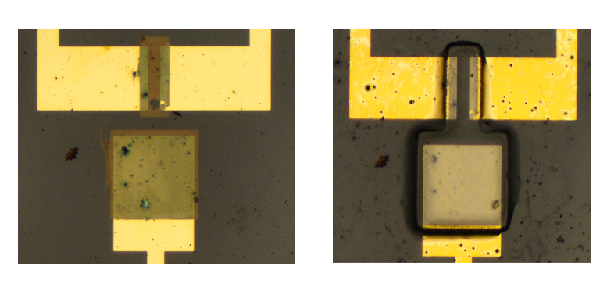
\includegraphics[width=6cm]{Images/pdf/und_photo.pdf} }}
    %\hspace{2em}
    \subfloat[]{{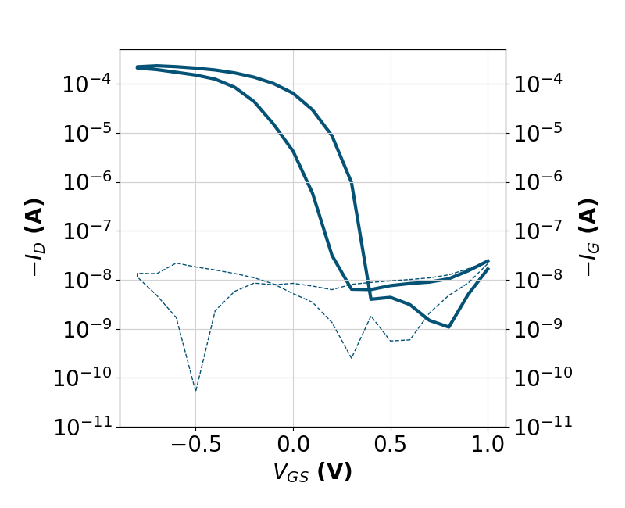
\includegraphics[width=7cm]{Images/pdf/transfer_photo_air.pdf} }}
    %\qquad
    %\subfloat[]{{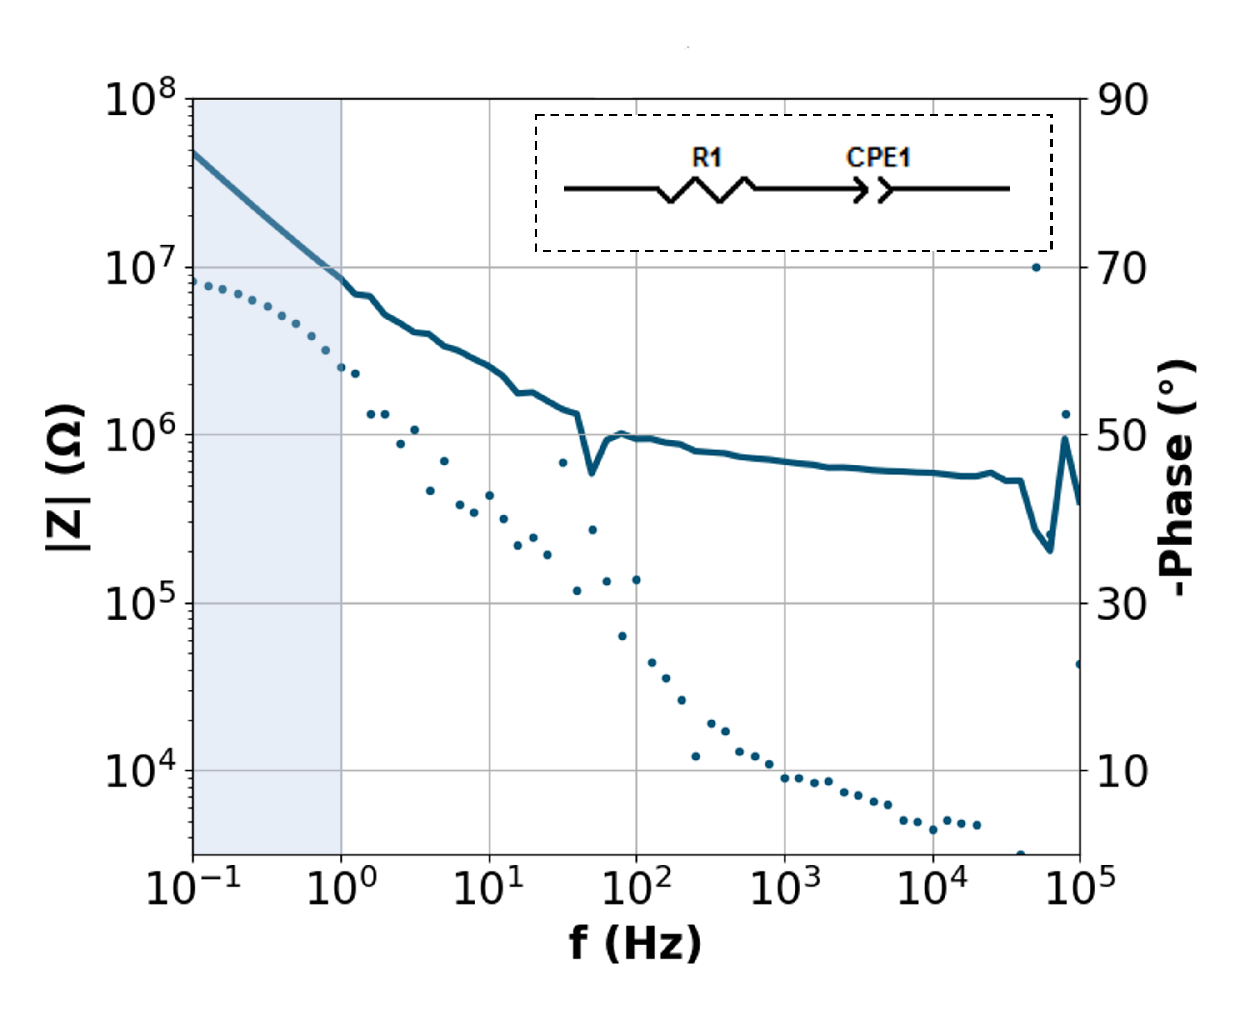
\includegraphics[width=6cm]{Images/pdf/EIS_photo.pdf} }}
    \subfloat[]{{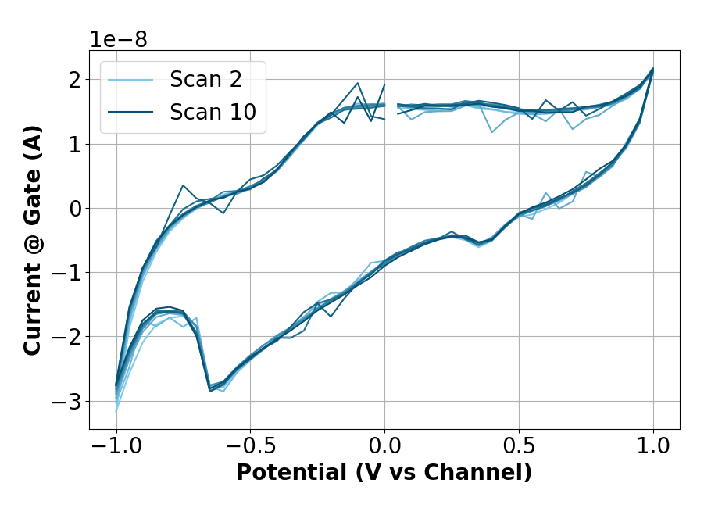
\includegraphics[width=7cm]{Images/pdf/CV_photo_air.pdf} }}
    \caption[Performance of solid-OECT with photolithographed SSE in ambient conditions]{a) Transfer characteristics at $V_{DS}$ of -0.1 V, and b) cyclic voltammograms, of same device from Figure \ref{fig:photoSSE}}
    \label{fig:photoSSEair}
\end{figure}

Calculated parameters of operational devices exposed to ambient conditions are shown in Table \ref{tab:photofom_amb}, an increase on transconductance compared to the N$_{2}$ environment condition is perceived, which aligns with the increase in current due to oxidation. The reported redox potentials represent the potential values close to the turn-on voltages, again they may not necessarily correspond to the most prominent peaks. Although the average redox values showed no hysteresis, differences were observed in most devices and in the transfer curves. 

Interestingly, devices exhibited prominent peak at -0.37 $\pm$ 0.08 V and -0.56 $\pm$ 0.09 V in the oxidation and reduction scans, respectively suggesting complex electrochemical processing occurring in our devices. While the oxidation of the polymer is evident, the occurrence of ORR and the generation of hydrogen peroxide cannot be ruled out during operation. These redox peaks could represent a more complex scenario where ORR is initiated either by the electrochemically doped p(g3T2-T) channel or by the biased p(g3T2-T) gate. Again, further controlled experiments are needed to confirm this hypothesis.

%% this needs the AgCl study instead

\begin{table}[ht]
\centering
\caption{Parameters extracted from the characterization of photopatterned SSE OECT under ambient conditions}
\begin{tabular}{l|c||l|c}
Parameters & Value & Parameters & Value \\\hline \hline
V$_{Th,forward}$ [V] & 0.36 $\pm$ 0.05 & V$_{Th,backward}$ [V] & 0.25 $\pm$ 0.13 \\
& & &\\[-1em]
%C$_{channel}$ [nF] &  & C* [Fcm$^{-3}$] &  \\
%& & &\\[-1em]
V$_{ox}$ [V] & 0.40 $\pm$ 0.11 & V$_{red}$ [V] & 0.40 $\pm$ 0.09 \\
& & &\\[-1em]
|g$_{m,max}$| [$\mu$S] & 315 $\pm$ 44 &  &\\\hline
\end{tabular}
\label{tab:photofom_amb}
\end{table}

%\newpage
\subsection{Undoped Inkjet-Printed SSE}%Solid-State Electrolyte}
%The Ag/AgCl gate electrode’s work function is reasonably constant, the work function of an OMIEC gate electrode however may vary depending on its processing history and redox reactions with other species present in the electrolyte (e.g. molecular oxygen).28 Applying VGS only determines the potential difference between the gate and channel but does not control the potentials of either electrode (hence the position of the Fermi level) with respect to a reference. This leads to many challenges in operating an OECT with OMIEC gate electrodes \cite{tanOperationMechanismOrganic2021}.

While photopatterned SSE offered an approach to obtain microstructuring devices with high yields and relatively good performances, the removal of non-crosslinked SSE is not as efficient, the method potentially leaves residual material that can lead to device crosstalk and leakage. Ink-jet printing represents a promising approach to address this limitation \cite{tsengThresholdVoltageControl2023}. However, to ensure good printing, the adhesion promoter step remains crucial and, as commented before, aids in reversing the oxidation of p(g3T2-T).

For this trial, patterning process yielded a total of seven devices. However, issues with film uniformity resulted in only four devices being successfully printed. This may have been caused by contamination or improper coating of the adhesion promoter. Among these four devices, only one was fully operational, and it will be used in the subsequent analysis.

The printing process takes approximately two hours per sample under ambient conditions. Efforts were made to set the printing parameters using a different sample while subjecting our device to high temperatures and ethanol rinsing. Unfortunately, the resulting device still exhibited signs of oxidation, as will be shown in the analysis.

Figure \ref{fig:printedSSE} illustrates all the mentioned measurements, and Table \ref{tab:printedfom} presents the calculated parameters. Threshold voltages calculated between scans show minimal difference, indicating almost no hysteresis, so only one value is reported. Importantly, V$_{Th}$ is no longer negative; there is a shift towards positive values (oxidation), resulting in a higher transconductance.

%printed i only have one, U5
\begin{figure}[ht]
    \centering
    \subfloat[]{{\includegraphics[width=7cm]{Images/pdf/und_ink.pdf} }}
    \subfloat[]{{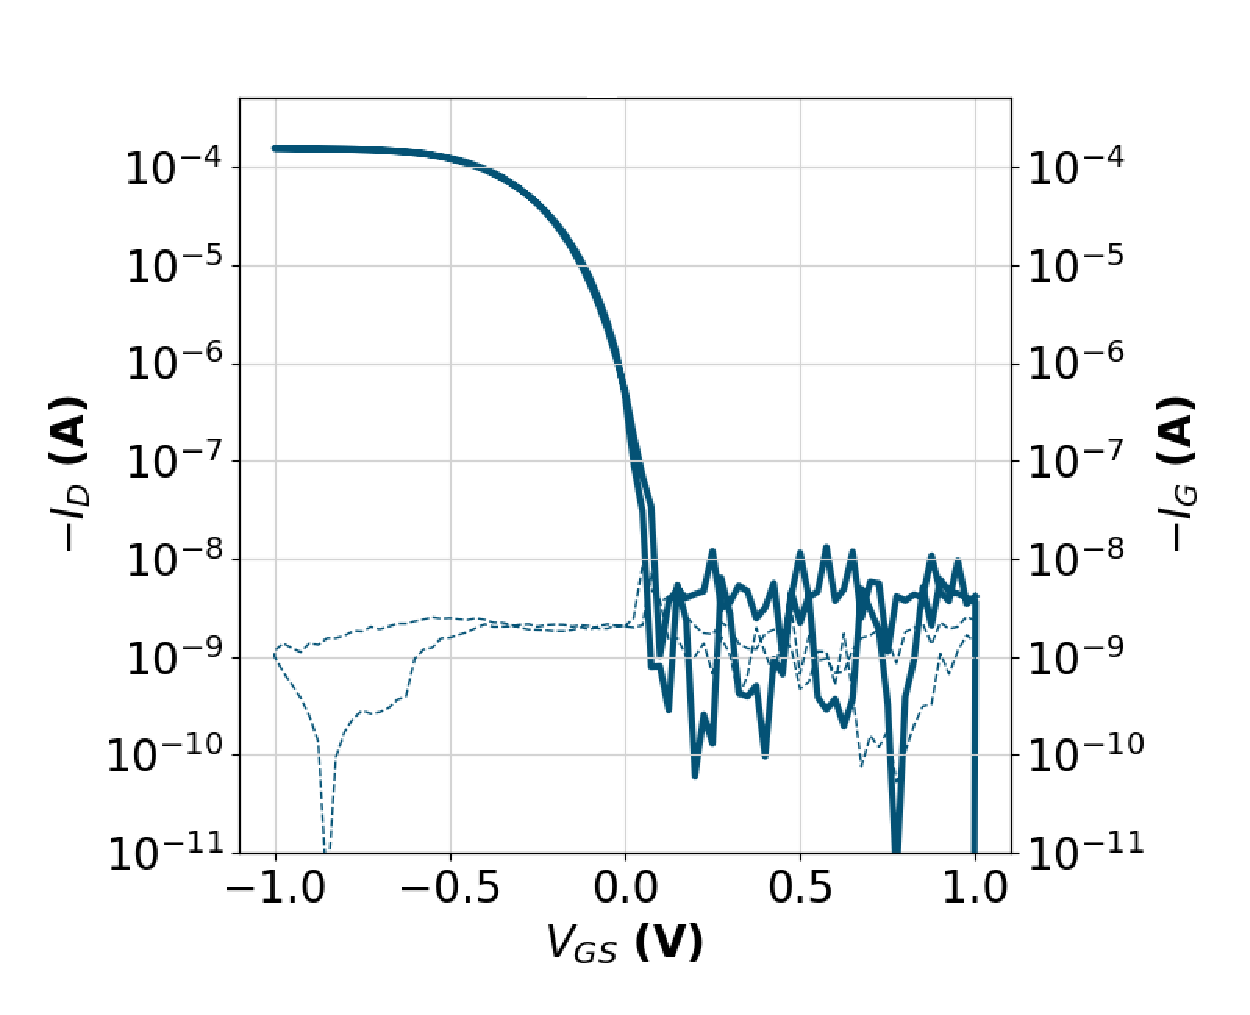
\includegraphics[width=7cm]{Images/pdf/transfer_ink.pdf} }}
    \qquad
    \subfloat[]{{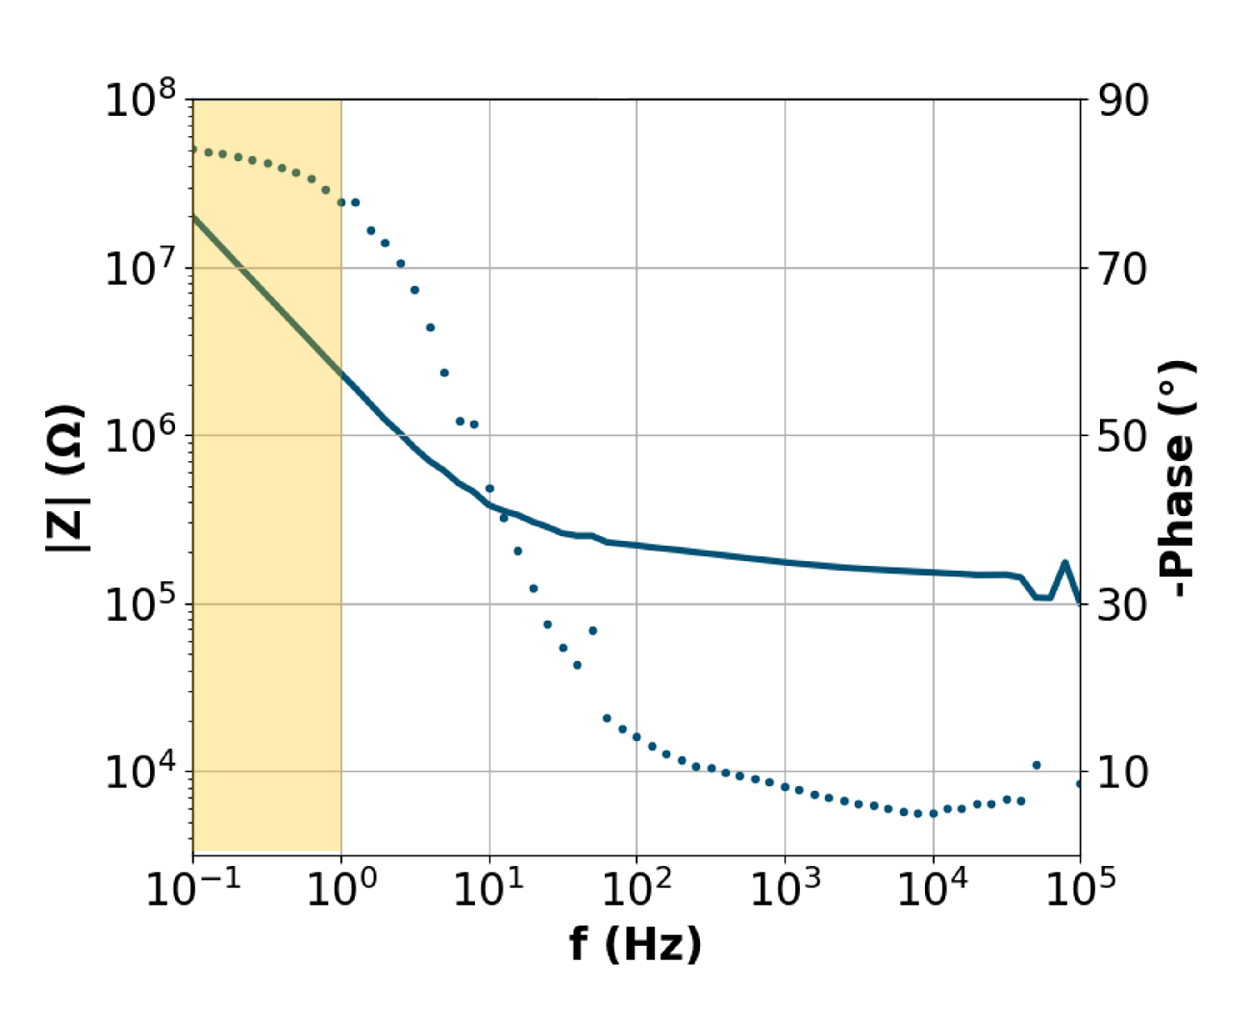
\includegraphics[width=7cm]{Images/pdf/EIS_ink.pdf} }}
    \subfloat[]{{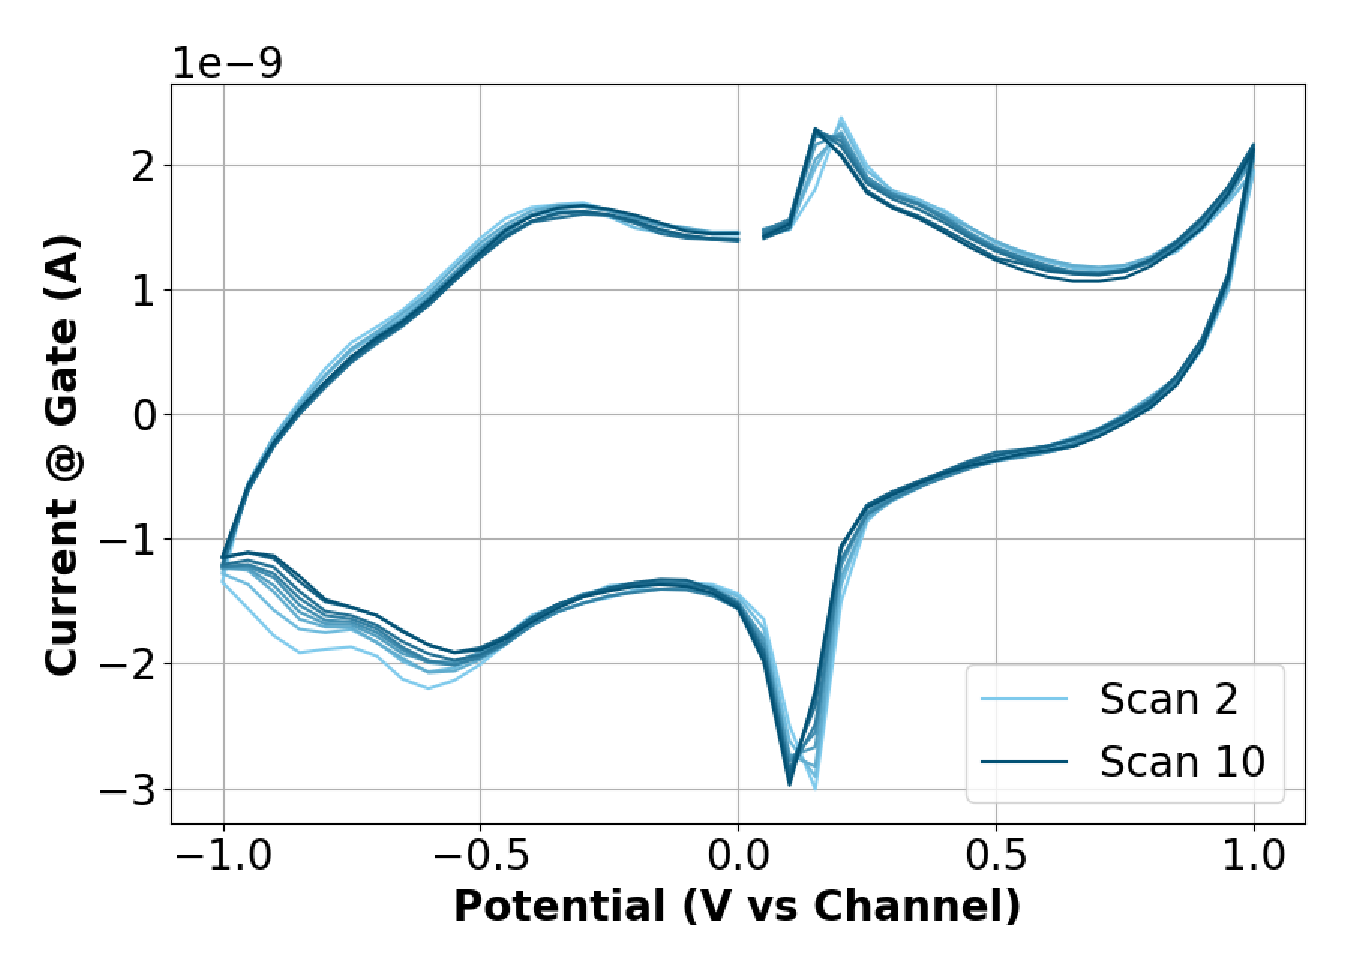
\includegraphics[width=7cm]{Images/pdf/CV_ink.pdf} }}
    \caption[Performance of solid-OECT with printed SSE]{a) Micrograph of patterned device with printed SSE, b) transfer characteristics at $V_{DS}$ of -0.1 V. c) Bode plot obtained by EIS and d) cyclic voltammograms.}
    \label{fig:printedSSE}
\end{figure}

The channel capacitance and volumetric capacitance also exhibit an increase in value, which is reflected in higher $I_{ON}$. Furthermore, cyclic voltammograms show predominant peaks close to the turn-on voltages but also secondary peaks in the oxidation scan at -0.33 V and +1.0 V, and in the reduction scan at -0.55 V. 

\begin{table}[ht]
\centering
\caption{Parameters extracted from the characterization of printed SSE OECT}
\begin{tabular}{l|c||l|c}
Parameters & Value & Parameters & Value \\\hline \hline
V$_{Th}$ [V] &  0.13 & |g$_{m,max}$| [$\mu$S] & 355 \\
& & &\\[-1em]
C$_{channel}$ [nF] & 85.3 & C* [Fcm$^{-3}$] & 91.6 \\
& & &\\[-1em]
V$_{ox}$ [V] & 0.15 & V$_{red}$ [V] & 0.09 \\\hline
\hline
\end{tabular}
\label{tab:printedfom}
\end{table}

In conclusion, it appears that the undoped p(g3T2-T) sample is not compatible with the printed SSE process. Its extended exposure time to environmental conditions, leading to unavoidable oxidation, prevents the attainment of an accumulate-mode OECT. New methods to counteract this oxidation are needed if printed SSE is to be used, or photolithography should be considered, despite the possible device crosstalk.

%\newpage
\subsection{Doped Inkjet-Printed SSE} \label{subsec:dopedOECTs}
%\subsection{Doped-p(g3T2-T) with Threshold Voltage Shift} \label{subsec:dopedOECTs}
Doped p(g3T2-T) has been demonstrated to be stable under ambient conditions, and owing to the advantages of printed SSE, this method will be the chosen approach for SSE application in this subsection. 

Different doping levels were intended to be studied in this subsection. However, only 5 mg/mL of F$_{6}$TCNNQ resulted in doping homogeneity suitable for meaningful comparison with undoped p(g3T2-T). Figure \ref{fig:unhom} reveals irregularities in doping when using a new vial of 10 mg/mL dopant concentration, and the same issue was observed for vials prepared with 15 mg/mL dopant. Acetonitrile was unable to correctly dissolve this dopant at high concentrations, which was not observed with F$_{4}$TCNQ and one initial vial of 10 mg/mL F$_{6}$TCNNQ. Consequently, achieving depletion-mode OECTs with higher and homogeneous doping levels was not possible.

\begin{figure}[ht]
    \centering
    \includegraphics[width=10cm]{Images/pdf/unhom_doping.pdf} 
    \caption[Inhomogeneous doping issues]{Micrograph of inhomogeneous doping in sample.}
    \label{fig:unhom}
\end{figure}

%\subsubsection{Channel conductivity}
From the experiments conducted with undoped p(g3T2-T) in Subsection \ref{subsec:revox}, it was observed that upon UV light exposure, the electrochemical de-doping of a device was no longer irreversible. Therefore, as a first step, the channel conductivity was monitored with SSE on top. The sample with 5 mg/mL dopant maintained a conductivity of 4 $\mu$S for two hours with some fluctuation and approximately 10\% drop in conductivity. While some conductivity was lost, it was not a significant drop of orders of magnitude. 

%\subsubsection{Solid-OECT performance}
The adhesion promoter used for undoped p(g3T2-T) could not be used for doped species since it will remove dopants during the application steps. An alkaline adhesion promoter would be needed, which required additional experiments to test its effectiveness and correct application. Therefore, no promoter was used at this stage, so low yields in printing were expected, despite the high yields in patterning.

Eight operational devices were obtained. However, only one exhibited a capacitive behavior that allowed for the measurement of transfer characteristics, and it will be used in this analysis. %The low yield may be due to remaining material shorcircuiting channel (etching step was not enough).
Transfer characteristics, EIS, and CV measurements are shown in Figure \ref{fig:dopedSSE}, and the calculated parameters are exhibited in Table \ref{tab:dopedfom}.

%% U7
\begin{figure}[ht]
    \centering
    \subfloat[]{{\includegraphics[width=3.5cm]{Images/pdf/doped_ink.pdf} }}
    \subfloat[]{{\includegraphics[width=7cm]{Images/pdf/transfer_doped.pdf} }}
    \qquad
    \subfloat[]{{\includegraphics[width=7cm]{Images/pdf/EIS_doped.pdf} }}
    \subfloat[]{{\includegraphics[width=7cm]{Images/pdf/CV_doped.pdf} }}
    \caption[Performance of solid-OECT with doped-p(g3T2-T)]{a) Micrograph of patterned device with printed SSE, b) transfer characteristics at $V_{DS}$ of -0.1 V. c) Bode plot obtained by EIS and d) cyclic voltammograms.}
    \label{fig:dopedSSE}
\end{figure}

Despite the use of doped p(g3T2-T), the threshold voltage remains slightly negative. A positive shift has been achieved when compared with undoped p(g3T2-T) with the lowest conductivity. However, the shift achieved by oxidized p(g3T2-T) is significantly higher. 

It is important to note that it is not certain that this value corresponds to the mentioned doping level. This uncertainty arises because under ambient conditions, doped p(g3T2-T) upon contact with SSE precursor, experiences a significant drop in conductivity within the first 15 minutes at $V_{DS}$ of -0.1 V, as discussed in Subsection \ref{subsec:stab}. Therefore, during the time between the printing process and the crosslinking of SSE, it is possible that this effect took place in our device, albeit at a lower rate since it was not biased. Further experiments are needed to confirm this hypothesis.

A noisy EIS spectrum was obtained, possibly due to environmental factor or a defect in the gate electrode that is perceived in the micrograph. Calculations of the channel and volumetric capacitance was made using the dotted line, where an expected tred was identified. High channel capacitance and volumetric capacitance were calculated, as expected, but new devices are needed to confirm this value.  %*needs to be measure again*

Additionally, cyclic voltammograms show predominant peaks close to turn-on voltages but also secondary peaks in the oxidation scan at -0.25 and +1.0 V, and in the reduction scan at -0.33 V. 

\begin{table}[ht]
\centering
\caption{Parameters extracted from the characterization of doped-p(g3T2-T) OECT}
\begin{tabular}{l|c||l|c}
Parameters & Value & Parameters & Value \\\hline \hline
V$_{Th}$ [V] & -0.10 & |g$_{m,max}$| [$\mu$S] & 567 \\
C$_{channel}$ [nF] & 130 & C* [Fcm$^{-3}$] &  140 \\
%C$_{channel}$ D6 [nF] & 289 & C* [Fcm$^{-3}$] & 311 \\
V$_{ox}$ [V] & 0.10 & V$_{red}$ [V] & 0.0 \\\hline
\end{tabular}
\label{tab:dopedfom}
\end{table}

%Achieving effective charge transfer between the analyte and OMIEC requires appropriate alignment of the electrochemical potential of electrons on the OMIEC electrode and the redox specie. Failure to do so may result in the subsequent transfer of charges to other redox-active sinks in the environment, leading to undesirable side reactions and products that may interfere with the OMIEC’s operation. Electrons flow from a region of higher to lower electrochemical potential. Hence, achieving electron transfer from redox-active species to the OMIEC requires the latter to have a deep LUMO (high electron affinity) \cite{tanMixedIonicElectronic2022} %paper

%\newpage
\subsection{Threshold Voltage Shift in OECTs} \label{subsec:vth_shift}

Having performed individual analysis of each fabricated device, including important OECT figures of merit such as transconductance, volumetric capacitance and redox potentials, %the latter mainly to our approach of using doped p(g3T2-T) gates. In this subsection, 
our focus in this subsection is now on the threshold voltage and, more importantly, the expected shift upon doping.

Figure \ref{fig:vth_shift_final} exhibits the threshold voltage of all operating devices for each sample described in this section.

\begin{figure}[ht]
    \centering
    \includegraphics[width=\textwidth]{Images/pdf/Vth_shift_plot.pdf} 
    \caption[Threshold voltage shift of all studied devices]{Threshold voltage of all studies samples including error bars from operating device in each group.}
    \label{fig:vth_shift_final}
\end{figure}

It was found that electrochemical de-doping of p(g3T2-T) prior exposure to UV light of the SSE precursor produced the most negative threshold voltages, although with high variability. This may be attributed to various factors, such as devices not being directly impacted by the electrochemical de-doping (only one device is de-doped and not included in this calculation), resulting in different degrees of de-doping, or defect within the photolithography process. 

More importantly, the device fabricated using p(g3T2-T) doped with 5 mg/mL F$_{6}$TCNNQ dopant concentration exhibits a threshold voltage that is slightly shifted towards positive values, the unwanted oxidation of p(g3T2-T) with molecular oxygen achieves positive values more effectively, allowing the fabrication of accumulation-mode OECTs. The cause of the low threshold voltage shift was previously discussed, and it is likely due to the extended time between printing and exposure, during which TCNNQ$^{-}$ anions may be drawn away to the SSE or compensation doping occurs upon contact with SSE precursor during the printing process. In either case, further studies are necessary to determine which hypothesis is more accurate in order to counteract this effect. For the former, an adhesion promoter before the application of dopants may be a possible solution. Additionally, applying photopatterned SSE may yield better results, as the effect will still occur but time between application and exposure is much shorter.



 

%\section{Conclusion}
%\lipsum[86-88]

%%% Local Variables: 
%%% mode: latex
%%% TeX-master: "thesis"
%%% End: 
